\chapter{LIMBERO-GRIEEL, Hardware and Software}
\label{ch:chapter_four}%

In this chapter, LIMBERO-GRIEEL, the robotic system used for this research is presented. Defining its configuration is important to understand its purpose and the problems addressed in the next chapters. 

\textbf{LIMBERO} (\textbf{LIMB}-climbing \textbf{E}xploration \textbf{RO}bot) is a prototype omnidirectional four-limbed robot, designed, 3D printed, and assembled by the Limb Team at the Space Robotics Lab \cite{SRL}(SRL) (led by Professor Yoshida Kazuya at Tohoku University, Japan). It is a small lightweight climbing robot, with a claw-type gripper\cite{passiveSpineTohoku} in its default design.\\
\textbf{GRIEEL} (\textbf{GRI}pper wh\textbf{EEL}) is a prototype gripper-wheel transformable mechanism, designed and patented by Masahiro Uda \textit{est all}\cite{GrieelUda}\cite{GRIEELUdaThesis}, member of the SRL Rover Team.  

\textbf{LIMEBRO-GRIEEL} is obtained from the assembly of the two systems described above, enabling wheeled locomotion in addition to walking and climbing. 
The overall system used in this research is still in the early stages of development, and a new version of GRIEEL (here referred to as GRIEELv2) has been already developed, as new limbs for LIMBERO-GRIEELv2. 
Chapter \ref{ch:chapter_nine} presents briefly these new versions of the prototypes. 

The robotic structure used during this research is described in terms of its hardware structure and the ROS2 control software architecture. Then, the Gazebo and MATLAB-Simulink simulation is briefly described, the first used to validate the motion control software and the additional algorithm implemented (described in chapter \ref{ch:chapter_five}), the second to tune the joints controllers and analyze the base manipulability ellipsoid, described in the previous chapter. 

\newpage 

\section{Hardware Description}
\label{sec:hardware}

The Hardware is described in this section, first with an overview of the limb structure and its actuated joints, and an explanation of how the gripper-wheel mechanism works and what are the two main mode configurations. Finally, the servo motors used to control the joints are listed.   

\subsection{Limb Description}
\label{sec:limb}
In its current design, LIMBERO is an omnidirectional quadruped with $4-DOF$ insect leg topology (different legs' views are represented in Fig.\ref{fig:LIMBERO_limb}) \cite{Todd}\cite{LeggedRObotBiomechanics}\cite{ReviewLegged}, in particular the choice of this structure comes from the studies of Kentaro Uno on HubRobo \cite{HubRobo}. 
In his PhD dissertation \cite{KentaroUnoPhD}, he proved that for climbing locomotion, the insect configuration results in
being more stable, energy-efficient, and versatile at once.


GRIEEL is the transformable end effector module (represented in Fig.\ref{fig:Gripper_Wheel}), but here this name is used to refer to the overall actuated mechanism, composed of the module and a $3-DOF$ mounting mechanism used for limb attachment, configuration change, and driving locomotion \cite{GRIEELUdaThesis} (represented in Fig.\ref{fig:GRIEEL_GRIPPER_WHEEL}).   


\begin{figure}[H]
    \centering
    \subfloat[\label{fig:Limbero_sideVIEW2}]{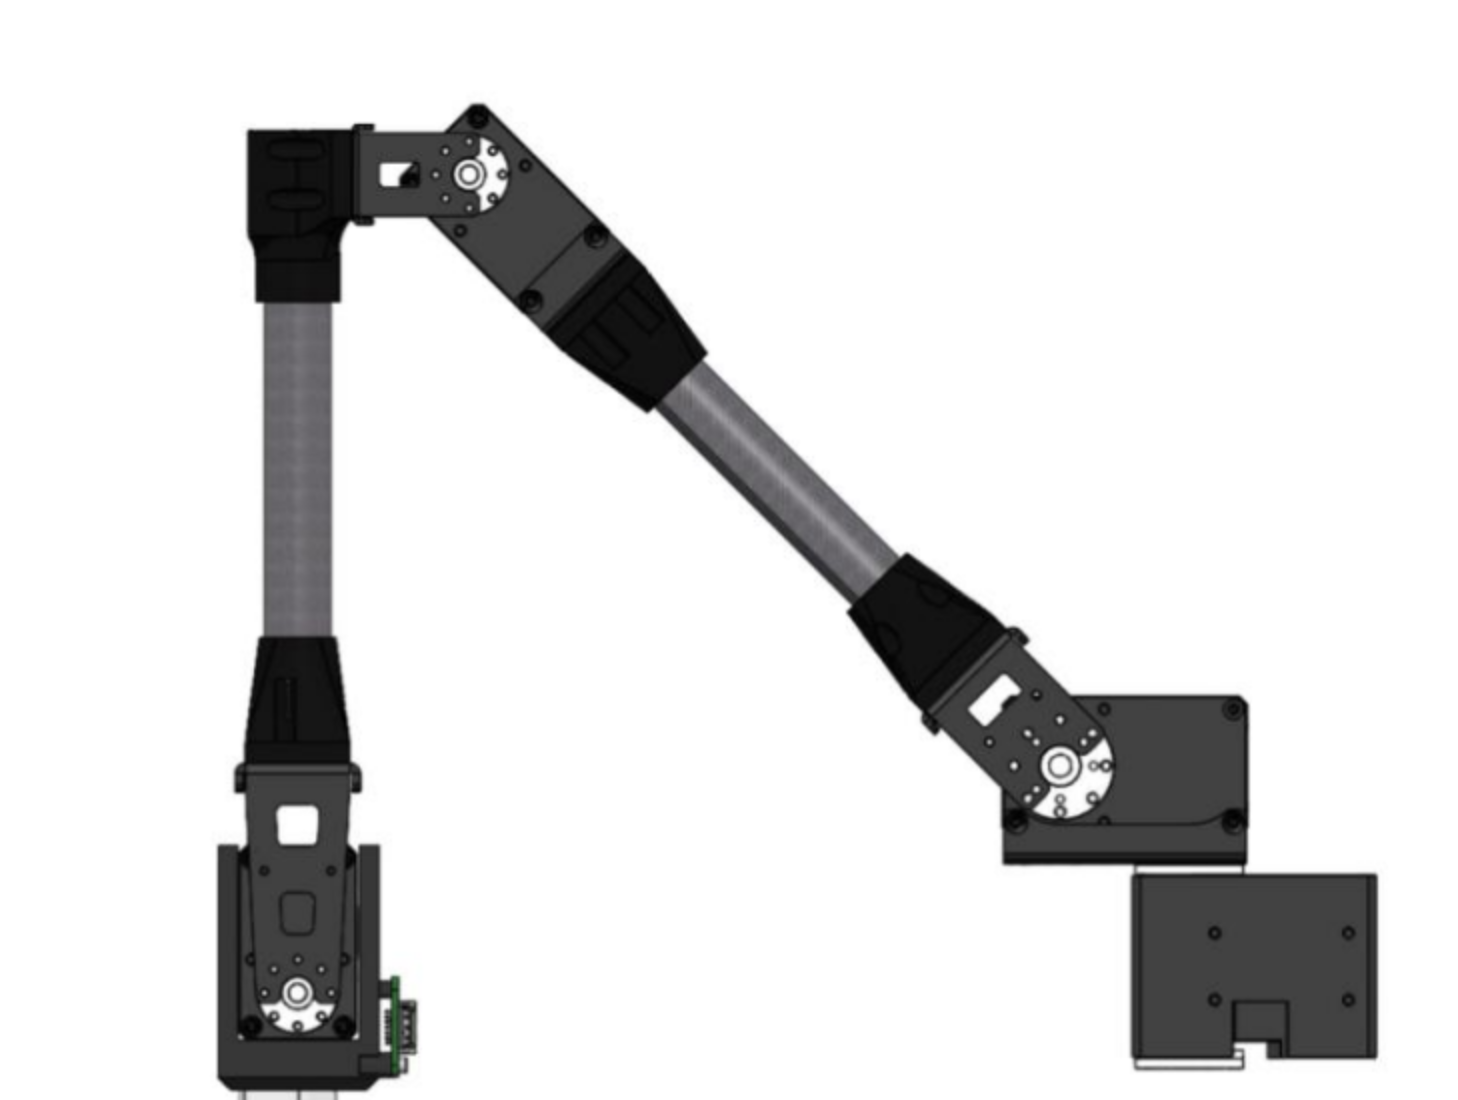
\includegraphics[scale=0.1]{Images/img_ch4/limbero_sideVIEW2.png}}
    \subfloat[\label{fig:Limbero_orthoVIEW}]{\includegraphics[scale=0.1]{Images/img_ch4/Limbero_orthoVIEW.png}}\\
    \subfloat[\label{fig:Limbero_sideVIEW1}]{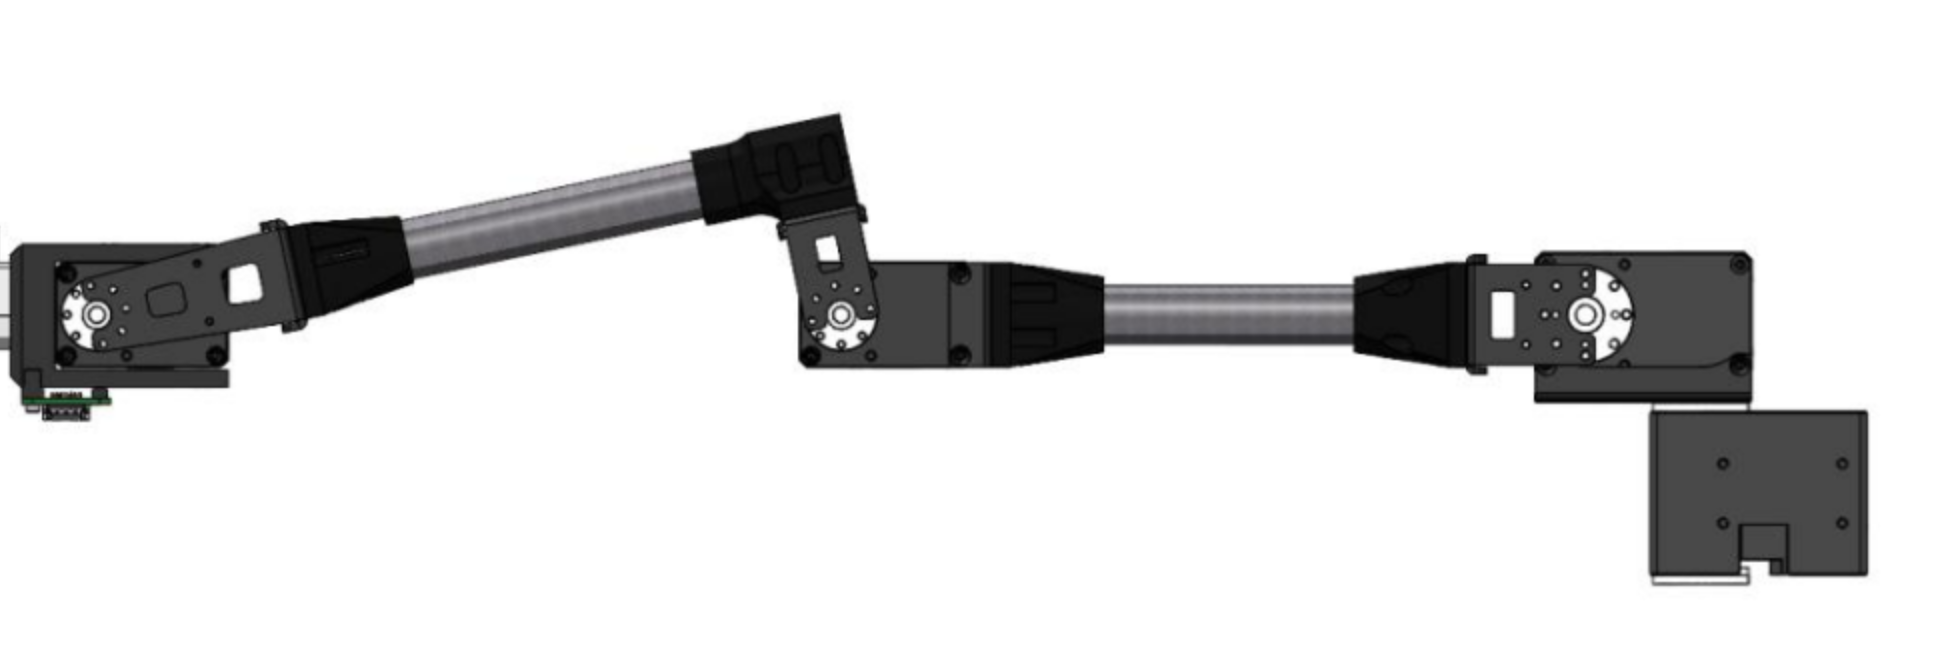
\includegraphics[scale=0.1]{Images/img_ch4/limbero_sideVIEW1.png}}
    \caption[Different views of LIMERO limb model]{\cite{LIMBEROTakadaThesis} Views of LIMERO limb model, without the claw-type gripper EE, (a) and (b) are in the same configuration, while (c) is in the zero joints configuration}
    \label{fig:LIMBERO_limb}
\end{figure}

\begin{figure}[H]
    \centering
    \subfloat[Gripper-Wheel module.\label{fig:Gripper_Wheel}]{\includegraphics[scale=0.20]{Images/img_ch4/Gripper_Wheel.png}}
    \\
    \subfloat[actuated GRIEEL mechanism in the two modes.\label{fig:GRIEEL_GRIPPER_WHEEL}]{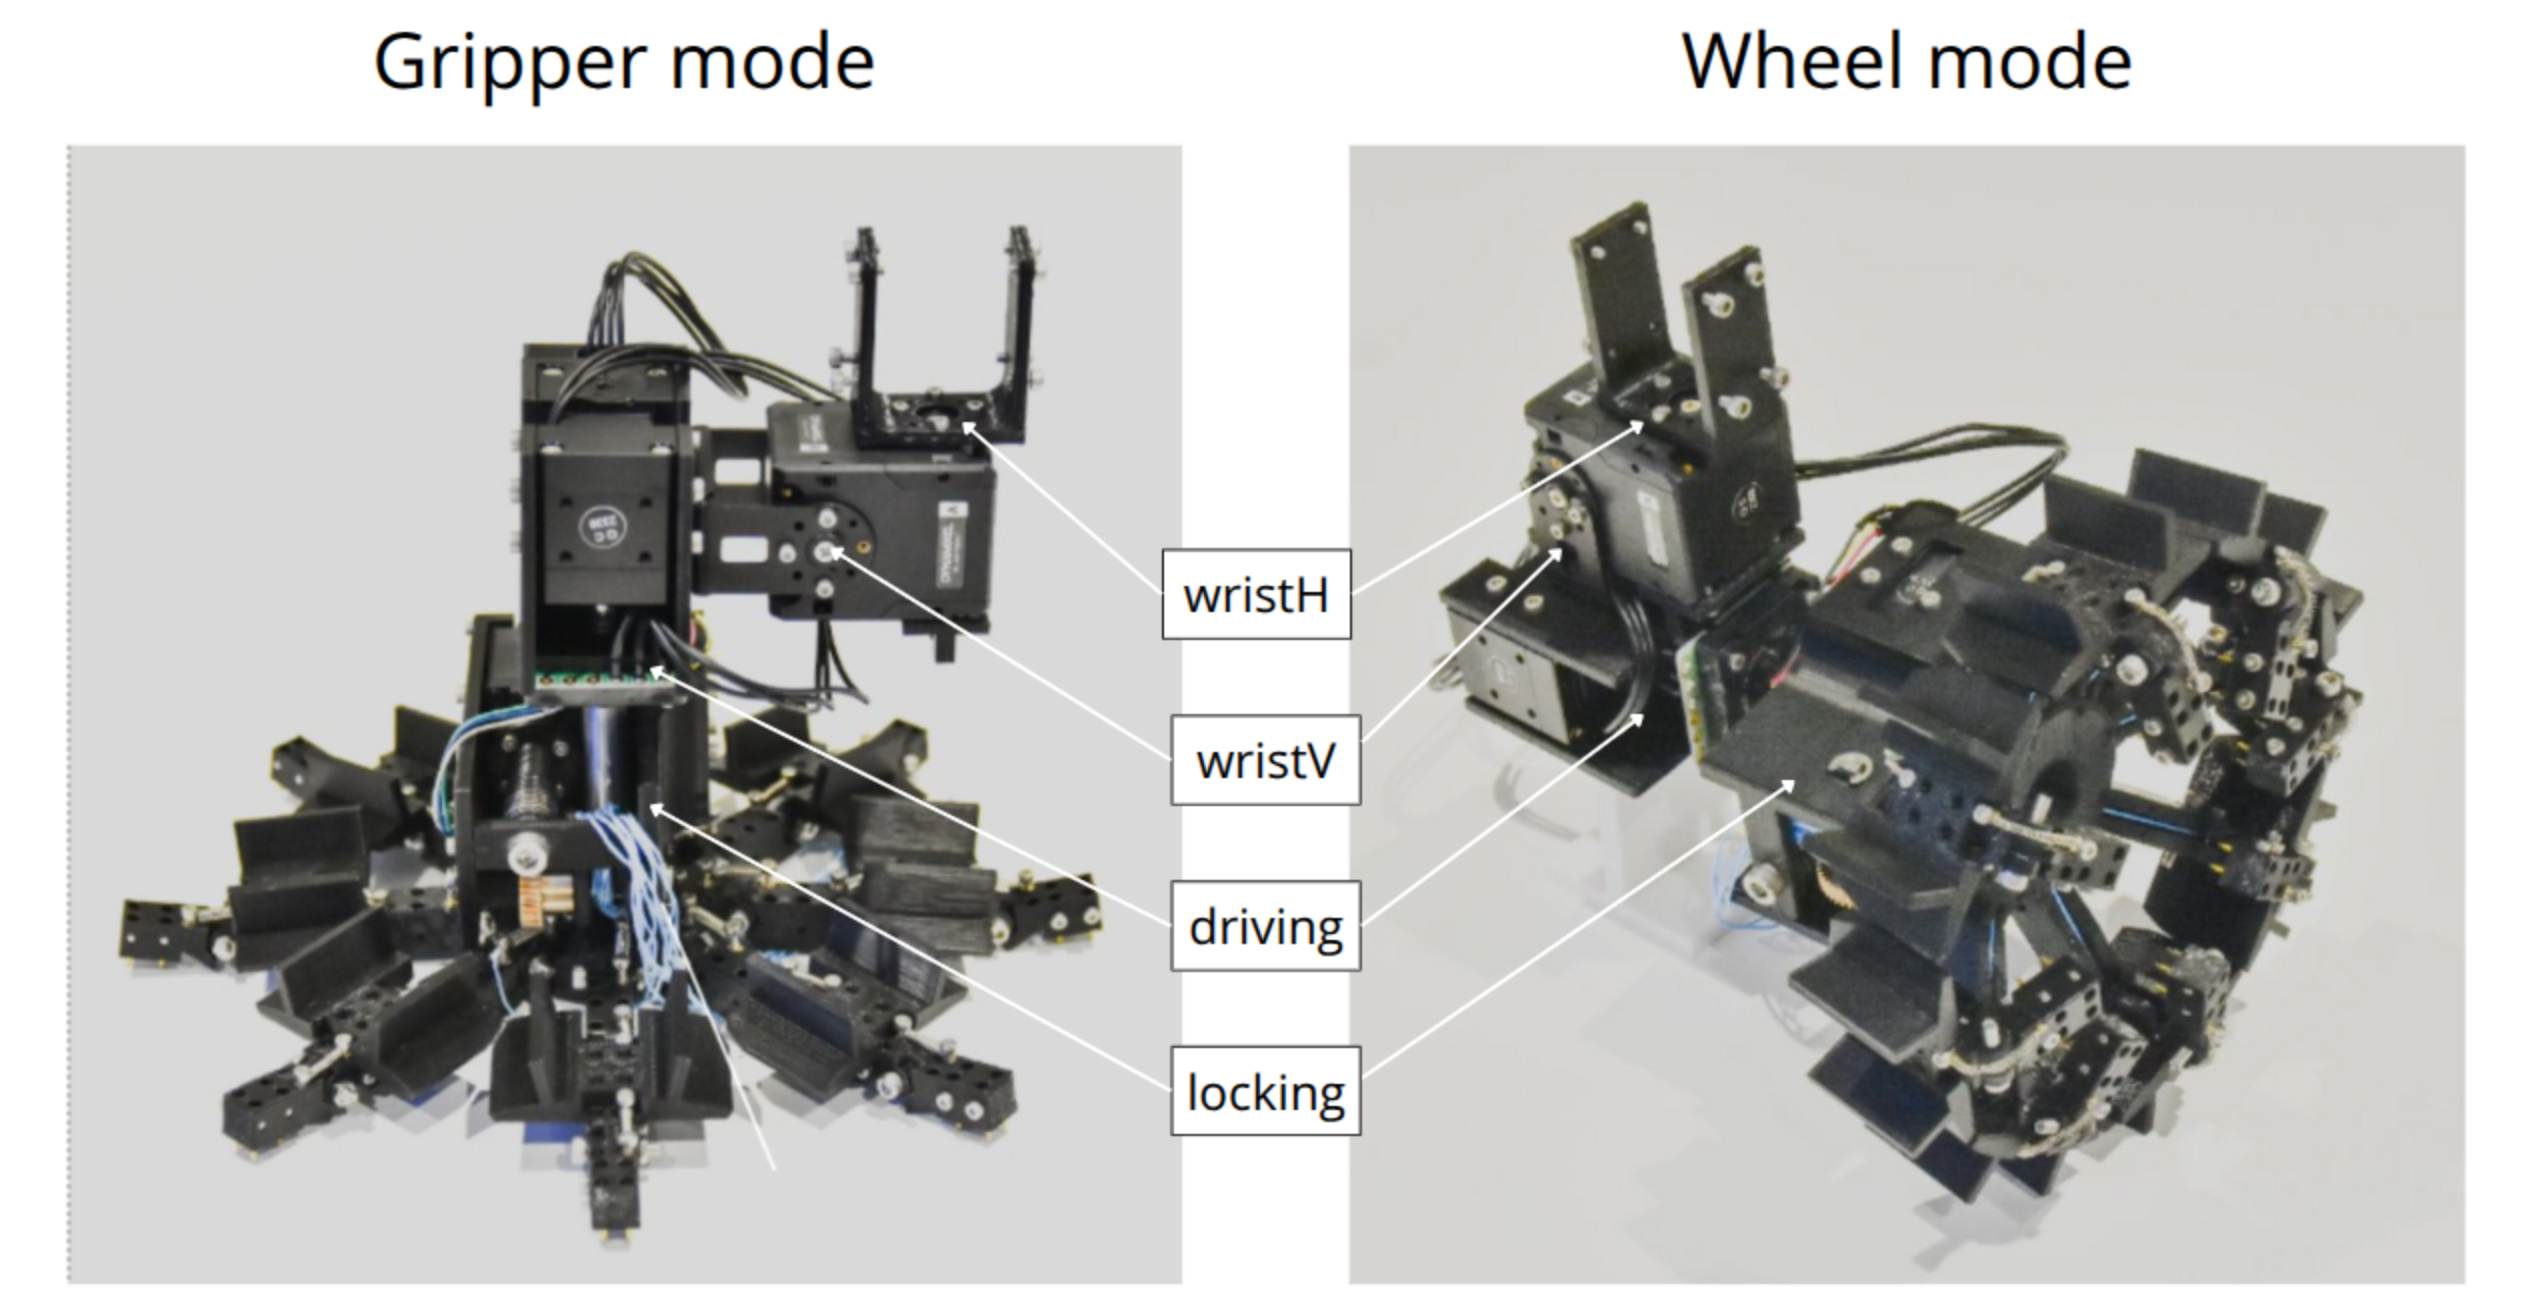
\includegraphics[scale=0.15]{Images/img_ch4/GRIEEL_GRIPPER_WHEEL.png}}
    \caption[GRIEEL module and actuation mechanism]{GRIEEL module and actuation mechanism}
    \label{fig:GRIEELMechanism}
\end{figure}

The assembled limb structure, with its $7-DOF$ is a redundant system on the 6-dimensional position and orientation task space of its limb tip  (the model and the real limb are represented in Fig.\ref{fig:LIMBERO_GRIEEL_limb}, and the equivalent schematic model in Fig.\ref{fig:LIMBERO_GRIEEL_limb_model}). 
Introducing some names, with the notation introduced in chapter \ref{sec:kinematic}, the set of limbs here defined as $J = \{LF, LH, RH, RF \}$ (Left Front, Left Hind, Right Hind and Right Front), and the joint space of each limb $\mathbf{q}_j \in \mathbb{R}^7, \forall j\in J $, where the joints have the following names:\\
$q_{j,i} \in \{ j\_B2C, j\_C2F,  j\_F2T, j\_T2E,j\_wristH, j\_wristV, j\_driving\}$, as ordered in the serial kinematic structure. The names of the joints come from a common naming convention for the limb links in walking robots, for LIMBERO ordered as {limb\_root, coxa, femur, tibia, limb\_end}  and with a wrist notation for GRIEEL {wristH(orizontal), wristV(ertical), driving, gripper/wheel}.
The overall structure of the links' interconnection is represented in Fig.\ref{fig:TFTree_NOFINGERS} below.  
 
\begin{figure}[H]
    \centering
    \subfloat[Side view in gripper mode.\label{fig:LIMBERO_GRIEEL_GRIPPER_side}]{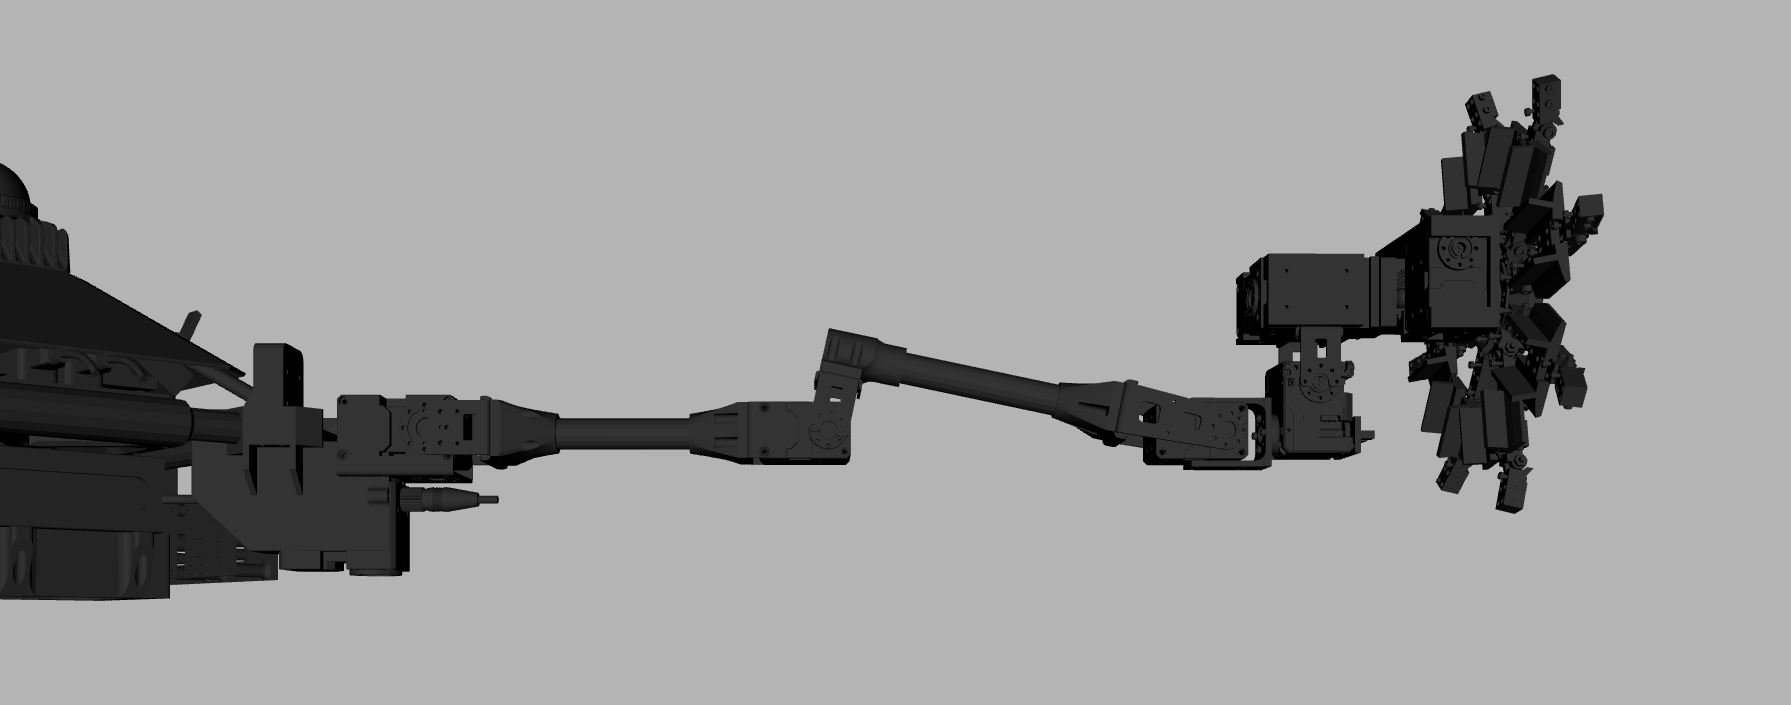
\includegraphics[width=0.4\textwidth]{Images/img_ch4/LIMBERO_GRIEEL_GRIPPER_side.png}}  \quad \subfloat[Side view in wheel mode.\label{fig:LIMBERO_GRIEEL_WHEEL_side}]{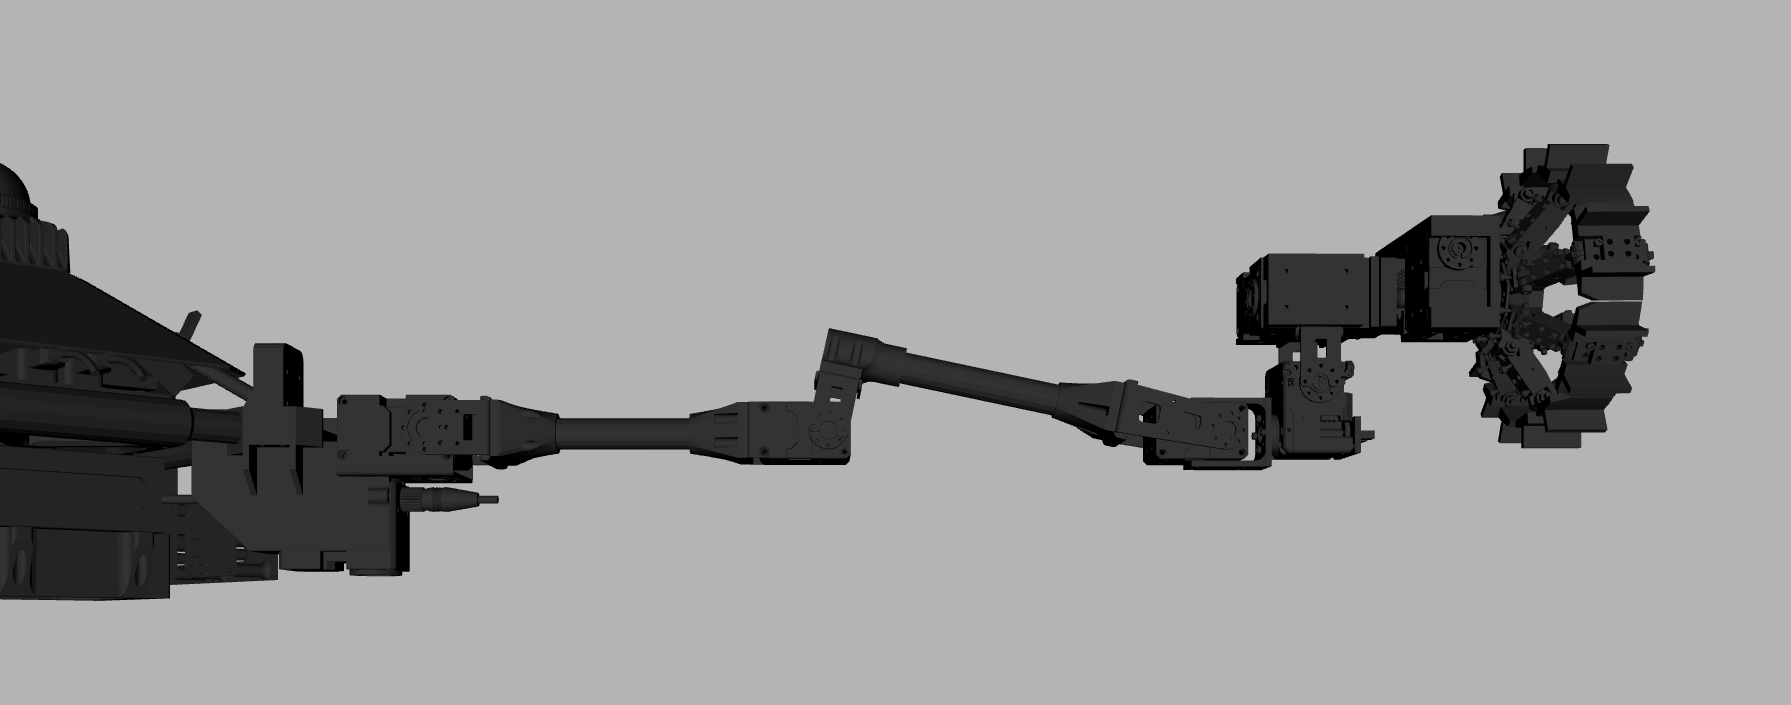
\includegraphics[width=0.4\textwidth]{Images/img_ch4/LIMBERO_GRIEEL_WHEEL_side.png}}
    \\
    \subfloat[Top view in gripper mode.\label{fig:LIMBERO_GRIEEL_GRIPPER_top}]{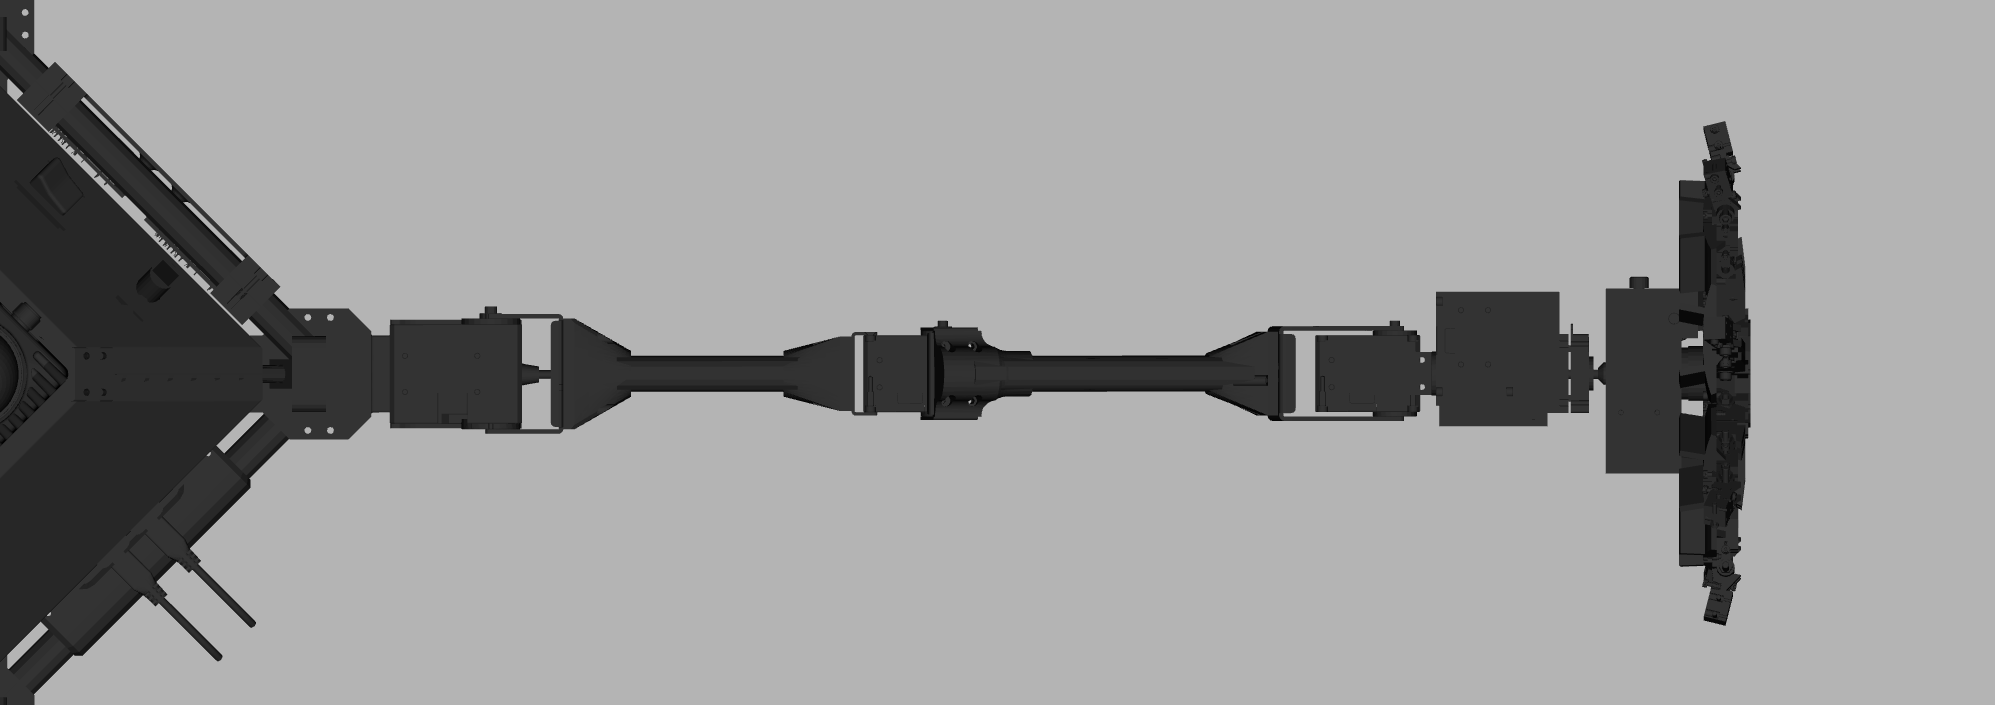
\includegraphics[width=0.4\textwidth]{Images/img_ch4/LIMBERO_GRIEEL_GRIPPER_top.png}}   \quad
    \subfloat[Top view in wheel mode.\label{fig:LIMBERO_GRIEEL_WHEEL_top}]{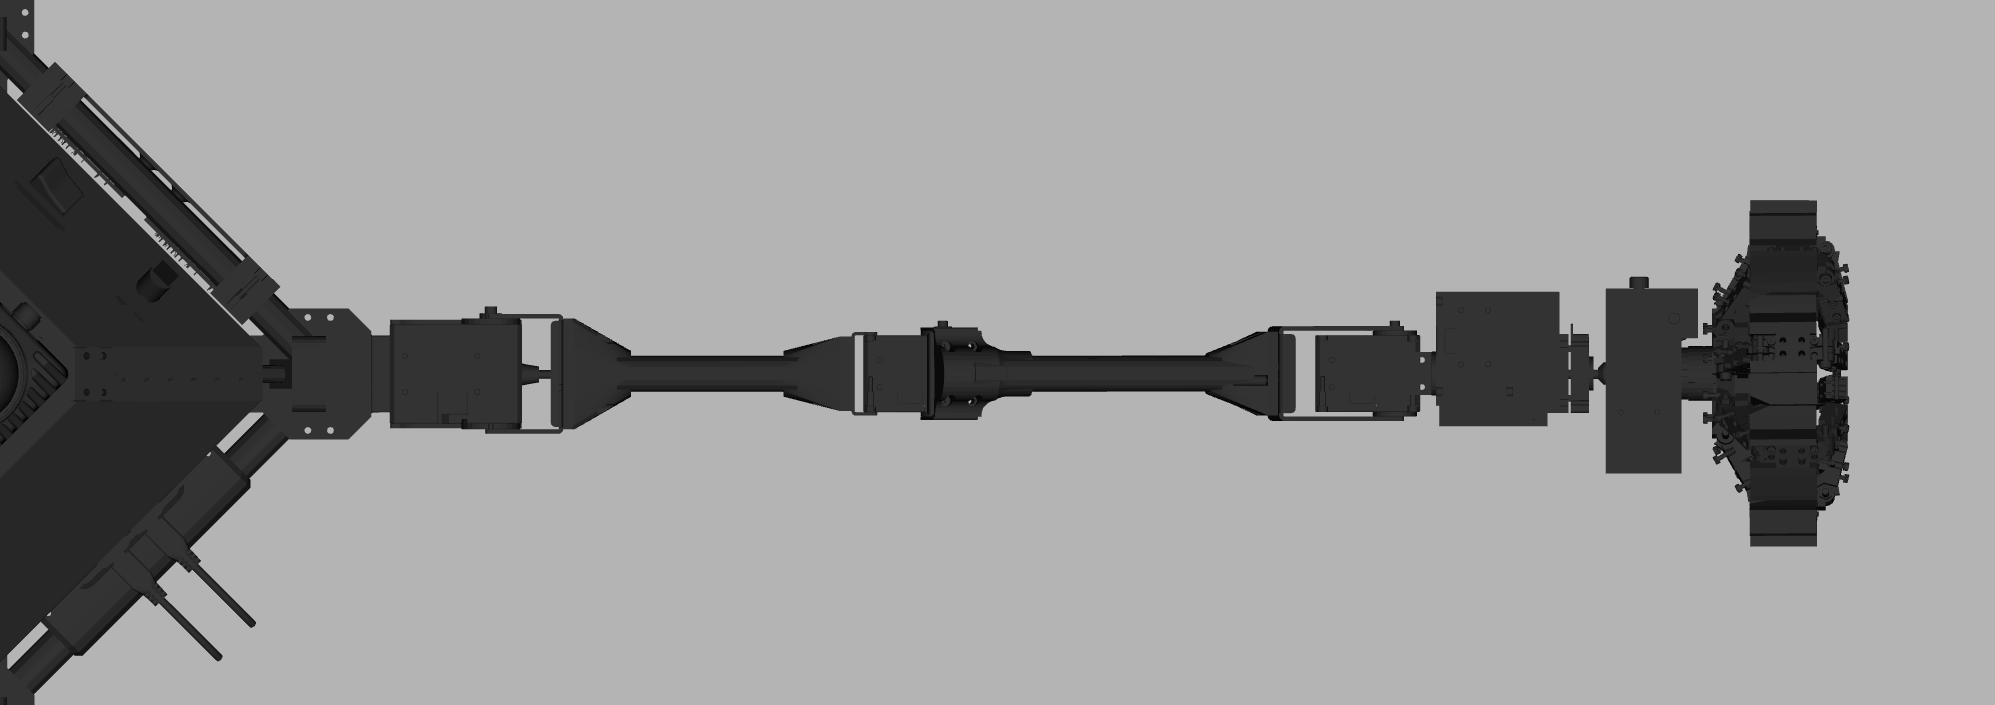
\includegraphics[width=0.4\textwidth]{Images/img_ch4/LIMBERO_GRIEEL_WHEEL_top.png}}
    \\
    \subfloat[Perspective view in gripper mode.\label{fig:LIMBERO_GRIEEL_GRIPPER_ortho}]{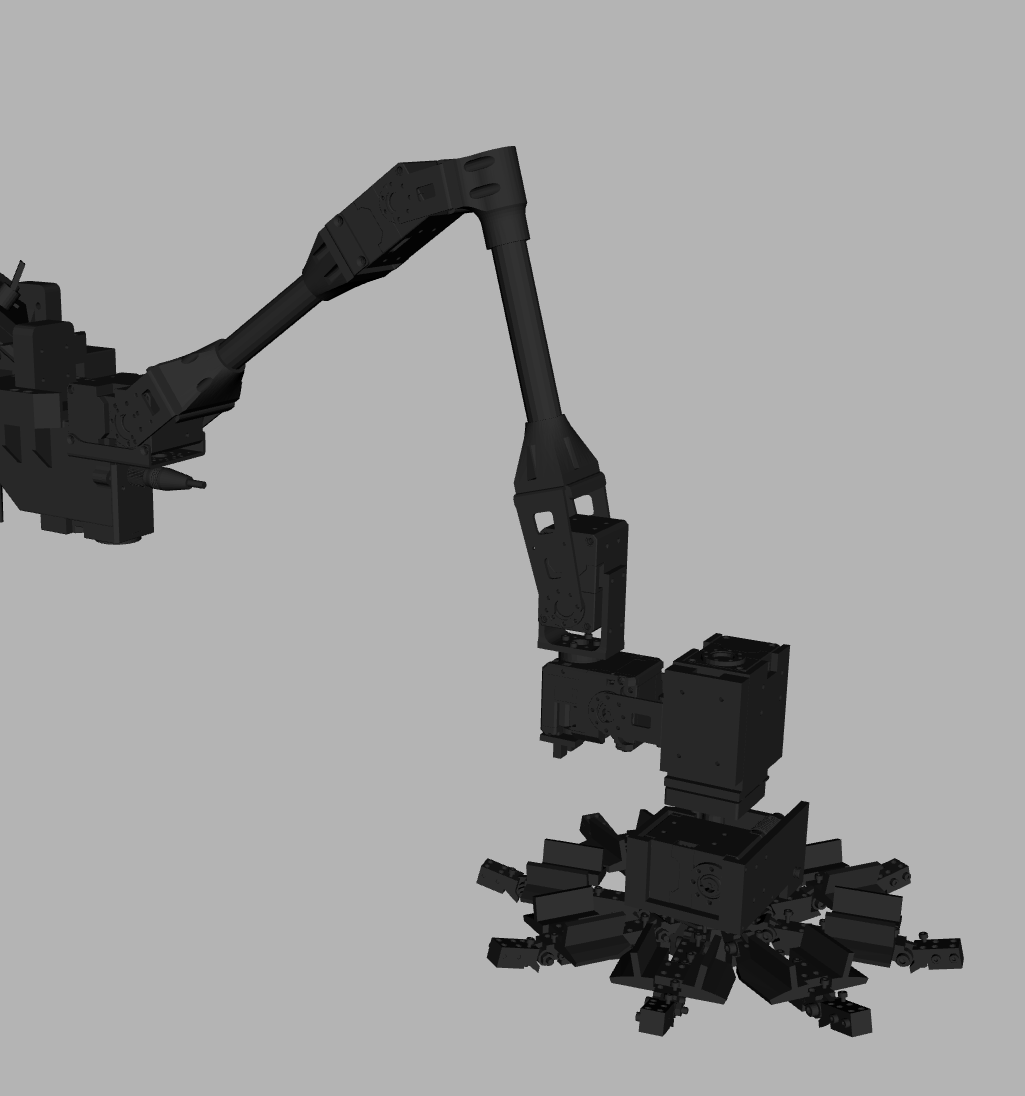
\includegraphics[width=0.4\textwidth]{Images/img_ch4/LIMBERO_GRIEEL_GRIPPER_ortho.png}}   \quad\subfloat[Perspective view in wheel mode.\label{fig:LIMBERO_GRIEEL_WHEEL_ortho}]{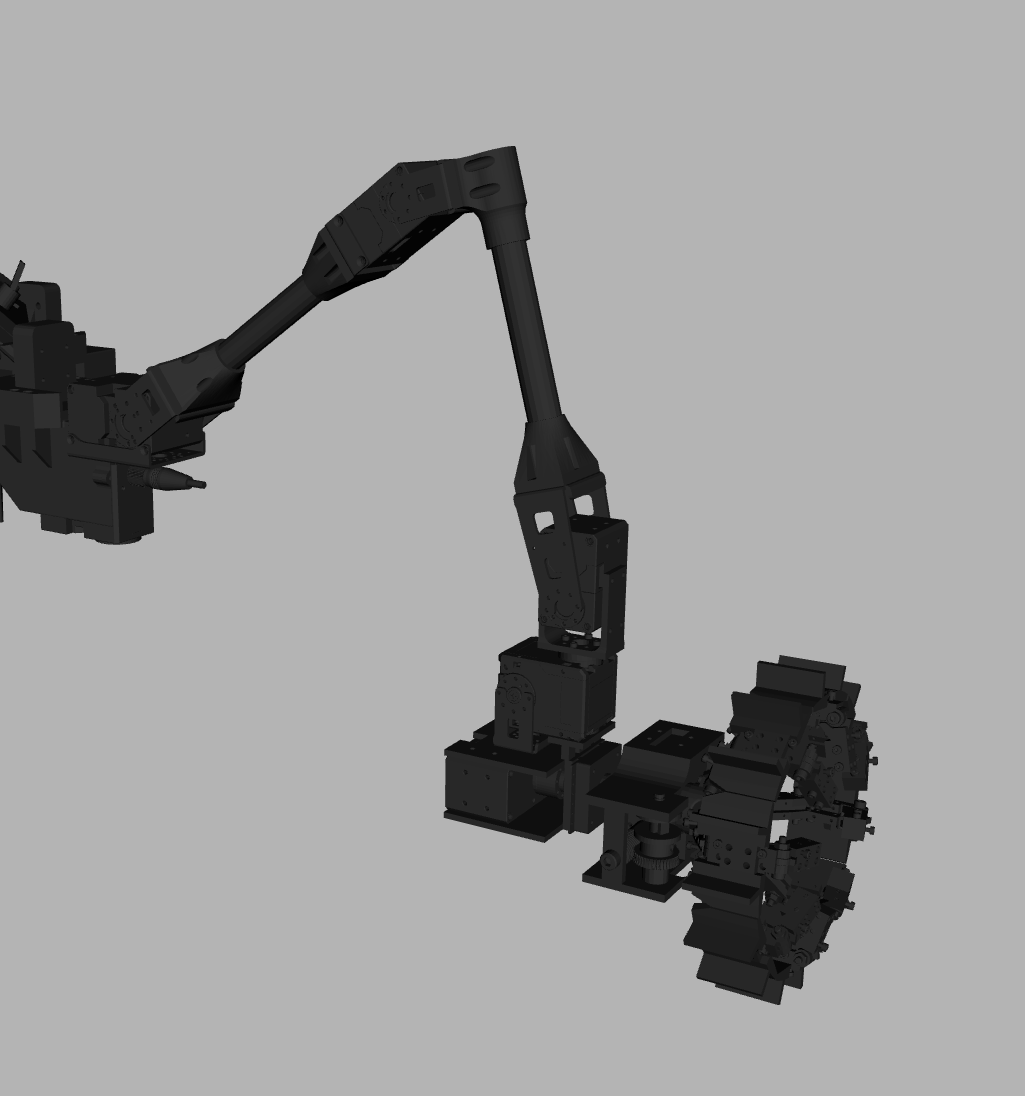
\includegraphics[width=0.4\textwidth]{Images/img_ch4/LIMBERO_GRIEEL_WHEEL_ortho.png}}
    \\
    \subfloat[Real limb in gripper mode. \label{fig:LIMBERO_GRIEEL_GRIPPER_hw}]{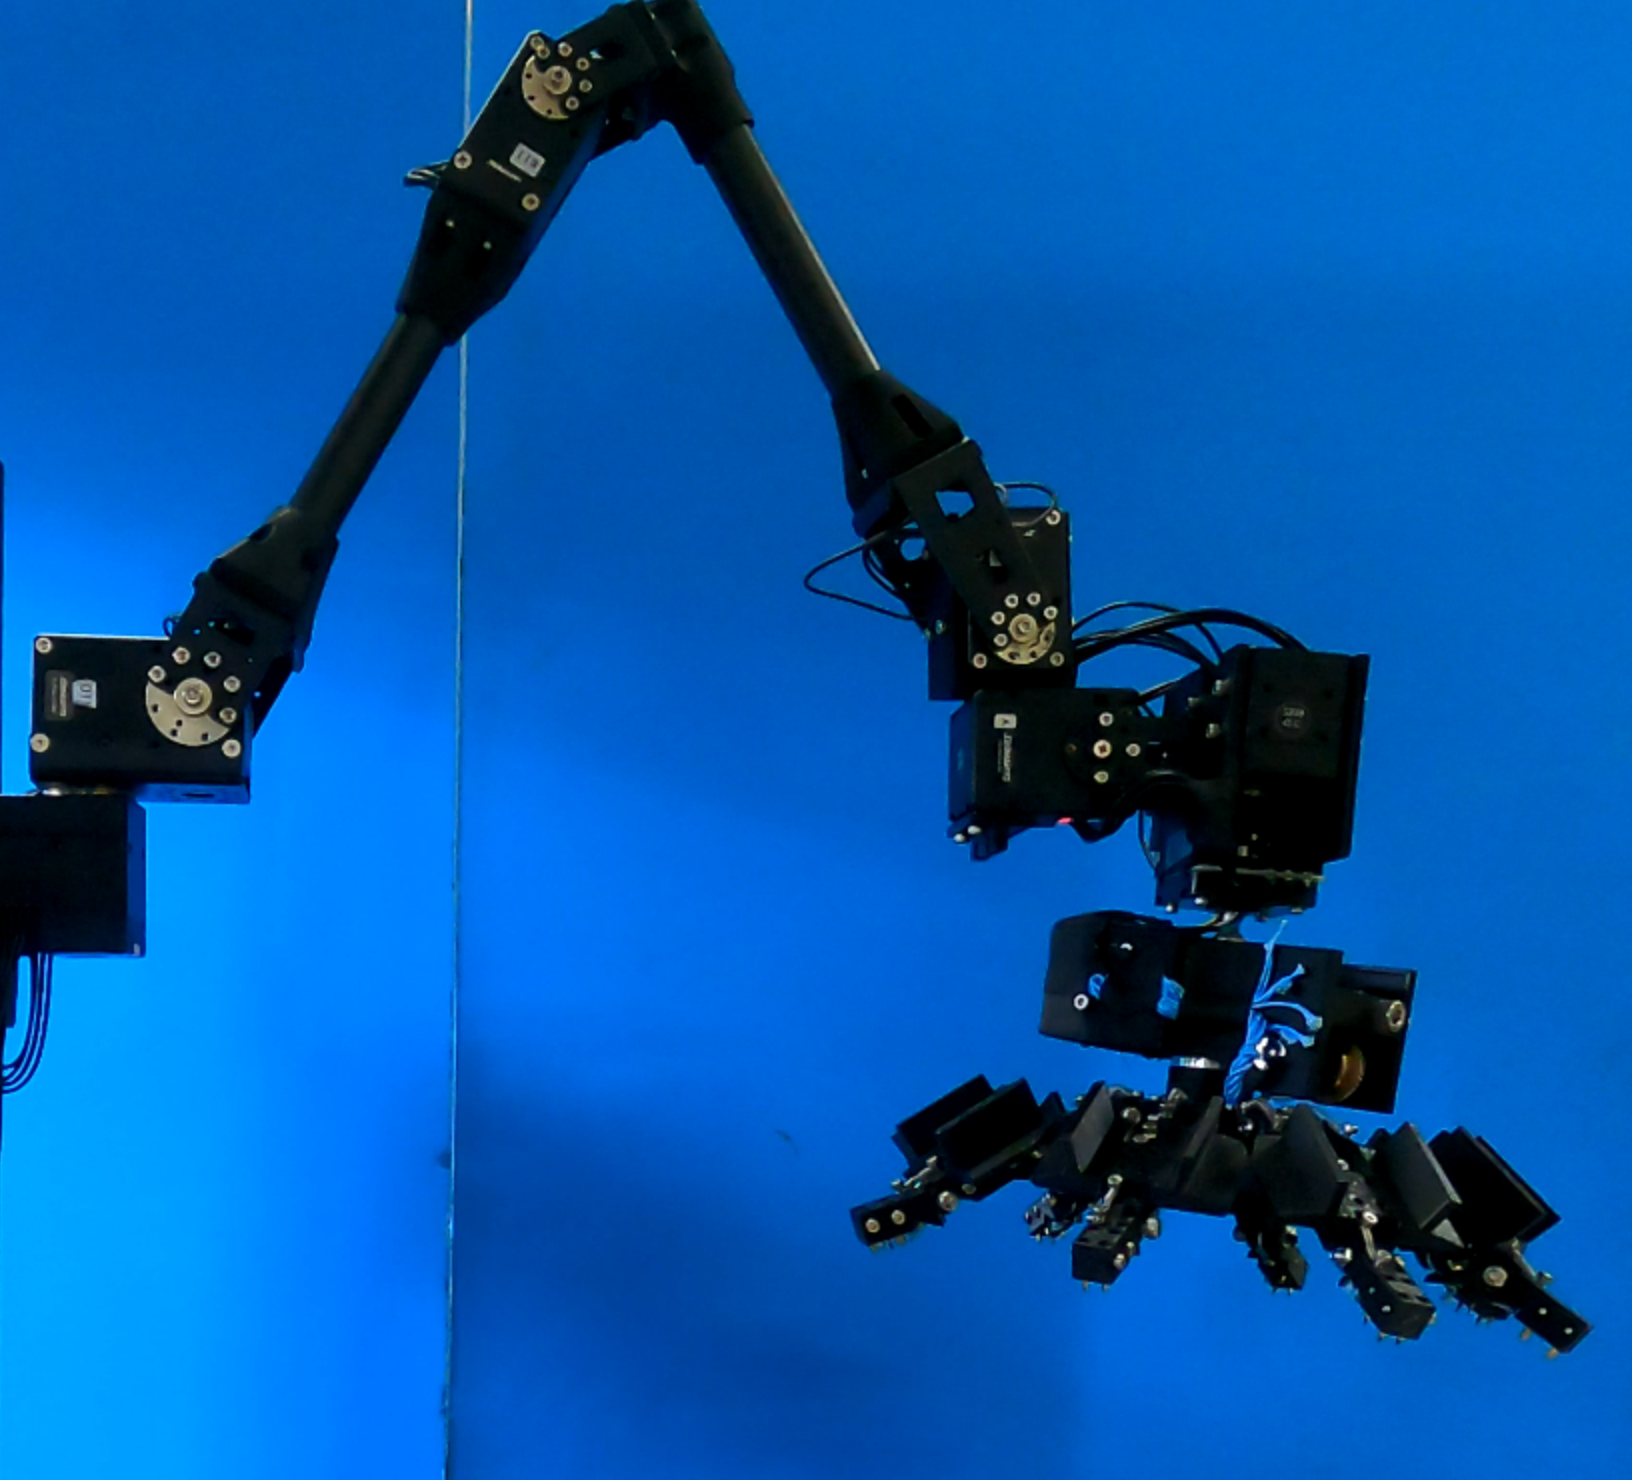
\includegraphics[width=0.4\textwidth]{Images/img_ch4/LIMBERO_GRIEEL_GRIPPER_hw.png}}   \quad\subfloat[Real limb in wheel mode.\label{fig:LIMBERO_GRIEEL_WHEEL_hs}]{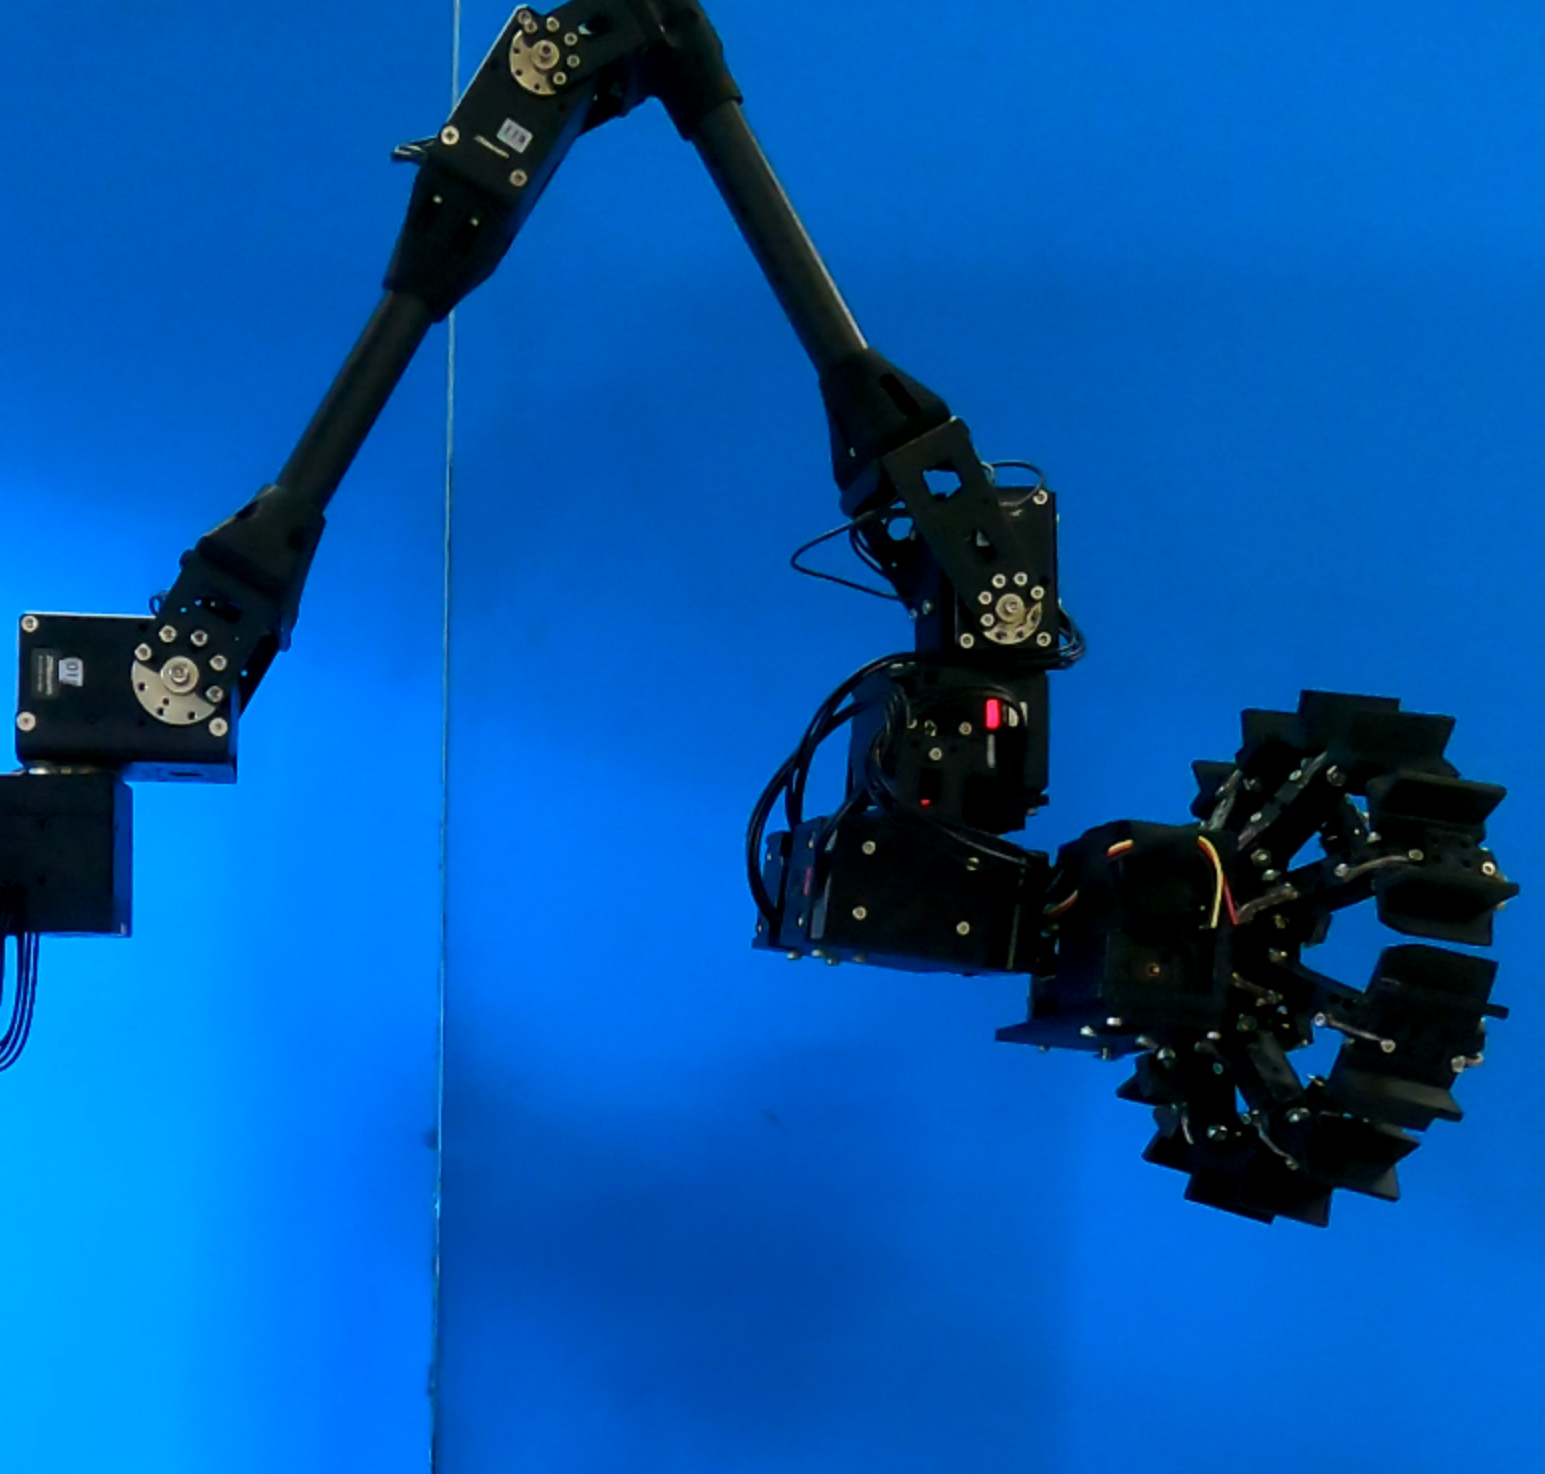
\includegraphics[width=0.4\textwidth]{Images/img_ch4/LIMBERO_GRIEEL_WHEEL_hw.png}}

    \caption[Different views of LIMBERO-GRIEEL limb model and real system]{Different views of LIMBERO-GRIEEL limb model and real system}
    \label{fig:LIMBERO_GRIEEL_limb}
\end{figure}

\begin{figure}[H]
    \centering
    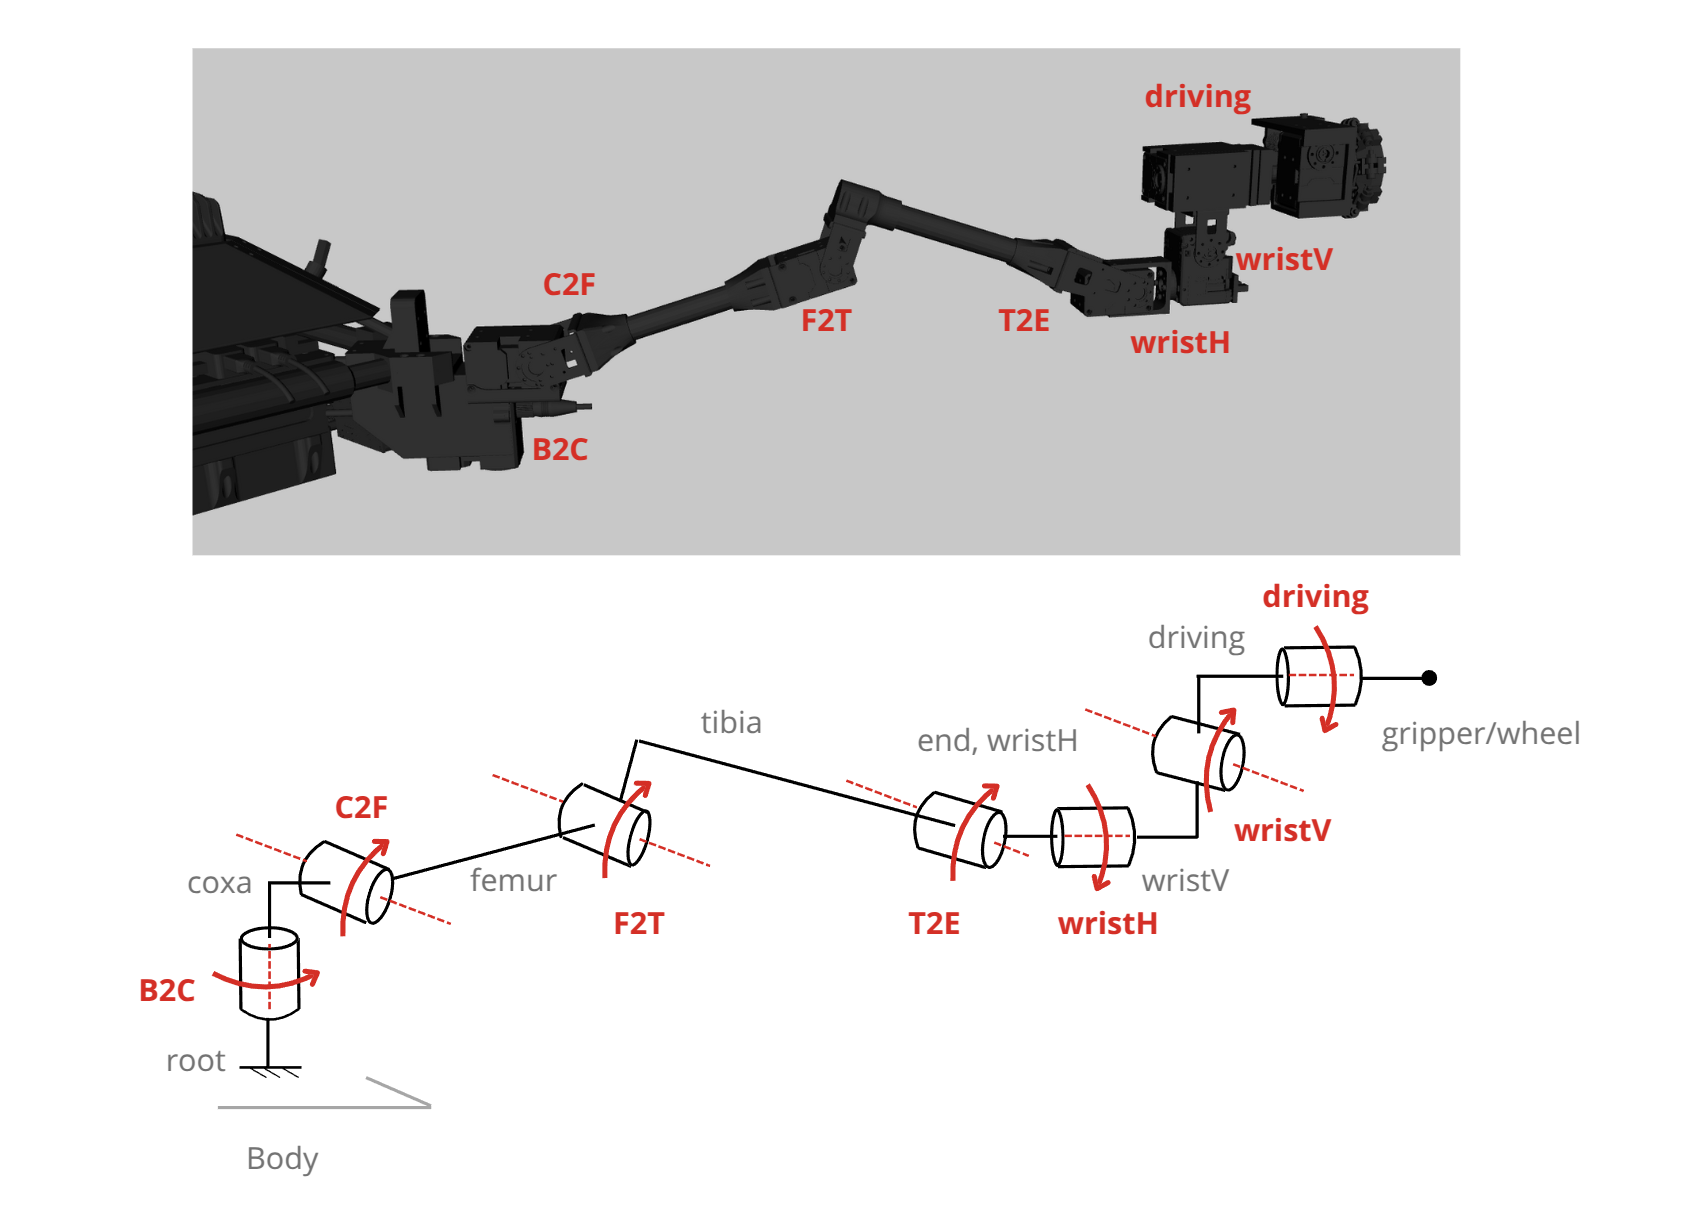
\includegraphics[width=1.0\textwidth]{Images/img_ch4/LIMBERO_GRIEEL_limb_model.png}
    \caption{Schematic model of actuated joints of LIMBERO-GRIEEL limb}
    \label{fig:LIMBERO_GRIEEL_limb_model}
\end{figure}

In principle, in the 3D translational/rotational task space this 7-DOFs structure is redundant, but as evident from the wheel mode, the \textit{driving} joint is included for wheeled locomotion. Therefore, in the motion tasks, the first six joints are used to control the pose, while the last when driving locomotion is required. However, in manipulation task, even when the module is used in gripper mode, the driving motor could be used to change the orientation of the manipulated object, which can be useful in some applications such as pick and place of samples.   

\begin{figure}[H]
    \centering
    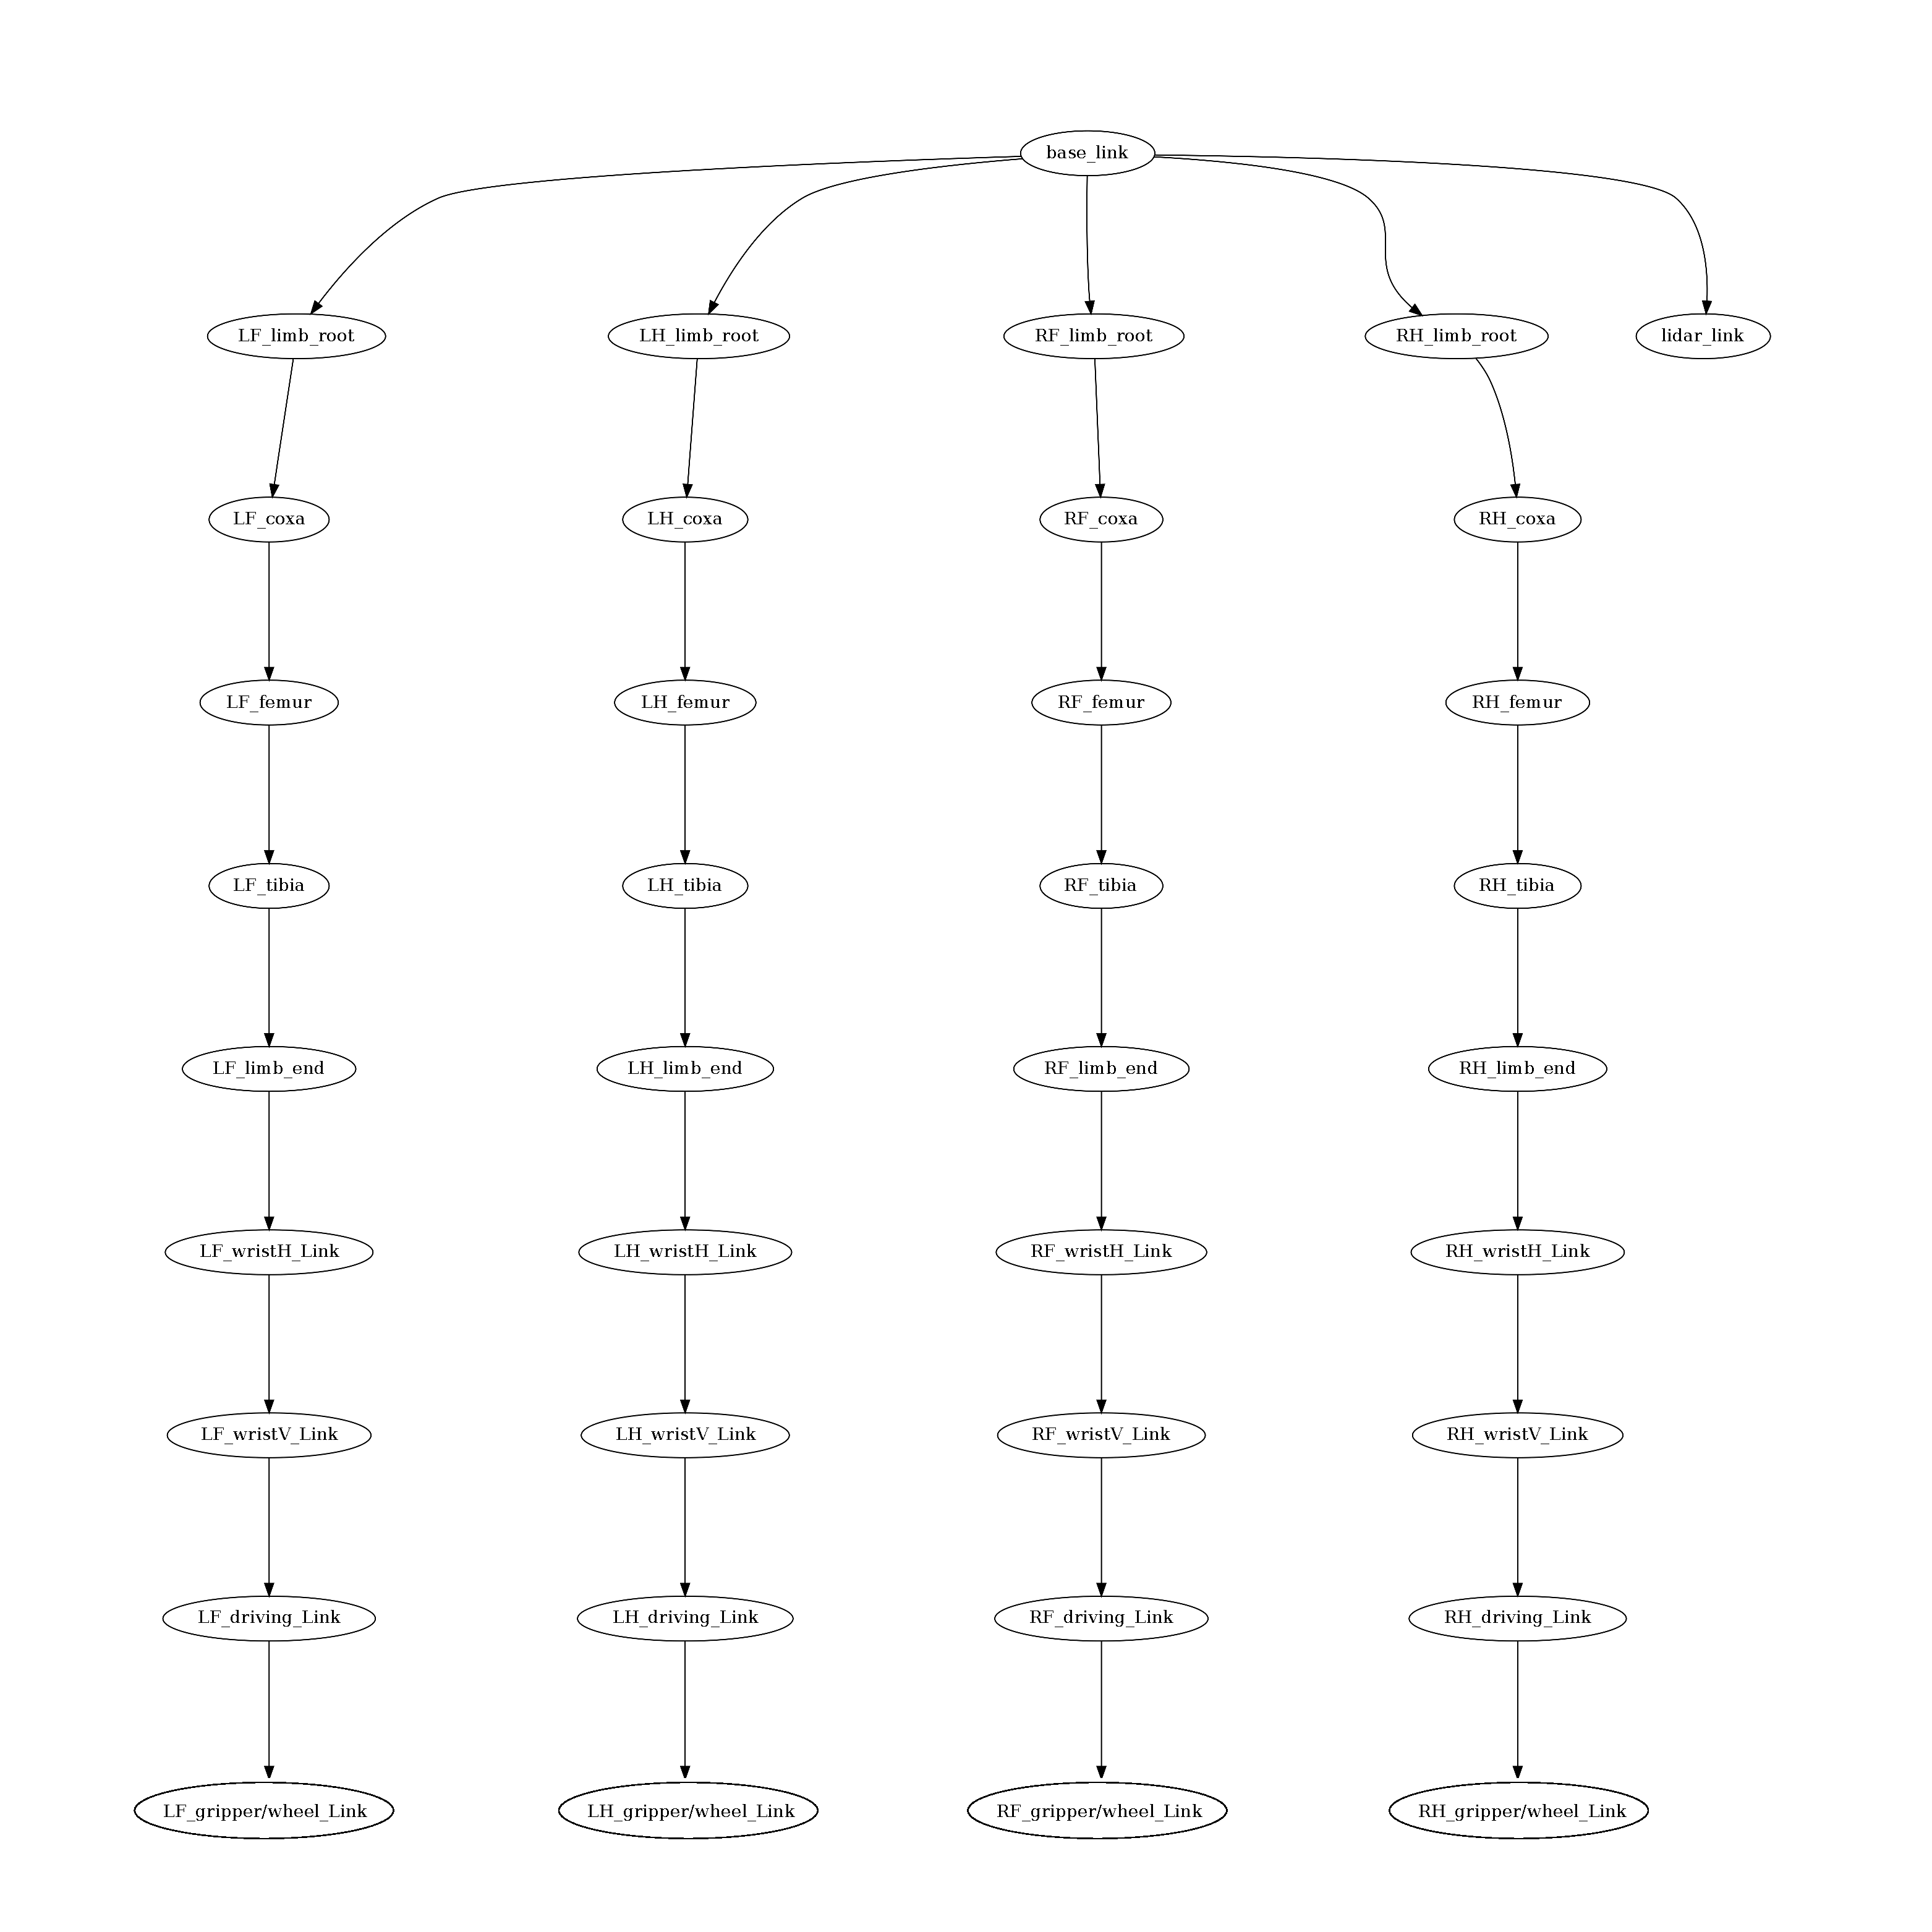
\includegraphics[width=1.0\textwidth]{Images/img_ch4/TFTree_NOFINGERS.pdf}
    \caption{Links structure of LIMBERO-GRIEEL Limb, neglecting gripper-wheel transformation fingers' joints}
    \label{fig:TFTree_NOFINGERS}
\end{figure}

Finally, the equivalent DH model of the limb is represented in Fig.\ref{fig:limbero_grieel_DH} (extracted from the robot Unified Robot Description Format (URDF), described in the software section), the DH parameters are reported in Tab.\ref{table:DH}, and the value of masses in Tab.\ref{table:Mass}.

\begin{table}[H]
\centering 
    \caption{LIMBERO-GRIEEL DH parameters}
    \label{table:DH}
    \begin{tabular}{| l | c | c | c | c | c |}
    \hline
    \rowcolor{bluepoli!40}
%    \rowcolor{bluepoli!40}
     \textbf{Link} &  $a_i$ $[m]$ & $\alpha_i$ $[rad]$ & $d_i$ $[m] $ & $\theta_i$ $[rad]$ & $\theta_{offset, i}$ $[rad]$ \T\B \\
    \hline \hline
    \textbf{coxa} ($i=1$) & 0.031 & $-\frac{\pi}{2}$ & 0.0  & $q_1$  & 0.0 \T\B\\
    \hline 
    \textbf{femur} ($i=2$) & 0.2 & 0.0  & 0.0  & $q_2$  & 0.0  \T\B\\
    \hline
    \textbf{tibia} ($i=3$) & 0.2  & 0.0  & 0.0  & $q_3$ & 0.0 \T\B\\
    \hline
    \textbf{limb-end} ($i=4$) & 0.0 &  $-\frac{\pi}{2}$ & 0.0 & $q_4$ &  $-\frac{\pi}{2}$  \B\\
    \hline
    \textbf{wristV} ($i=5$) & 0.024 &  $\frac{\pi}{2}$ & 0.0468 & $q_5$  & 0.0 \B\\
    \hline
    \textbf{driving} ($i=6$) & 0.0458  &  $-\frac{\pi}{2}$ & 0.0 & $q_6$  &  0.0 \B\\
    \hline
    \textbf{gripper/wheel} ($i=7$) & 0.0 & 0.0 & 0.1131 & $q_7$ & 0.0   \B\\
    \hline
    \end{tabular}

\end{table}

\begin{table}[H]
    \caption{LIMBERO-GRIEEL links masses}
    \label{table:Mass}
     \hspace{-2.0cm} % Adjust this value as needed
    \begin{tabular}{| c || l | l | l | l | l | l | l | l | l | l |}
    \hline
     \cellcolor{bluepoli!40}\textbf{Link} & body & root  & coxa & femur & tibia & limb-end & wristH & wristV & driving & G/W \T\B \\
    \hline 
    \cellcolor{bluepoli!40}\textbf{mass} [kg] & 3.115  & 0.085 & 0.091 &  0.128 & 0.062 & 0.082 & 0.008 & 0.102 & 0.133 & 0.416\T\B\\
    \hline 
    \end{tabular}
\end{table}

\begin{figure}[H]
    \centering
    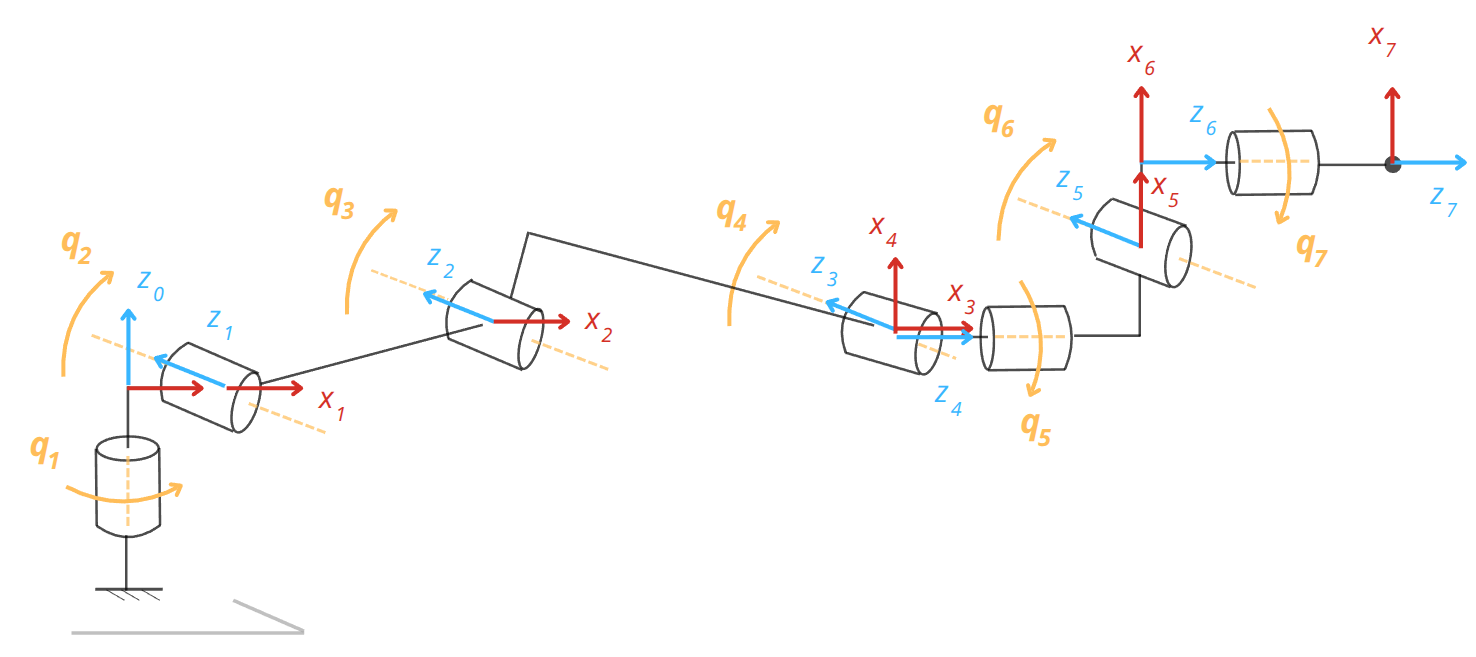
\includegraphics[width=0.8\textwidth]{Images/img_ch4/limbero_grieel_DH.png}
    \caption{LIMBERO-GRIEEL links and joints scheme with DH convention}
    \label{fig:limbero_grieel_DH}
\end{figure}

The overall LIMBERO-GRIEEL robot, composed of 4 limbs (LF,LH,RH,RF) with the structure described above, attached to a base, is reported in Fig.\ref{fig:LIMBERO_GRIEEL_robot} and Fig.\ref{fig:robot_LIMBERO_GRIEEL_GRIPPER_hw_front} below. 
\begin{figure}[H]
    \centering
    \subfloat[Gripper mode\label{fig:robot_LIMBERO_GRIEEL_GRIPPER_hw}]{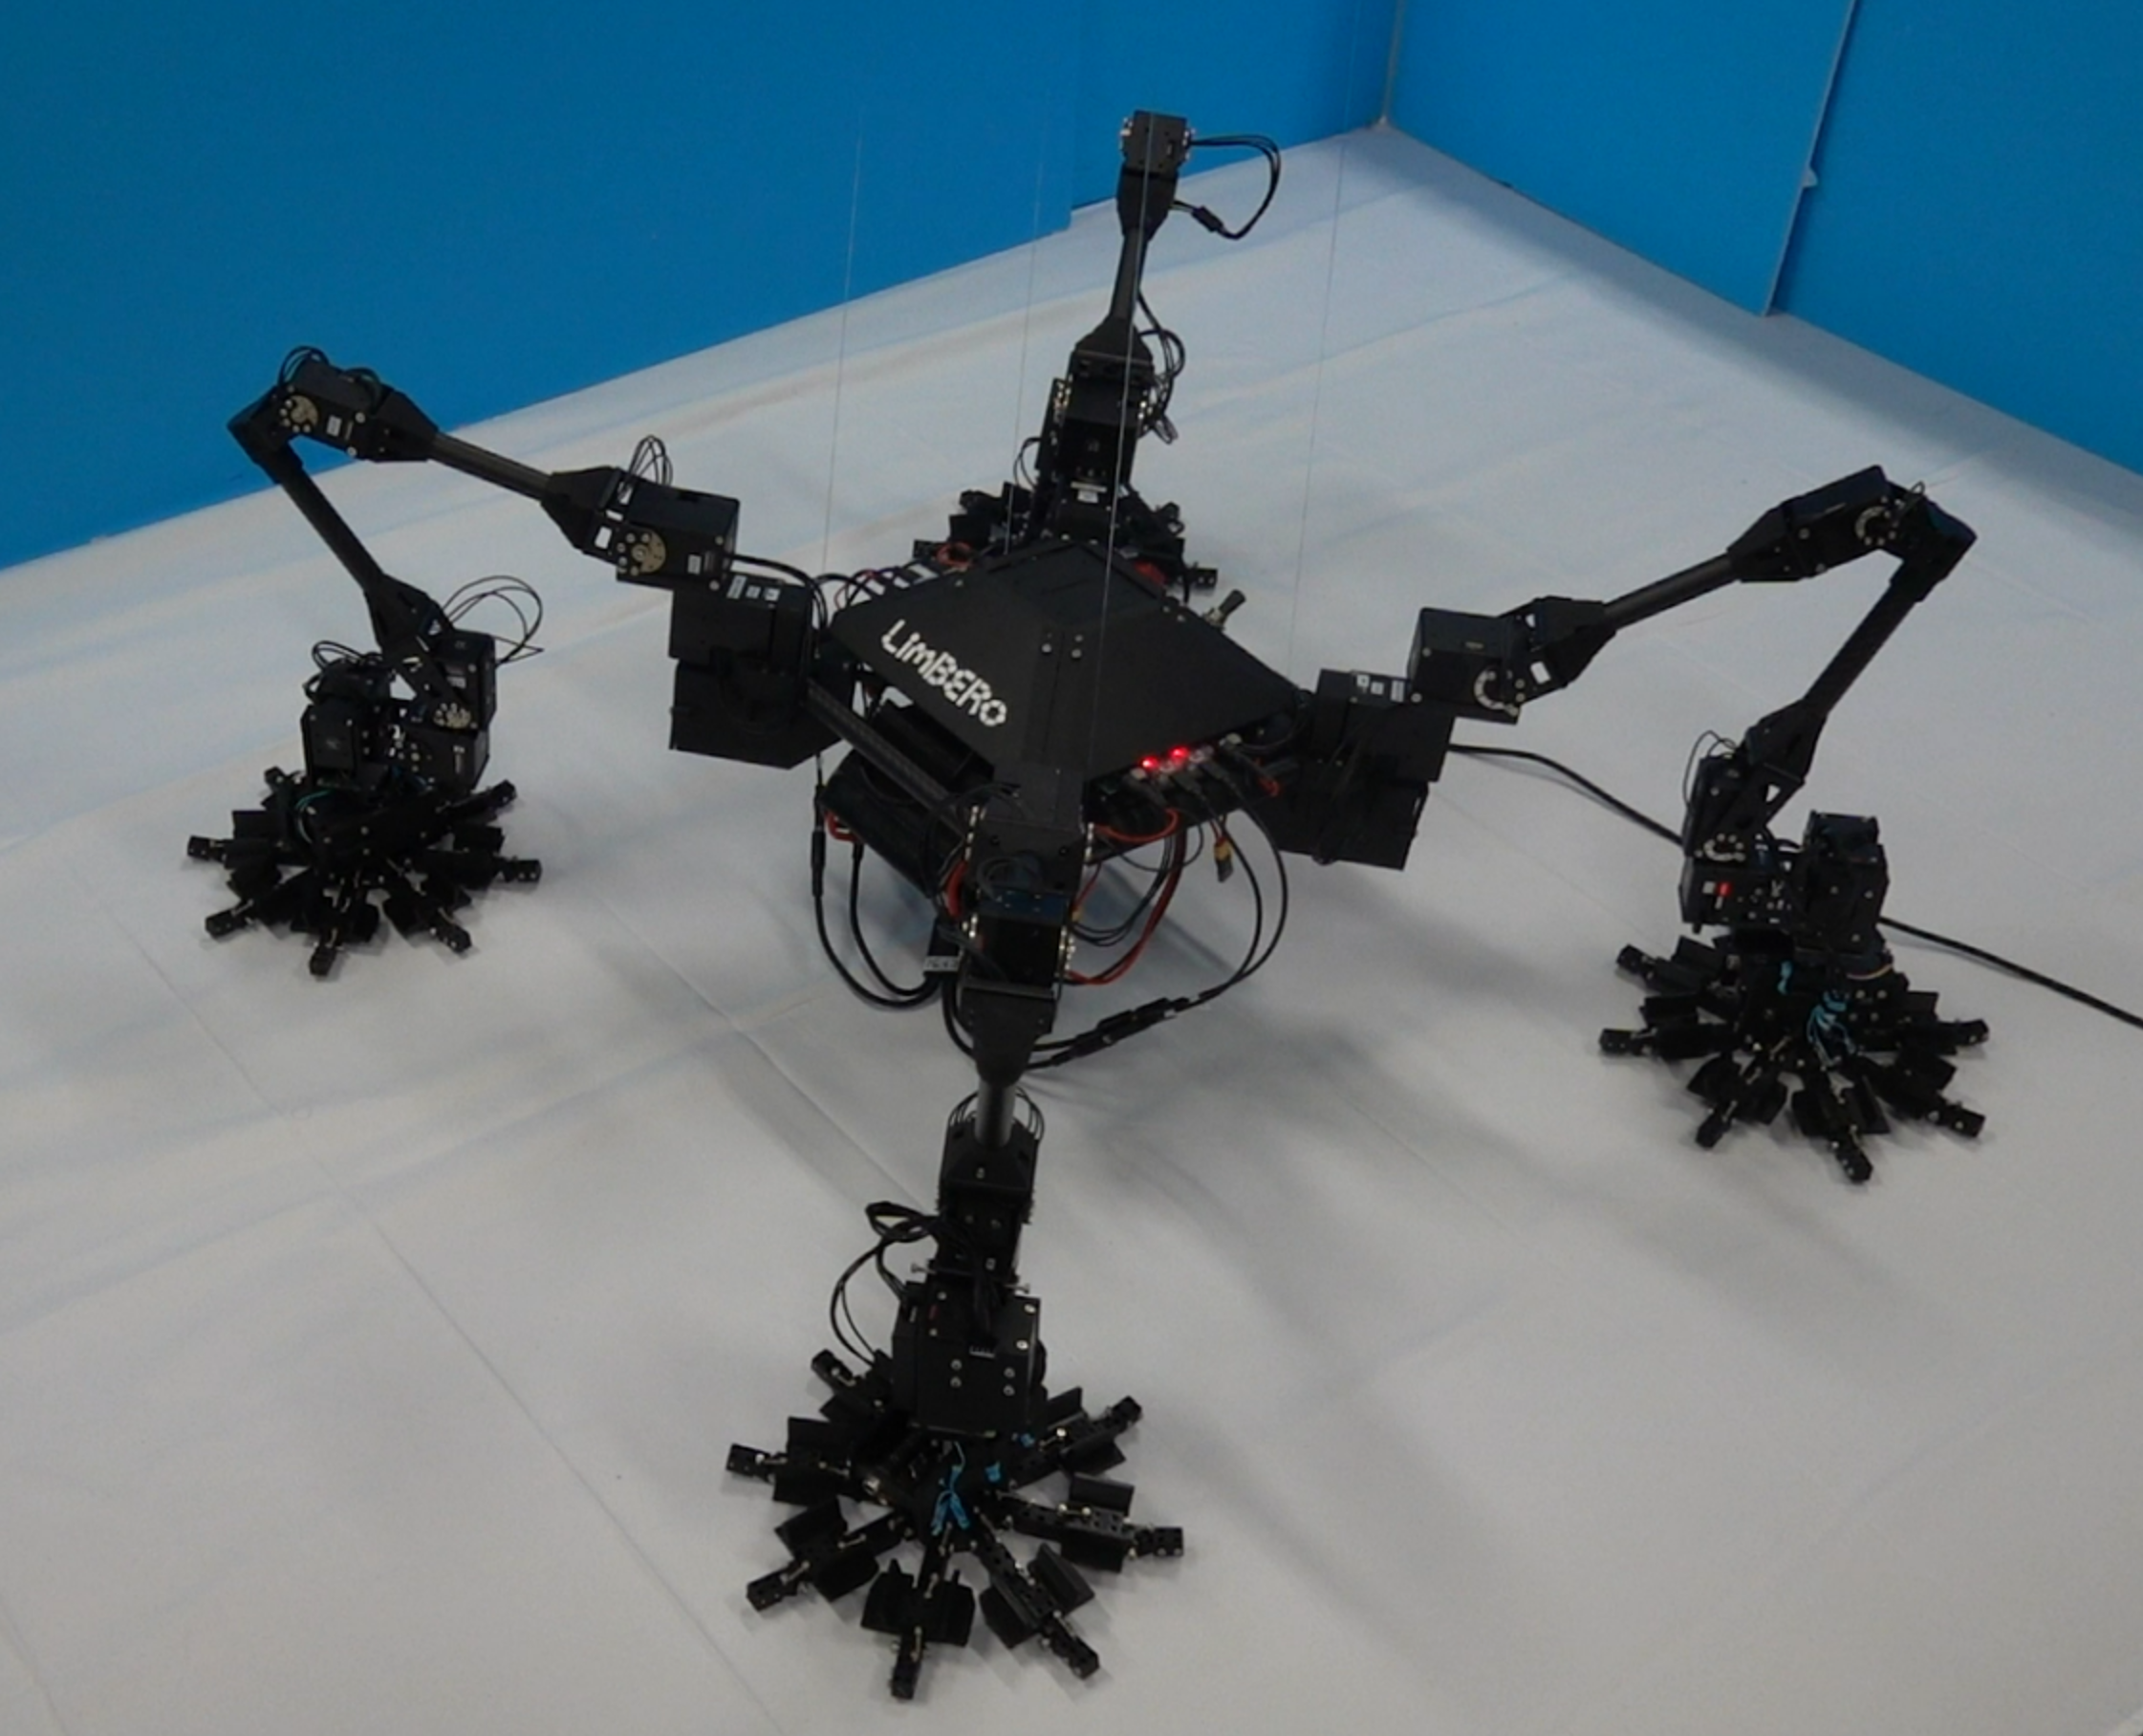
\includegraphics[width=0.35\textwidth]{Images/img_ch4/robot_LIMBERO_GRIEEL_GRIPPER_hw.png}} \quad 
    \subfloat[Wheel mode\label{fig:robot_LIMBERO_GRIEEL_WHEEL_hw}]{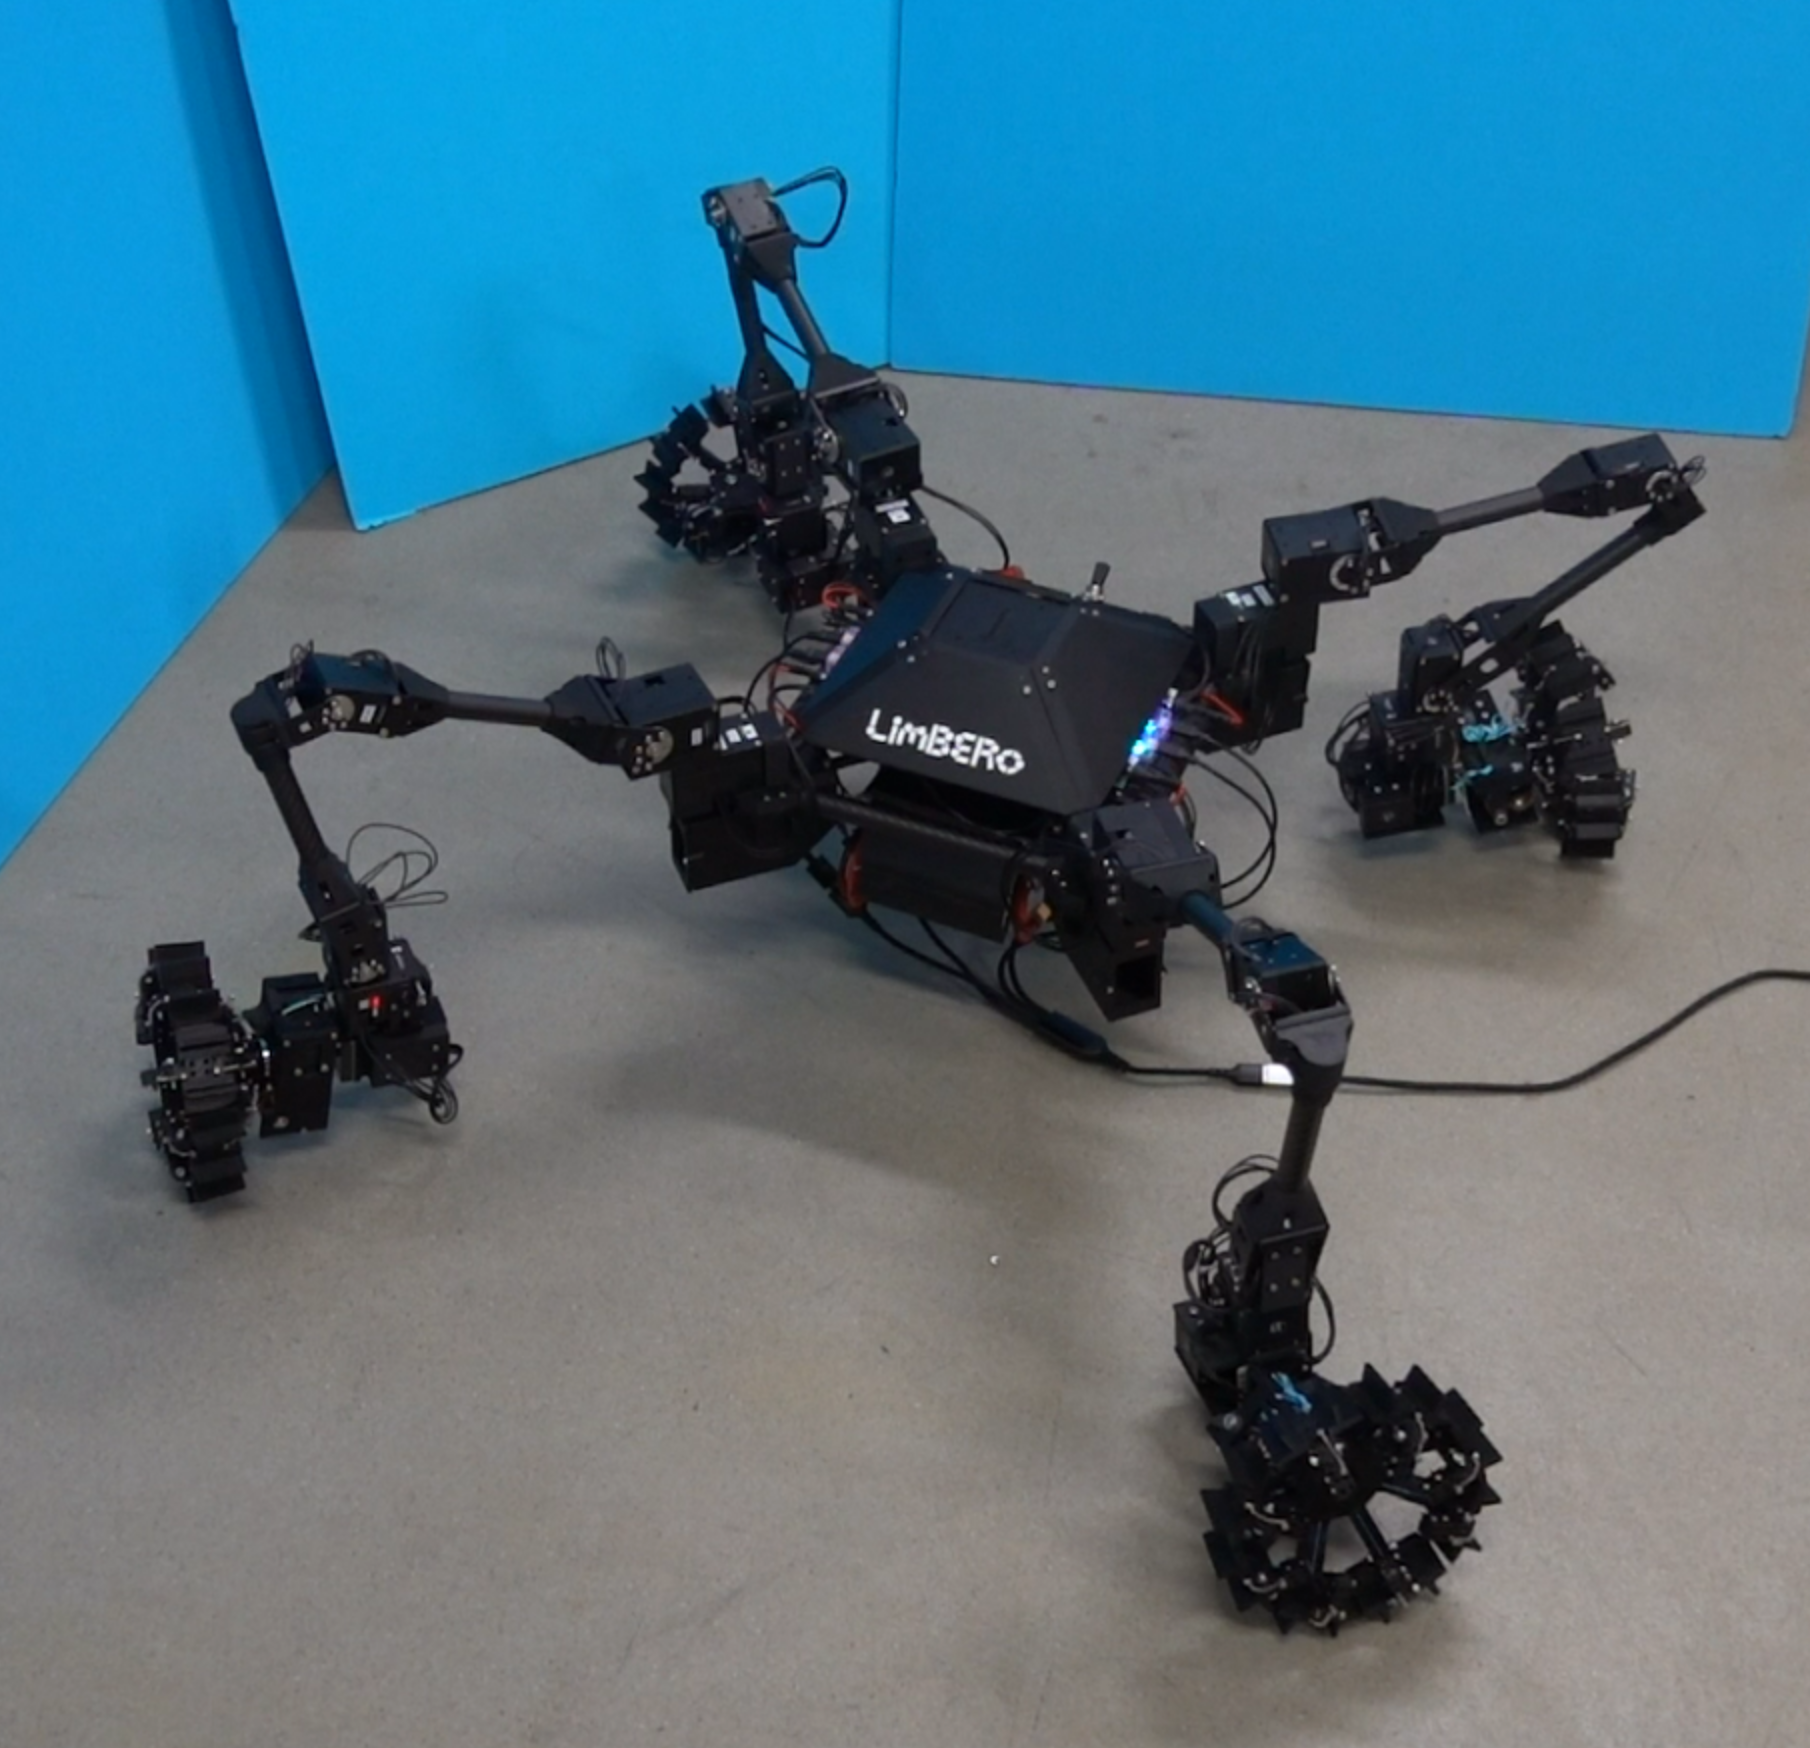
\includegraphics[width=0.3\textwidth]{Images/img_ch4/robot_LIMBERO_GRIEEL_WHEEL_hw.png}} 
    \caption[LIMBERO-GRIEEL robot]{LIMBERO-GRIEEL robot in wheel and gripper mode}
    \label{fig:LIMBERO_GRIEEL_robot}
\end{figure}

\begin{figure}[H]
    \centering
    \subfloat[Gripper mode front view \label{fig:robot_LIMBERO_GRIEEL_GRIPPER_hw_front}]{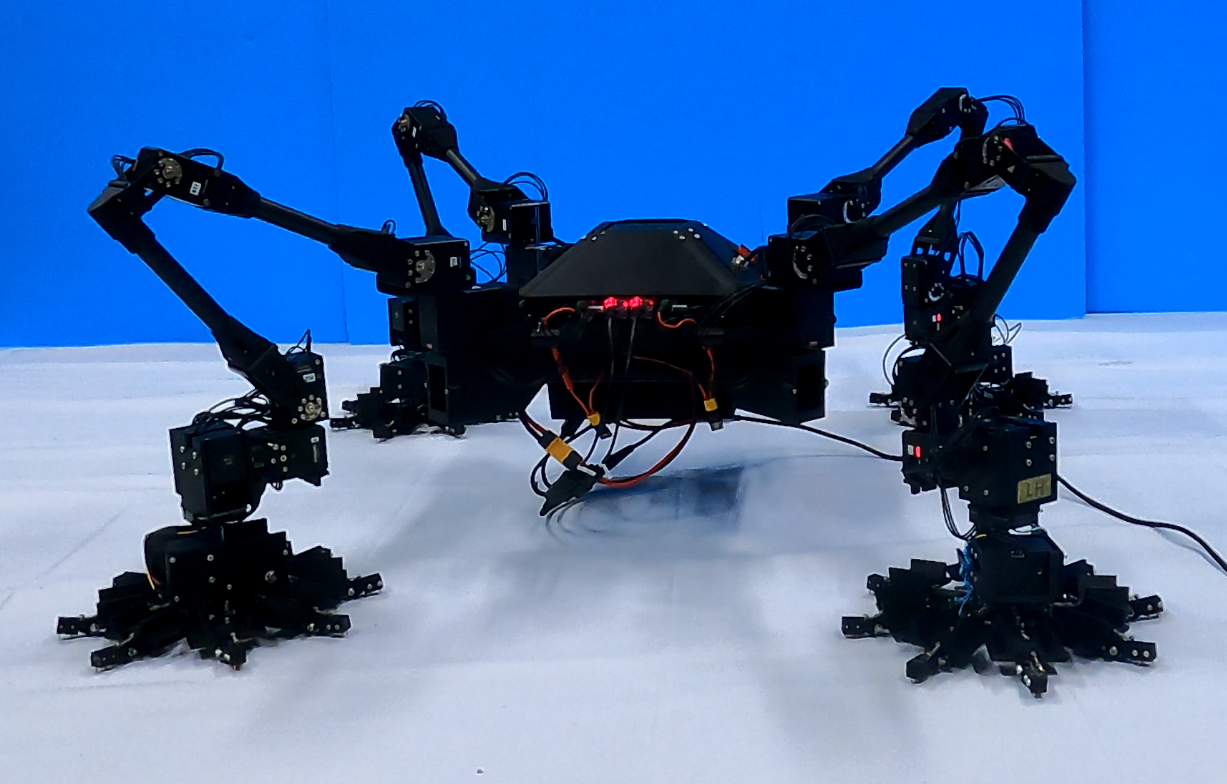
\includegraphics[width=0.35\textwidth]{Images/img_ch4/GripperMode_Front.png}} \quad 
    \subfloat[Wheel mode front view\label{fig:robot_LIMBERO_GRIEEL_WHEEL_hw_front}]{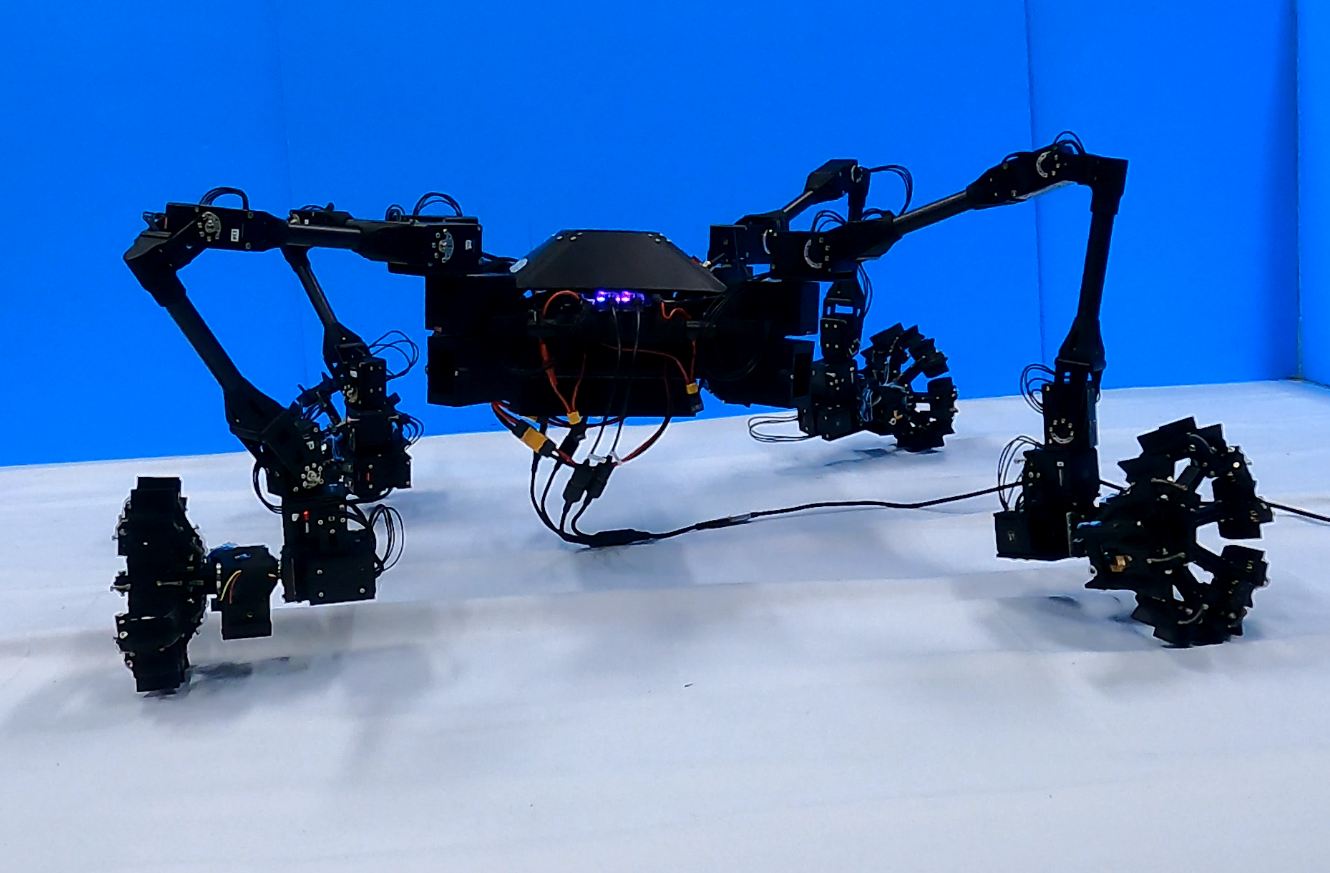
\includegraphics[width=0.35\textwidth]{Images/img_ch4/WheelMode_Front.png}} 

    \caption[LIMBERO-GRIEEL robot in wheel and gripper mode]{LIMBERO-GRIEEL robot in wheel and gripper mode}
    \label{fig:LIMBERO_GRIEEL_robot_front}
\end{figure}


This description of the limbs' joints and links neglects the DOFs used by the gripper-wheel mechanism for transformation, now considered as a single rigid body.
Next, the process of the transformation is briefly described, providing a complete model useful for simulation. 

\subsection{Gripper-Wheel Transformation}
\label{sec:gripper_wheel}

The final mechanism assembled and patented by M.Uda \cite{GrieelUda}\cite{GrieelUda} comes from the following design requirements:
\begin{enumerate}
    \setlength\itemsep{-0.7em} 
    \item Ability to switch between gripper and wheel at will.
    \item Ability to maintain sufficient grip on uneven terrain and steep slopes. 
    \item High driving performance. 
\end{enumerate}

The system is composed of eight fingers in an equally spaced radial disposition around a central "hand", each finger has four links, interconnected by passive rotational joints with springs and an internal tether. Each finger's tip has for claws for gripping capabilities, widely tested during prototyping.
As represented in Fig.\ref{fig:Gripper_Wheel}, the mechanism is in gripper mode when all fingers are opened, and in wheel mode when closed. The Transformation from gripper to wheel (G2W) is achieved by pulling all the tethers, which are connected to a single servo motor, with a locking function achieved using a worm gear. 
The opposite mode transformation (W2G) instead releases the tethers rotating the servo motor in the opposite direction and exploits the restoring force of the springs to open the fingers. A schematic view of the closing sequence for one finger is represented in Fig.\ref{fig:closing_finger}, while the real finger design and overall mechanism with the transforming servo motor is in Fig.\ref{fig:Gripper_Wheel_mechanism}.

The servo motor used to open and close the mechanism is not included in the joint space of the limb because it doesn't contribute to the positioning of the EE, but to the locomotion change. Considering a single finger, the palm is considered as part of the central hand link, denoting the links as {phalanx1, phalanx2, phalanx3}, and the passive joints as $\{H2P1,\; P12P2,\; P22P3\} = \{\theta_1, \theta_2, \theta_3\} $. The springs are chosen with a spring constant such that, the mimic behavior of the finger joints respects the following constraints:
\begin{equation}
    \label{eq:finger_contraint}
    \left\{
    \begin{aligned}
           \theta_2 = 2\cdot\theta_1  \\
            \theta_3 = 3\cdot\theta_1
    \end{aligned}
    \right.
\end{equation}
With those constraints, in closing finger configuration 
$\theta_1 = \frac{\pi}{6}\;,  \theta_2 = \frac{\pi}{3} \;, \theta_3 = \frac{\pi}{2}$, exactly as represented in Fig.\ref{fig:closing_finger}, and the connection of the eight tethers in the central mechanism guarantee the coordination of all fingers motion (imposing the additional constraint that each finger $\theta_1$ is equal. 

\begin{figure}[H]
    \centering
    \subfloat[\label{fig:closing_finger1}]{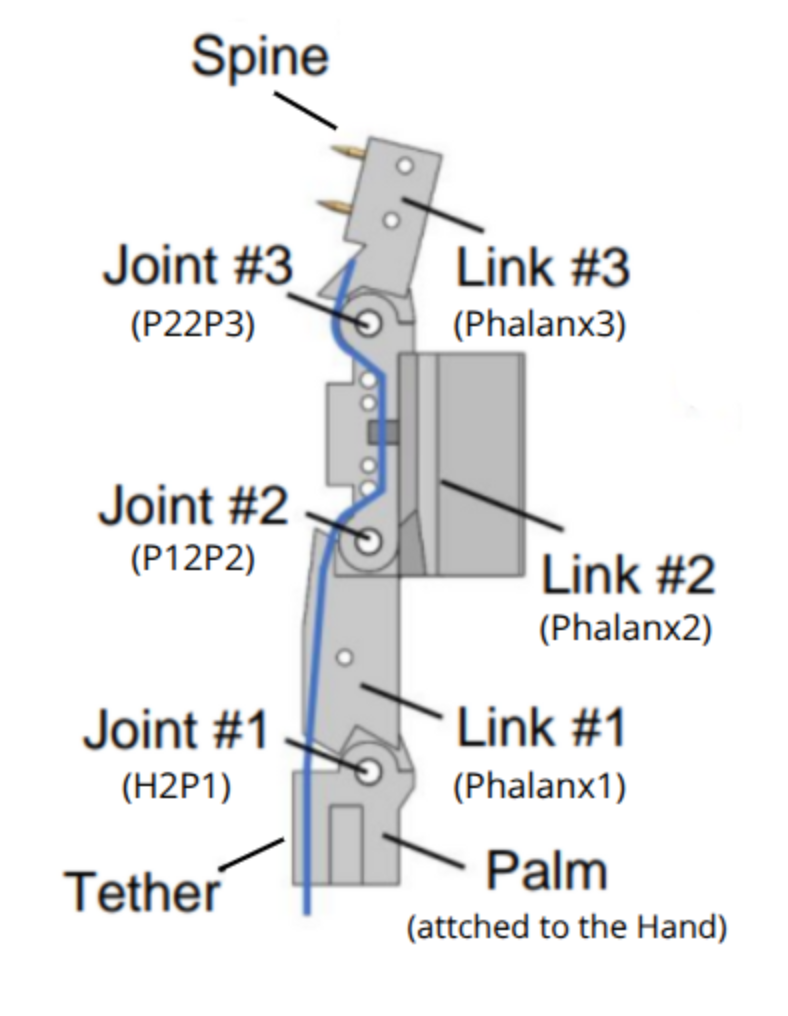
\includegraphics[scale=0.15]{Images/img_ch4/closing_finger1.png}}
    \subfloat[\label{fig:closing_finger2}]{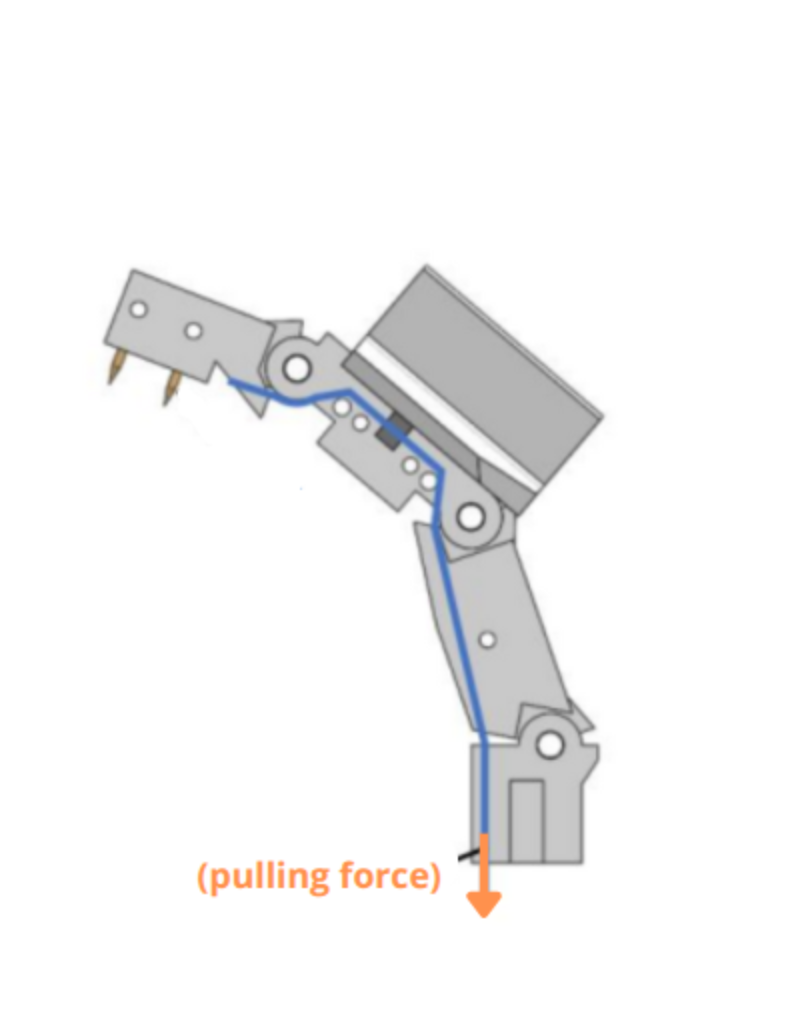
\includegraphics[scale=0.15]{Images/img_ch4/closing_finger2.png}}
    \subfloat[\label{fig:closing_finger3}]{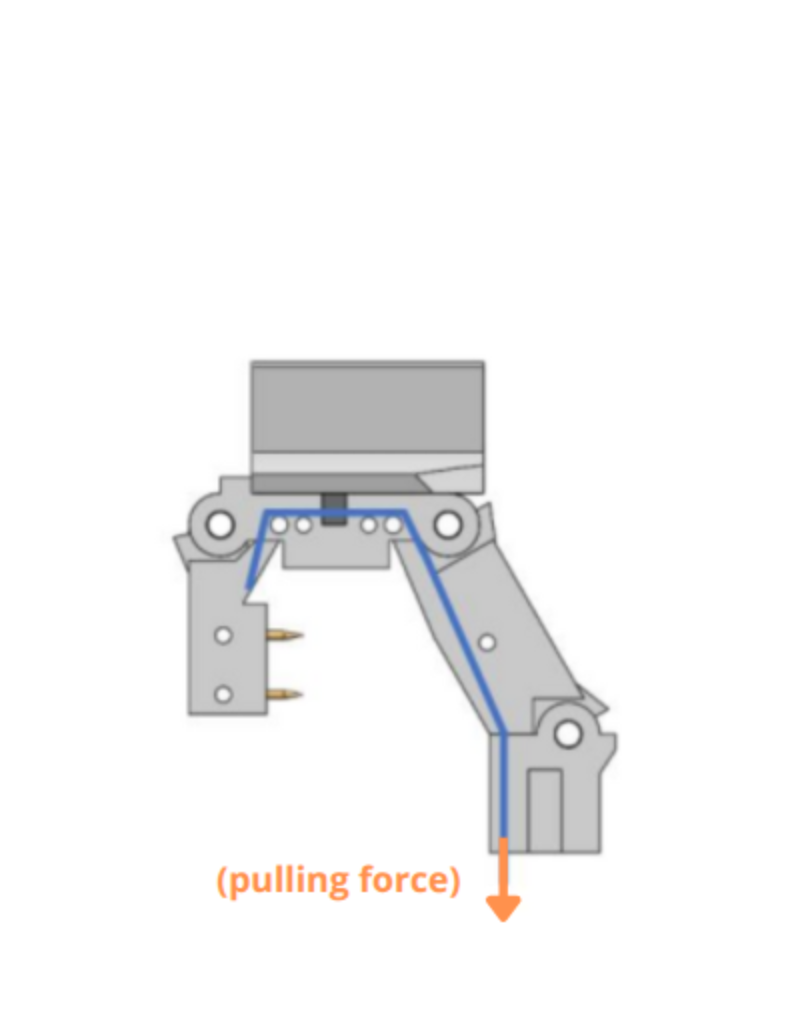
\includegraphics[scale=0.15]{Images/img_ch4/closing_finger3.png}}
    \caption[gripper-wheel mechanism G2W finger sequence]{\cite{GRIEELUdaThesis} representation of single finger closing sequence for G2W transformation: (a) open (Gripper),(b) in transition, (c) closed state (Wheel)}
    \label{fig:closing_finger}
\end{figure}
    

\begin{figure}[H]
    \centering
    \subfloat{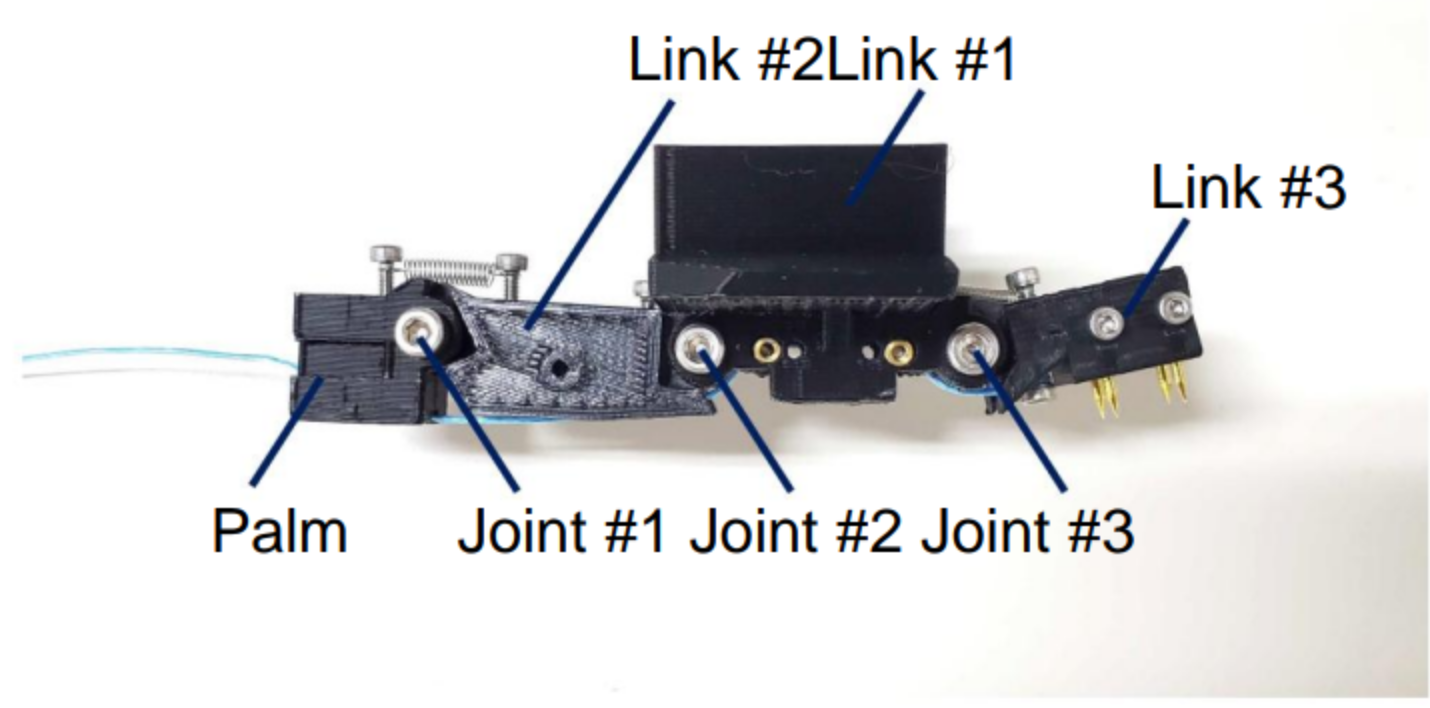
\includegraphics[width=0.4\textwidth]{Images/img_ch4/Gripper_Wheel_mechanism_finger.png}}\quad
    \subfloat{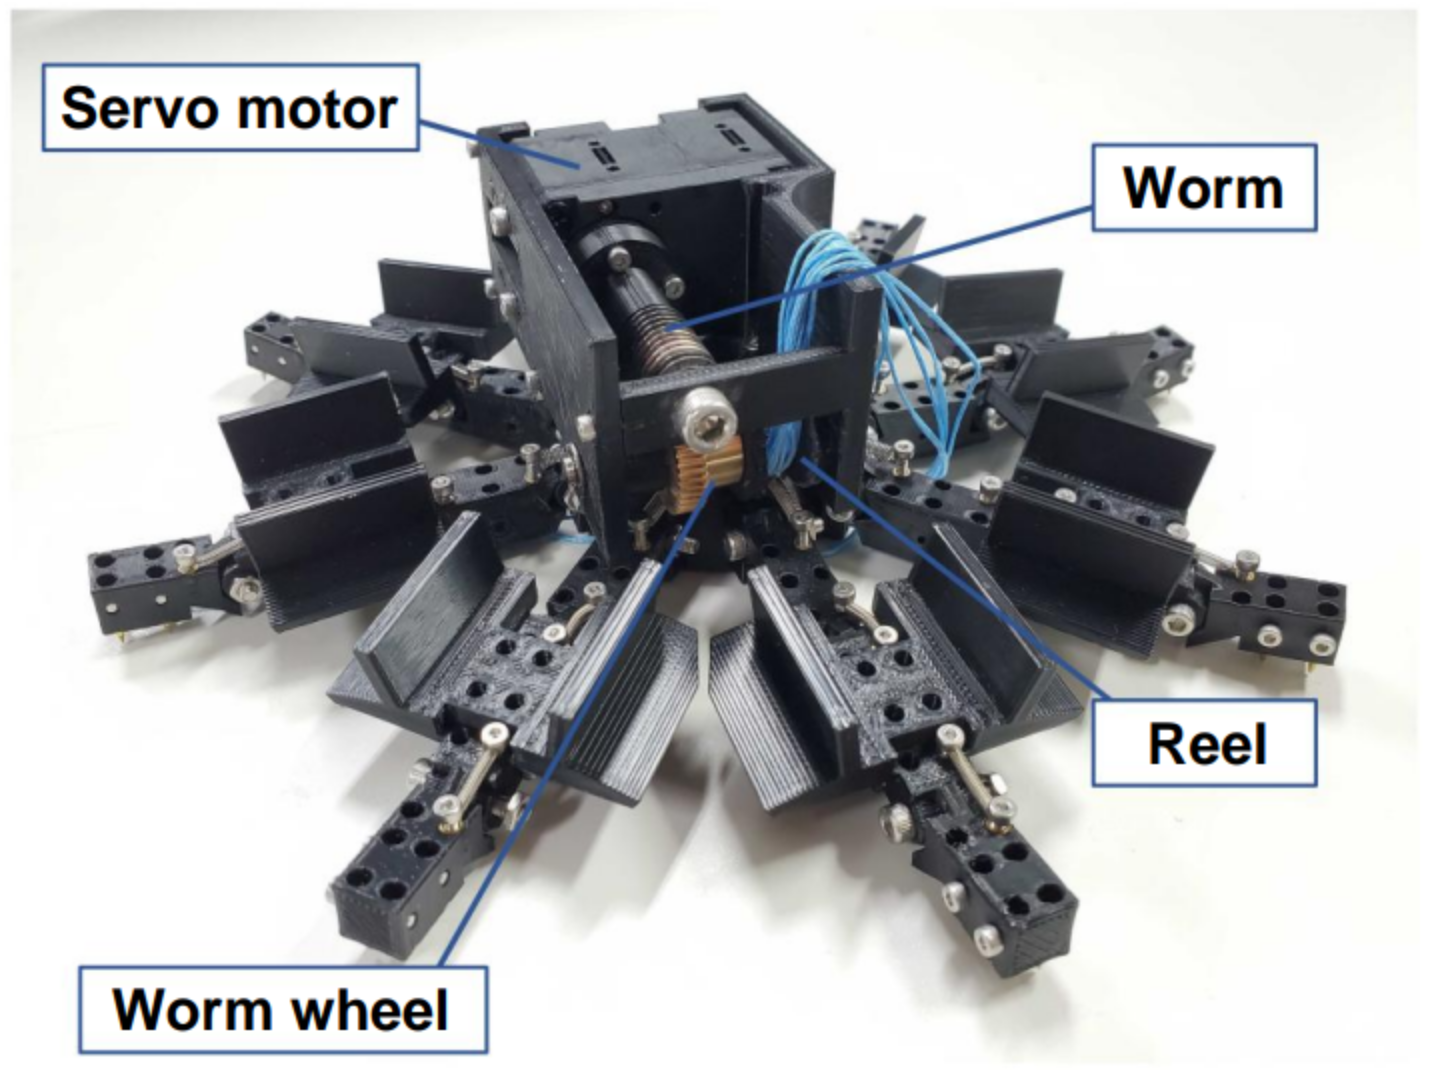
\includegraphics[width=0.4\textwidth]{Images/img_ch4/Gripper_Wheel_mechanism_all.png}}
    \caption[Single Finger and overall gripper-wheel mechanism]{\cite{GRIEELUdaThesis} Finger and overall gripper-wheel mechanism}
    \label{fig:Gripper_Wheel_mechanism}
\end{figure}

Expanding the notation to consider all the fingers of one mechanism,\\ the prefix $j\_Fk\_<link>$ is used to represent $j^{th}$ limb $k^{th}$ finger, and Fig.\ref{fig:TFTree_FINGERS} describes the mechanism links and passive joints interconnection tree, with the mimic constraint defined above. 

\begin{figure}[H]
    \centering
    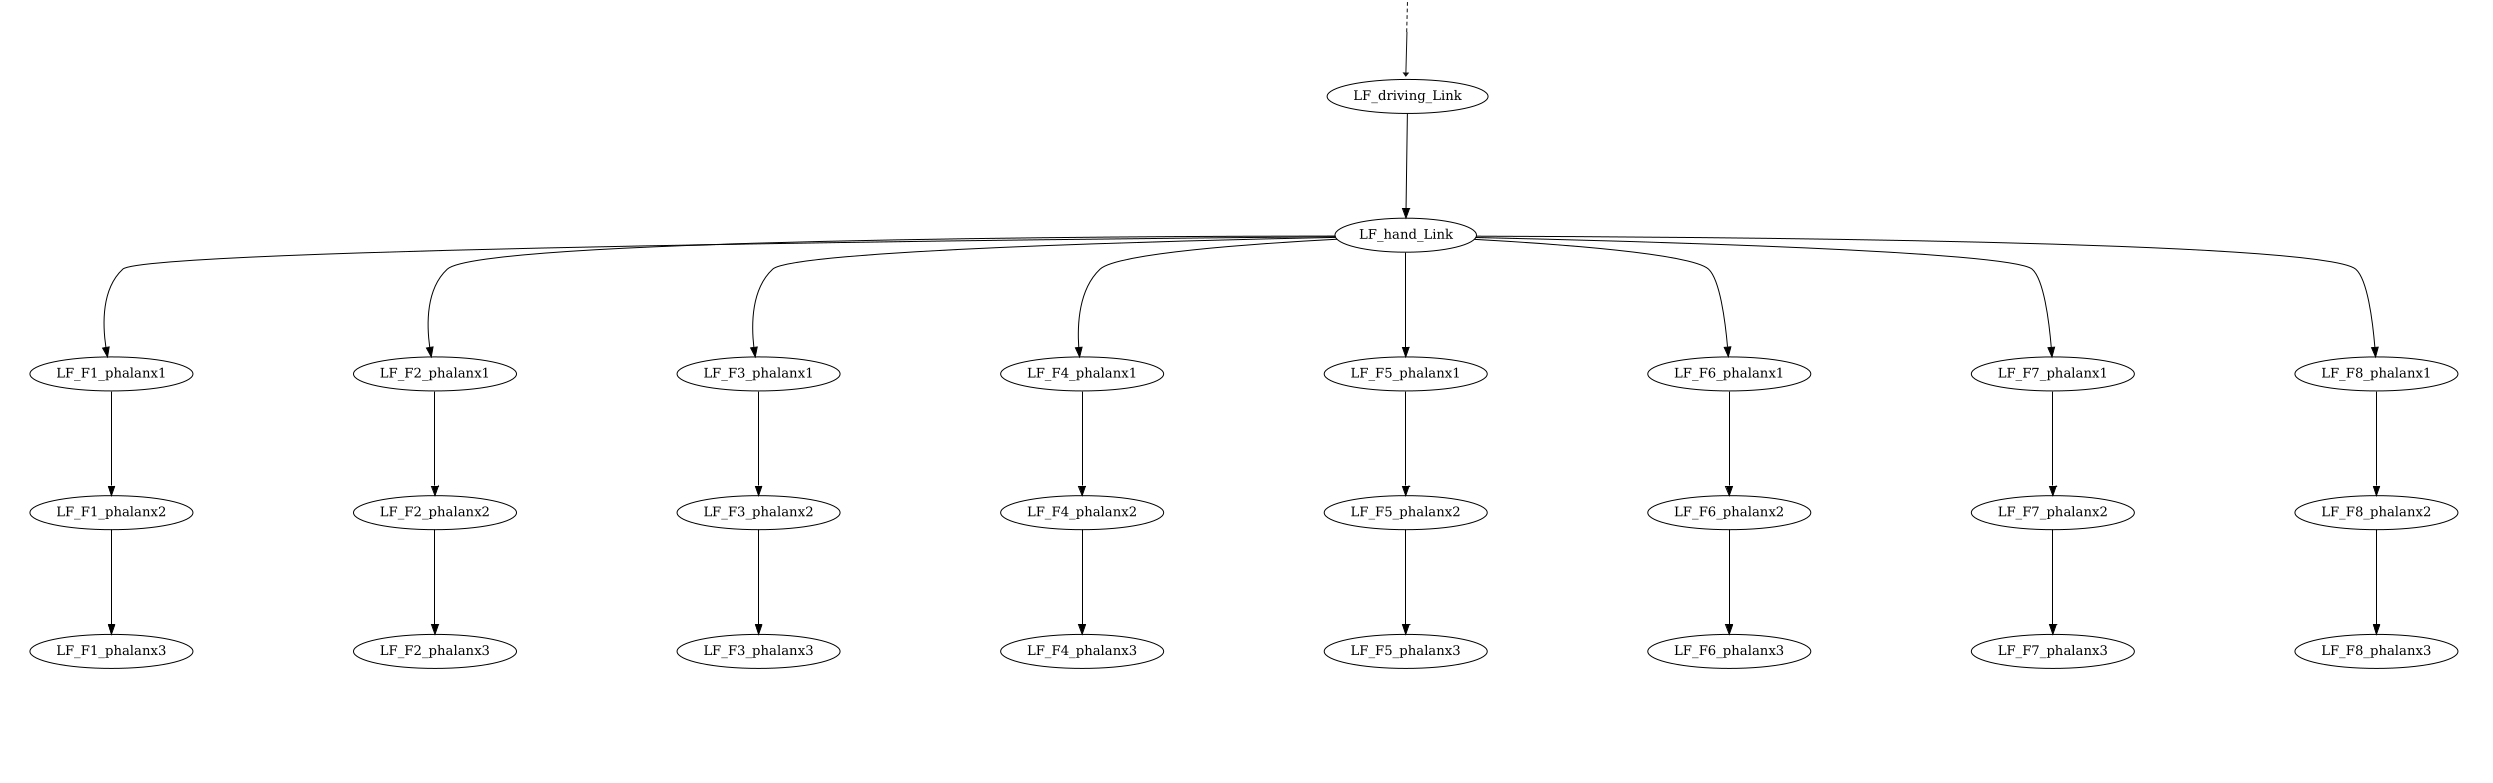
\includegraphics[width=1.0\textwidth]{Images/img_ch4/TFTree_FINGERS.png}
    \caption{Links structure of LF GRIEEL module joints, it is the expansion of LF\_gripper/wheel\_Link of Fig.\ref{fig:TFTree_NOFINGERS}, with a complete links-joints structure of the module, the same holds for LH,RH, and RF.}
    \label{fig:TFTree_FINGERS}
\end{figure}

During the design of GRIEEL, also the mounting mechanism has been developed with the specific purpose of transitioning efficiently between the two locomotion modes and driving the wheels.\\ 
The configuration transition and wheel rotation are achieved with the DOFs previously described, wristH and wristV joints for the first task, while driving joint for the second. Fig.\ref{fig:GRIEEL_GRIPPER_WHEEL} represents the standard configuration in the two modes:
\begin{itemize}
    \setlength\itemsep{-0.5em} 
    \item \textbf{Gripper mode}: $wristH = 0 \;, \; wristV = 0$
    \item \textbf{Wheel mode}: $wristH = \pi \;, \; wristV = \frac{\pi}{2}$
\end{itemize}

The W2G mode transition sequence is represented below in Fig.\ref{fig:GRIEEL_mode_transition}.
\begin{figure}[H]
    \centering
    \subfloat[Wheel mode \\($wristH = \pi, wristV = \pi/2$)\label{fig:W2G_1}]{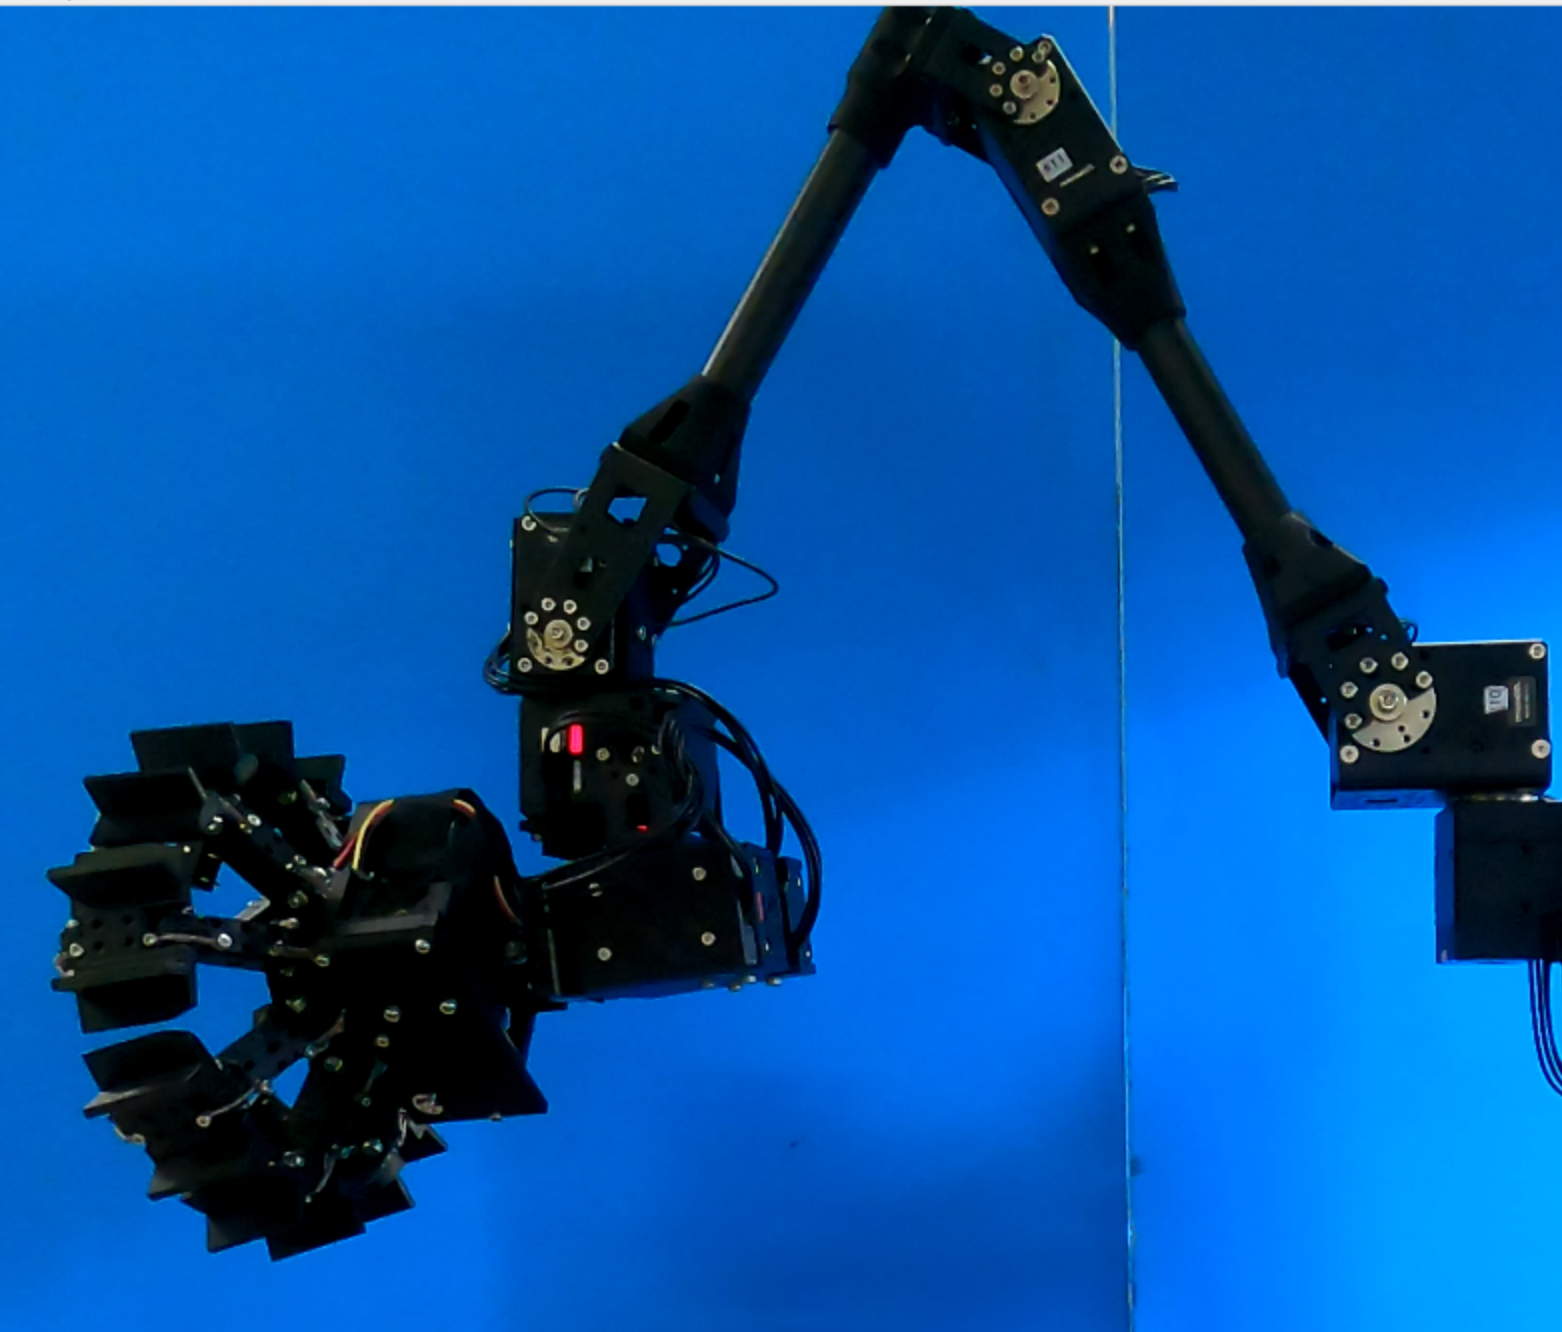
\includegraphics[width=0.3\textwidth]{Images/img_ch4/W2G_1.png}} \quad 
    \subfloat[Start transition of wrist\label{fig:W2G_2}]{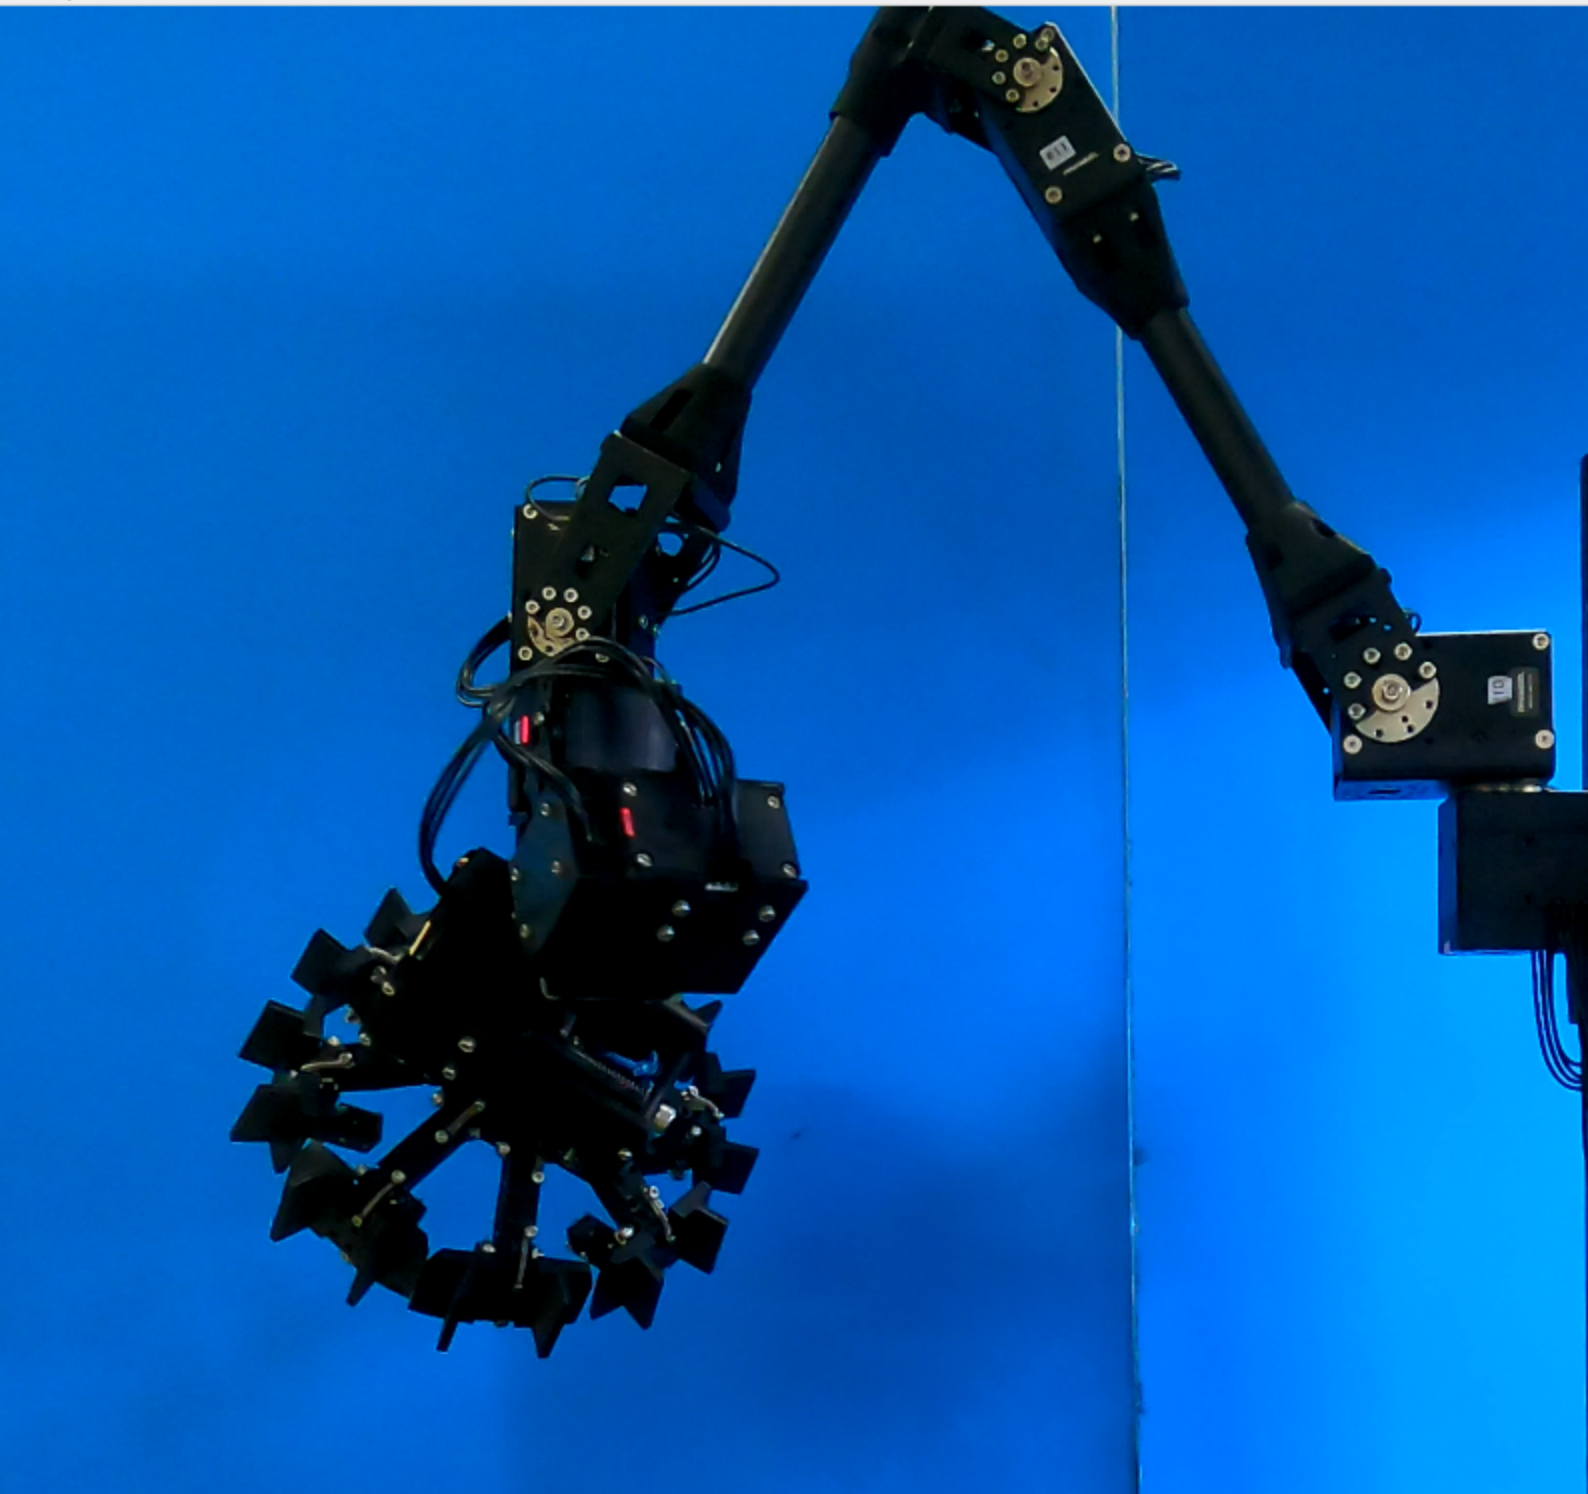
\includegraphics[width=0.3\textwidth]{Images/img_ch4/W2G_2.png}} \quad
    \subfloat[Reached wrist config.\label{fig:W2G_3}]{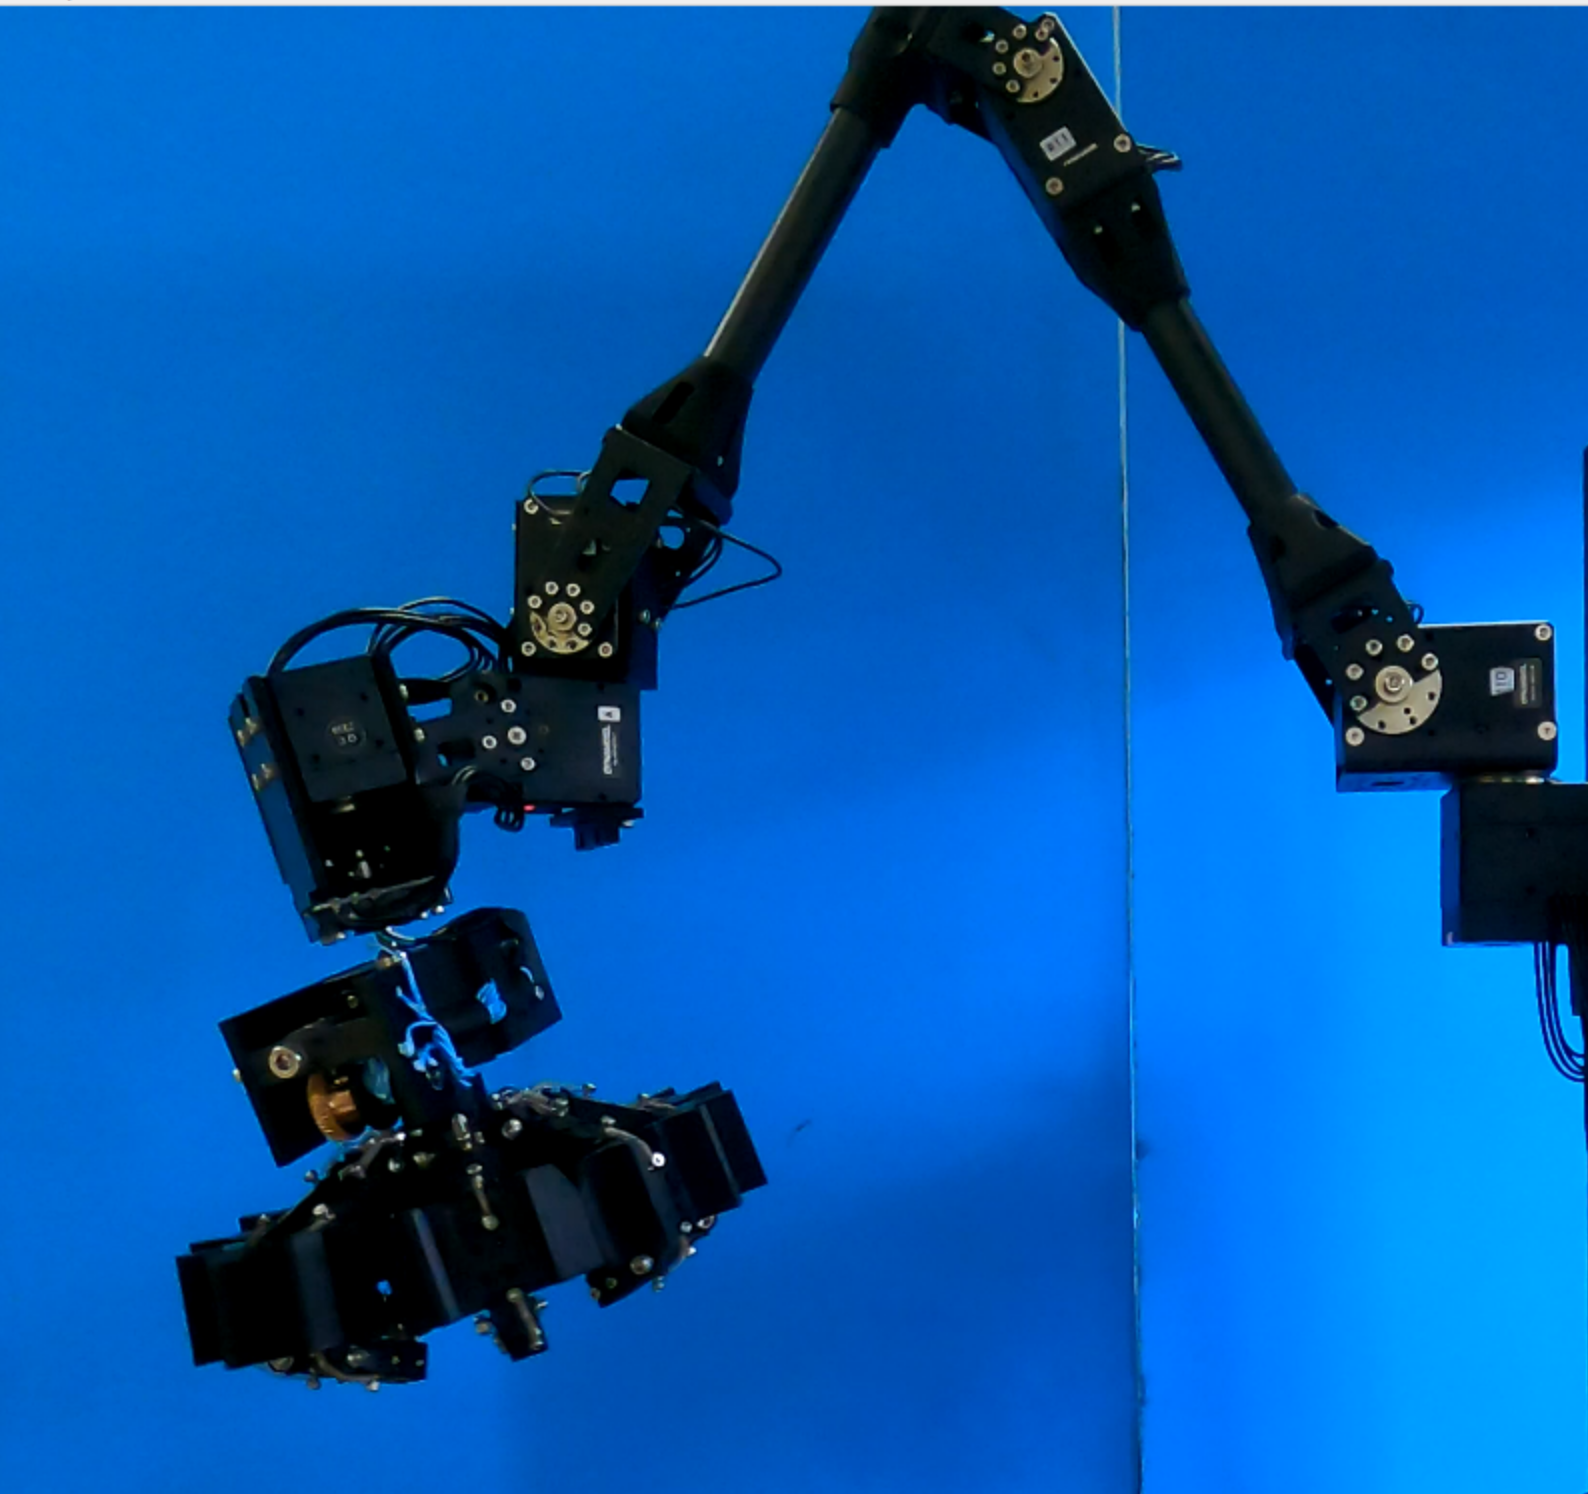
\includegraphics[width=0.3\textwidth]{Images/img_ch4/W2G_3.png}}   \quad
    \\
    \subfloat[Releasing the tethers\label{fig:W2G_4}]{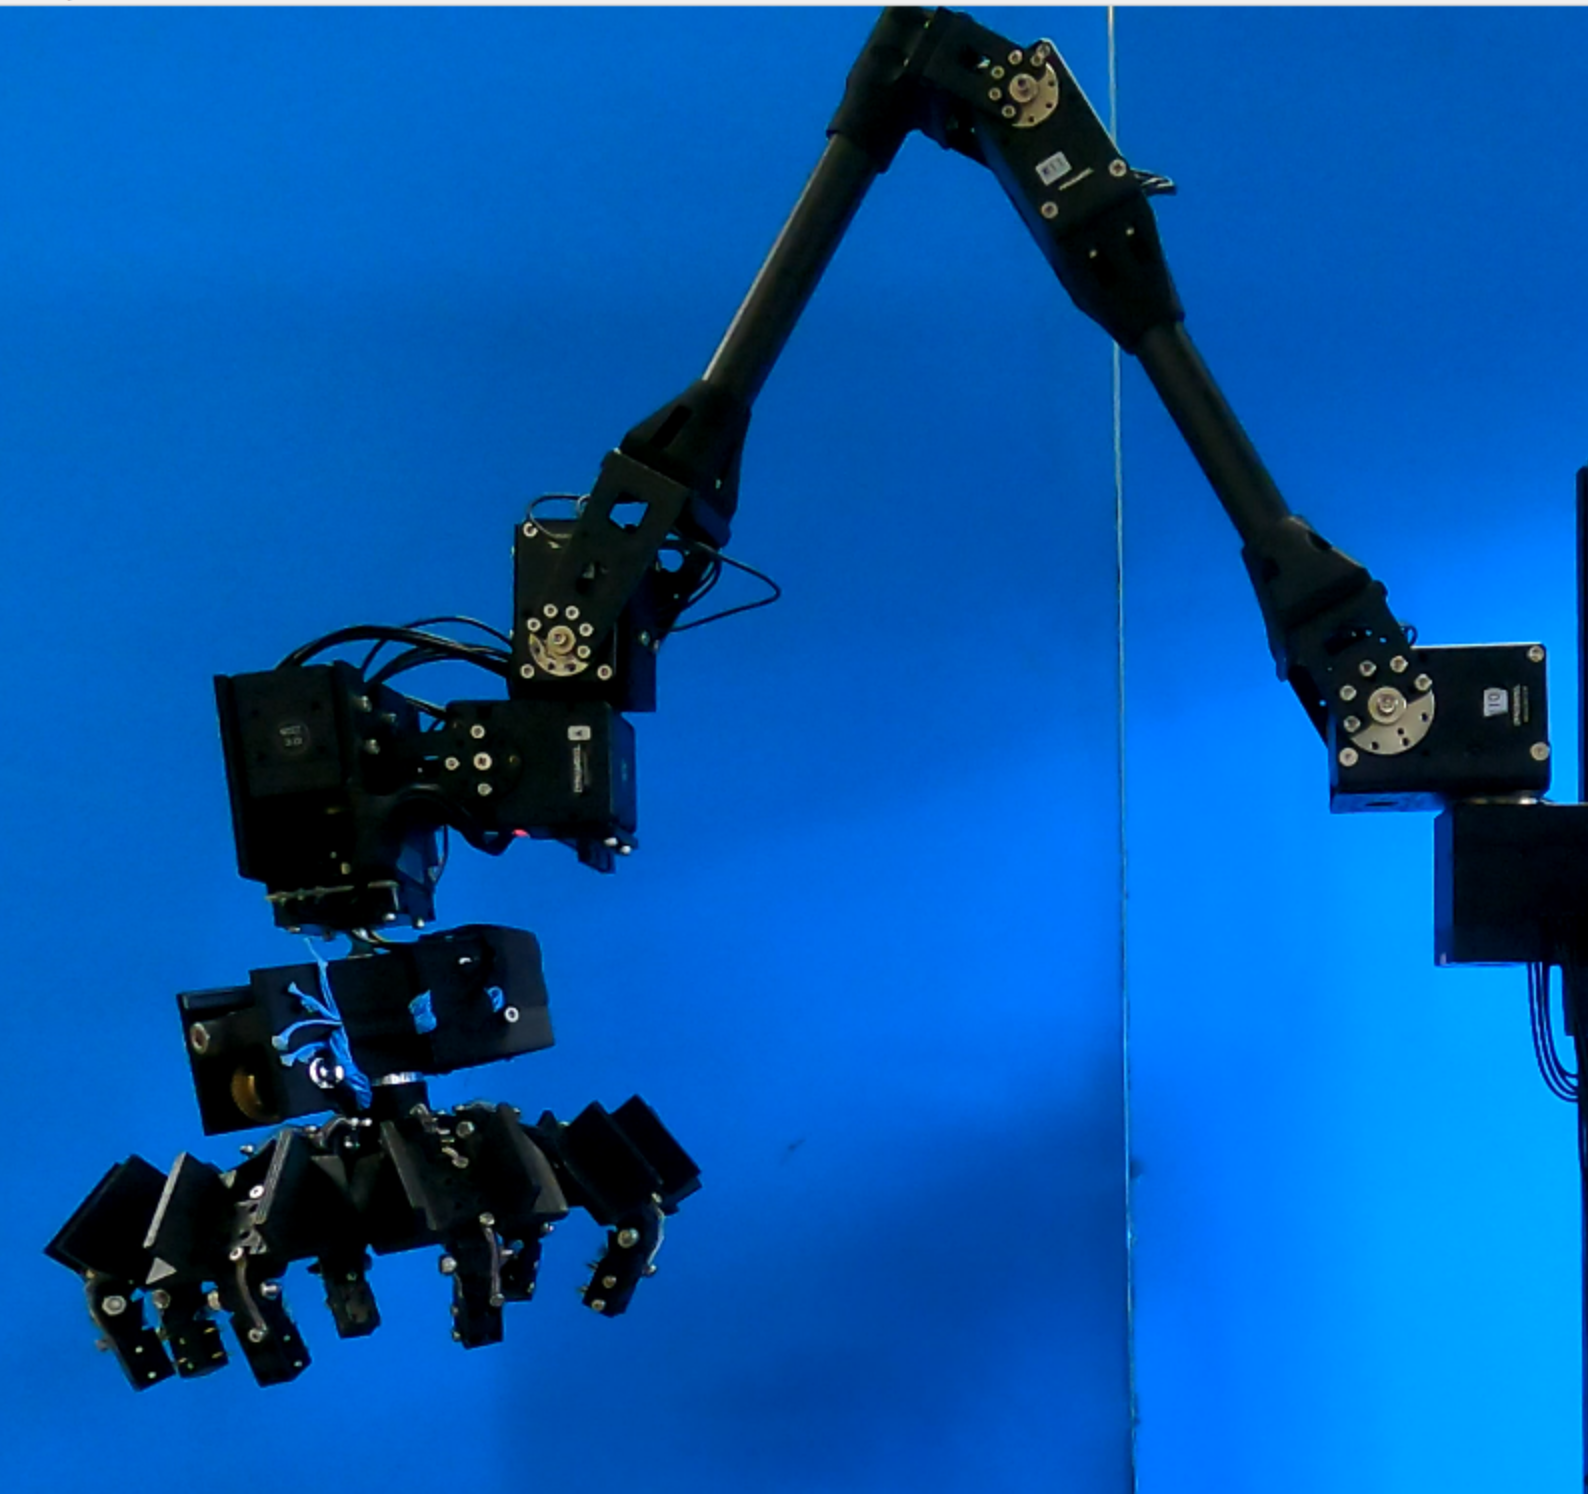
\includegraphics[width=0.3\textwidth]{Images/img_ch4/W2G_4.png}}\quad
    \subfloat[Gripper mode\\($wristH =0, wristV = 0$)\label{fig:W2G_5}]{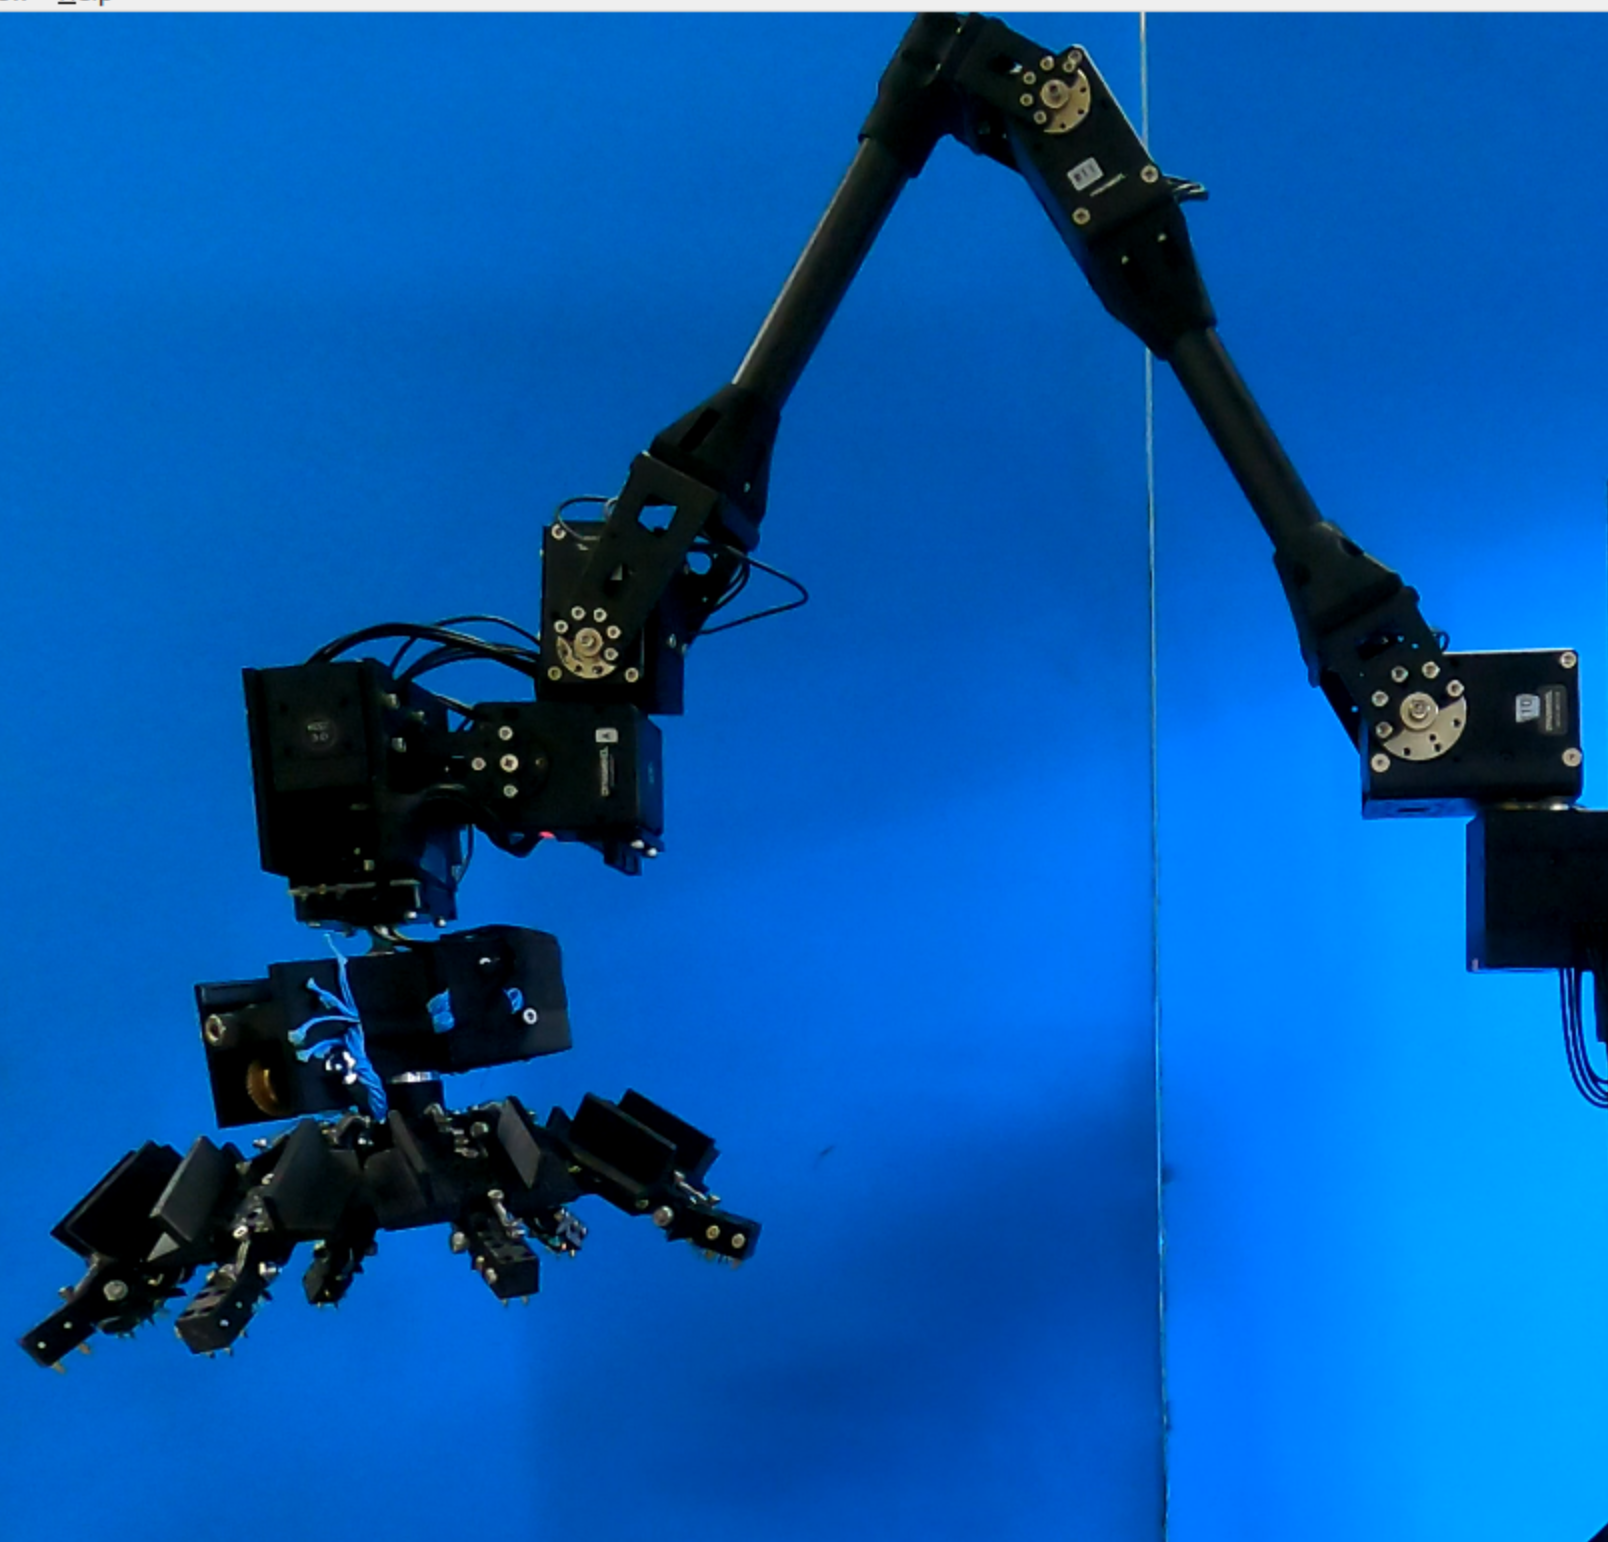
\includegraphics[width=0.3\textwidth]{Images/img_ch4/W2G_5.png}}
    
    \caption[W2G transition sequence]{W2G transition sequence}
    \label{fig:GRIEEL_mode_transition}
\end{figure}

\subsection{Kinematics}
\label{sec:kin}

FK and IK computations, required for motion control of the end-effector, are computed analytically from geometric considerations. The explicit expression is not reported here because not relevant to this research, instead, it is important to clarify the approximation used in those computations. 

As noticed in Chapter \ref{ch:chapter_two}, IK is complex to derive, and the 3 DOFs of GRIEEL (which are not in spherical wrist configuration\cite{Siciliano})  add further complexity. For this reason, the previously developed kinematics computations for LIMBERO's limb are used in the motion controller. This approach is possible if the overall GRIEEL mechanism as a whole is considered as the limb end effector. 

In using this kinematic approximation, the real positioned frame is the one on the link attached to LIMBERO's limb-end, controlled in position and pitch from the previous IK, using the first 4 DOFs. This means that GRIEEL's DOFs are used to control the W2G and G2W transformations and maintained on the desired mode configuration otherwise.  
The details of the implementation of this as part of the kinematics computation in the motion control software are not discussed here.

This choice can be justified by two reasons: 
\begin{enumerate}
   \setlength\itemsep{-0.7em} 
    \item After the first test with the original kinematics, it was noticed that for the tasks involved, there was no need to update the kinematic. 
    limb and base tasks in fact were completed correctly, and mode transition was possible with a decoupled control of wrist joints. 
    \item The design of GRIEEL used in this research is the original prototype, but a new one is under development, as discussed in the last chapter \ref{ch:chapter_nine}. For this reason, rather than defining low-level kinematics computations, more emphasis has been placed on defining high-level algorithms, easy to integrate with the novel system. 
\end{enumerate}

In conclusion, the limb is controlled with the first 4 DOFs in position and pitch angle (which correspond to the sum of $q2+q3+q4$), and mode transition or driving is achieved with a decoupled control of the additional 3 DOFs. However, some tests considering the overall limb structure with its 7 DOFs are conducted with the DH kinematic model defined in MATLAB.

\subsection{Driving, Walking (and Climbing)\\ Locomotion Configurations}
\label{sec:locomotion_configurations}

The potential locomotion capabilities of LIMBERO-GRIEEL are enforced by its redundant limbs, which allow for grasping almost unreachable points during walking or climbing. Even in driving mode, advanced limb configurations could be exploited to achieve better wheeled traversability than conventional rovers. 

the system is not yet ready for such functionality, and now the two main mechanical configurations that have been tested both in simulation and hardware experiments are described. 

\textbf{Walking/Climbing Mode}

The gait scheduler for LIMBERO-GRIEEL is under development, and advanced algorithms for foothold planning will be integrated \cite{LIMBEROTakadaThesis}. 
As discussed, the default walking/climbing configuration uses an insect leg configuration \cite{KentaroUnoPhD}\cite{Todd}, which is represented in Fig.\ref{fig:limbero_walking}.  

\begin{figure}[H]
    \centering
    \subfloat{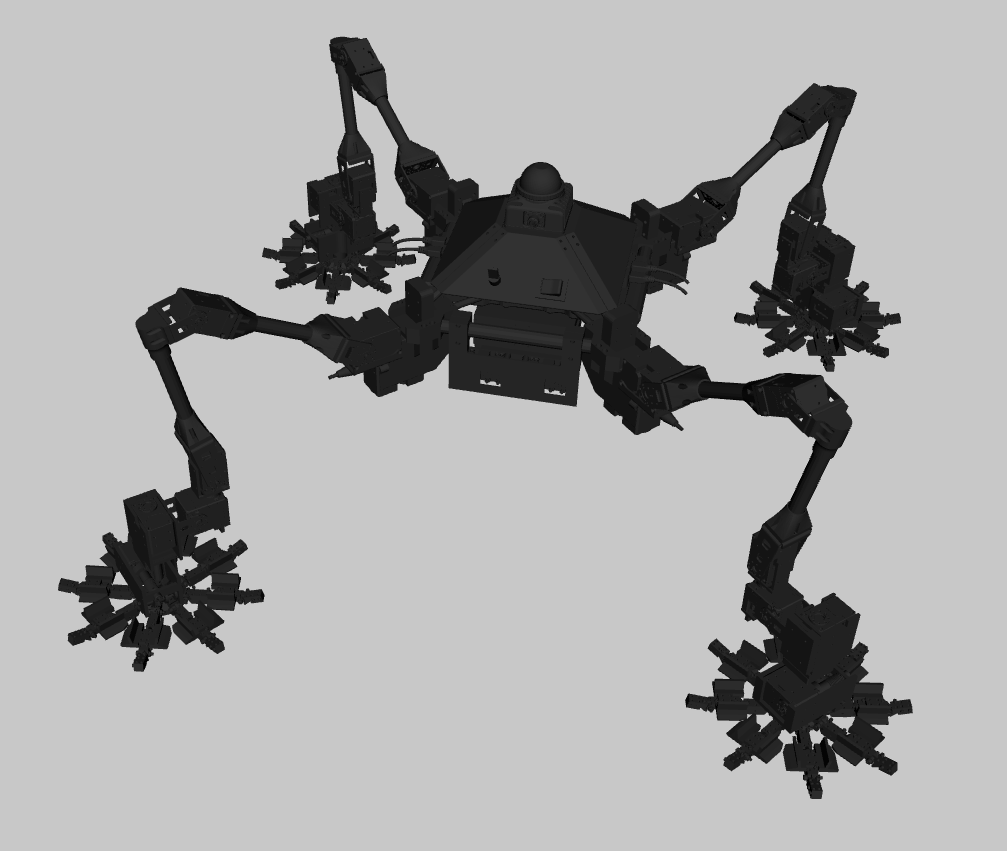
\includegraphics[width=0.45\textwidth]{Images/img_ch4/LIMBERO_GRIEEL_walking.png}}\quad
    \subfloat{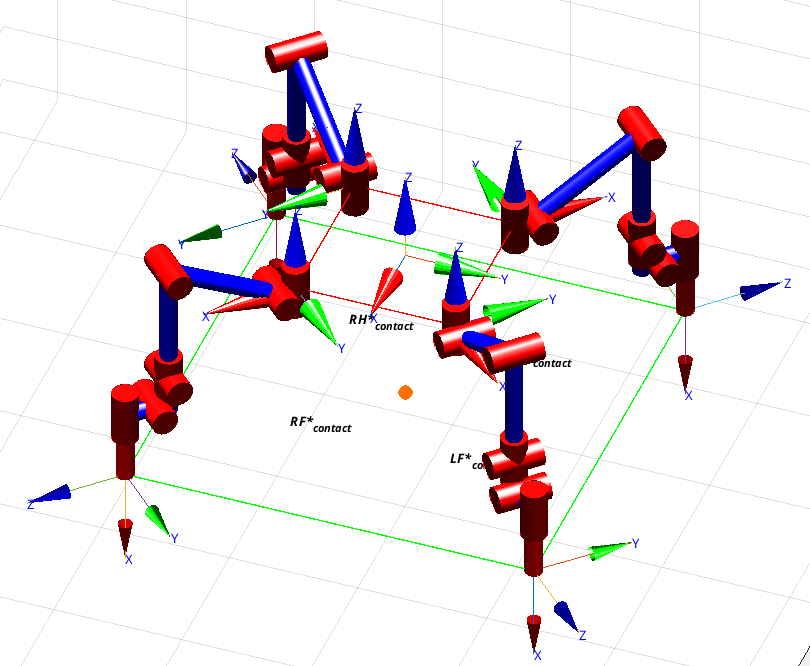
\includegraphics[width=0.45\textwidth]{Images/img_ch4/LIMBERO_GRIEEL_walking_model.png}}
    \caption[LIMBERO-GRIEEL model in wolking/climbing configuration]{LIMBERO-GRIEEL model in wolking/climbing configuration}
    \label{fig:limbero_walking}
\end{figure}

\textbf{Driving Mode}

In principle, $wristH$ joint can be used to perform omnidirectional drive capabilities\cite{Siciliano}. Even if at the current state, driving locomotion has not been designed, wheel rotation commands have been integrated into the limb control software during this research. With this command, it is possible to test the controller's performance when rotating the wheels and perform simple driving tests in simulation. 

To test wheeled locomotion, a simple driving limbs configuration has been considered with wheels facing forward, parallel to the base frame x direction. This configuration is represented in Fig.\ref{fig:limbero_driving} below.
\begin{figure}[H]
    \centering
    \subfloat{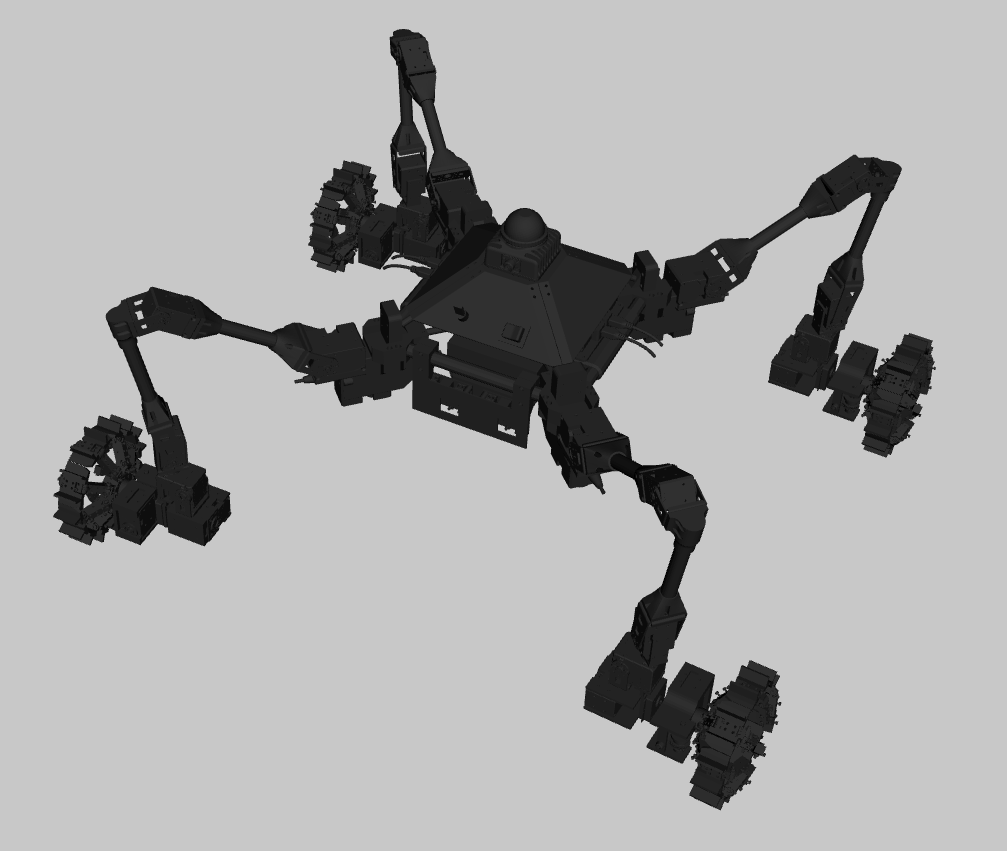
\includegraphics[width=0.45\textwidth]{Images/img_ch4/LIMBERO_GRIEEL_driving.png}}\quad
    \subfloat{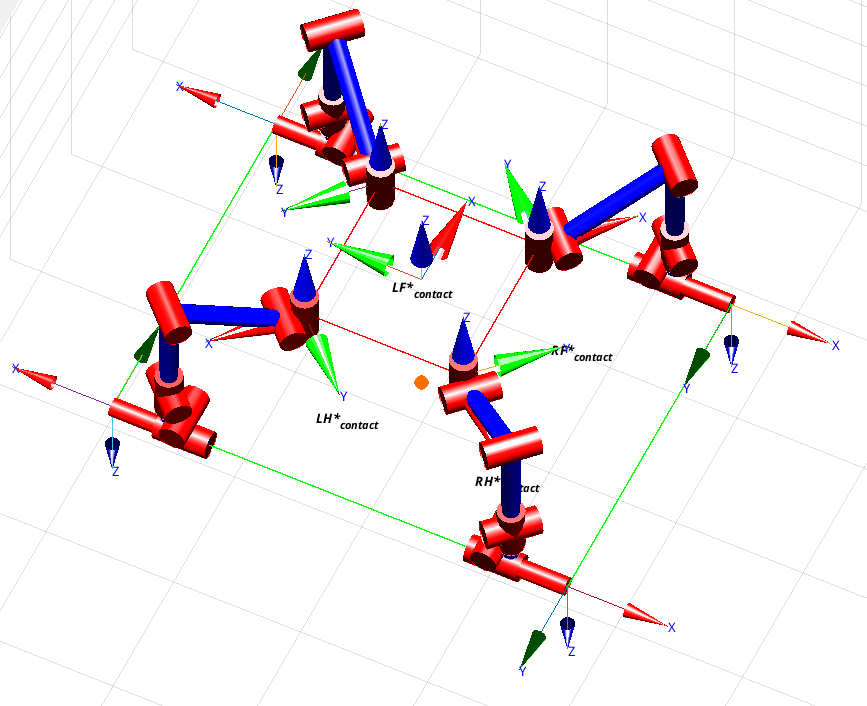
\includegraphics[width=0.45\textwidth]{Images/img_ch4/LIMBERO_GRIEELdriving_model.png}}
    \caption[LIMBERO-GRIEEL model in driving configuration]{LIMBERO-GRIEEL model in driving configuration}
    \label{fig:limbero_driving}
\end{figure}

In this standard driving configuration, it is possible to drive LIMBERO-GRIEEL forward/backward, using the limbs as rigid wheel attachments.

As is evidenced by much research on wheel-on-leg rovers, integrating active limb reconfigurations can equalize traction forces on wheels, ensuring narrow passageways and clamber over obstacles\cite{MAMMOTH}\cite{WheelLeggedStabilityOPT}\cite{WheleedLeggedLUNAR}\cite{WheeledLeggedAMAZONFOREST}. This will be integrated in the final driving controller.

\subsection{Electronics}
\label{sec:electronics}

The main brain of the robot is an NVIDIA Jatson Orin NX, running on board all the software components described in the next autonomously, or remotely operated connecting via SSH.
Several sensors to monitor the robot's state are integrated, Including an RT-USB-9axiIMU2 inertial measurement unit (IMU) and a Livox Mid-360 3D LiDAR \cite{LIMBEROTakadaThesis}.

The feedback of the joint state (fundamental for motion control) is measured by the encoders of the all-in-one servomotors used to control the joint angle, which integrate both incremental encoders and temperature sensors.
These actuators, used to control limb joints and wind the gripper-wheel tethers are DYNAMIXEL servo motors \cite{dynamixel}, all-in-one and smart actuators with many built-in functions, easy to integrate with the software that control the robot.
Tab.\ref{table:DYNAMIXEL} summarizes the servomotor used for each joint  (the tether winding is referred to as locking), with relevant information taken from the data sheet.

\begin{table}[H]
\centering 
    \caption{DYNAMIXEL servo motors of limbs joints}
    \label{table:DYNAMIXEL}
    \begin{tabular}{ c }
    \textbf{Limb Joints Motors}
    \end{tabular}
    \begin{tabular}{| c | c | c | c | c | c | c|}
    \hline
    \rowcolor{bluepoli!40}
%    \rowcolor{bluepoli!40}
     \textbf{Joint} &  DYNAMIXEL & $N_{gear}$ & \textbf{$\tau^*$} $[N m]$ & {$\omega^*$}  $[rad/s]$ & Control Mode \T\B \\
    \hline \hline
    \textbf{B2C} & XM540-W270-R & 272.5 & 3.18 & 3.37  & Position  \T\B\\
    \hline 
    \textbf{C2F} & XM540-W270-R & 272.5 & 3.18 & 3.37 & Position  \T\B\\
    \hline
    \textbf{F2T} & XM430-W350-R & 	353.5  & 1.23 & 3.88 & Position \T\B\\
    \hline
    \textbf{T2E} & XM430-W350-R & 	353.5 & 1,23 & 3.88 & Position \B\\
    \hline
    \textbf{wristH} & 2XL430-W250-T & 257.4 &  0.45 & 4.47 & Position \B\\
    \hline
    \textbf{wristV} & 2XL430-W250-T  & 257.4 &  0.45 & 4.47 & Position \B\\
    \hline
    \textbf{driving} & XM430-W350-R  & 353.5 &  1.23 & 3.88  & Velocity  \B\\
    \hline
    \end{tabular}
    \begin{tabular}{ c }
    \\
    \textbf{Gripper-Wheel Locking Motor}
    \end{tabular}
    \begin{tabular}{| c | c | c | c | c | c | c|}
    \hline
    \rowcolor{bluepoli!40}
    \textbf{Actuator} &  DYNAMIXEL & $N_{gear}$ & \textbf{$\tau^*$} $[N m]$ & {$\omega^*$}  $[rad/s]$ & Control Mode \T\B \\
    \hline\hline
    \textbf{locking} & XL430-W250-T & 258.5 &  0.42 & 4.47 & Velocity \B\\
    \hline
    \end{tabular}
\end{table}

Where $\tau^*$ is the rated torque, estimated as the $ 30\% $ of the stall torque $\tau_{stall}$ as $\tau^* = 0.3\cdot\tau_{stall}$, while $\omega^*$ is the rated speed estimated as $70\%$ the no load speed.
  
\section{Software Description, ROS2 Architecture}
\label{sec:software_ros2}

The control architecture of LIMBERO-GRIEEL is consistent with the multi-layered one described in section \ref{sec:leggedControl}, for this reason, a distributed system where multiple modules communicate in real-time is the obvious choice. The Robot Operating System (ROS2)\cite{ROS1_2009}\cite{ROS2_2022}\cite{ROS2_2023}, with new components written in C++, has been chosen as the software infrastructure for communication and control.
ROS2 uses a Data Distribution Service (DDS) for communication, where computational units (nodes) exchange information through named channels (topics) in a networked structure. But the real advantage of using ROS is that it is \textit{"a set of software libraries and tools for building robot applications. From drivers and state-of-the-art algorithms to powerful developer tools, ROS has the open-source tools you need for your next robotics project."}\cite{ROS2HumbleDocs}. This intrinsic nature allows the development of robotic systems without reinventing the wheels.  

When this thesis research started at the SRL, the software system was prepared for LIMBERO, but not for the overall LIMBERO-GRIEEL limb. For that reason, the first contribution of this work has been a software upgrade, to integrate the new joints and robot model in the ROS2 infrastructure. 

With reference to this multi-layered structure represented in Fig.\ref{fig:LeggedControlScheme}, the motion control of LIMBERO-GRIEEL is based on an IKJC (as discussed in section\ref{sec:leggedControl}), in synthesis, high-level tasks are converted to joint positions through IK computation, then, joint position controllers (JC) move the limbs to the desired configuration.  
The main functionalities that such control software needs are: 
\begin{enumerate}
    \setlength\itemsep{-0.7em} 
    \item Listen and process operator commands (or autonomous planning tasks)
    \item Keep track of the internal state of the robot
    \item Convert the received high-level tasks to limb commands 
    \item Control the limbs 
\end{enumerate}

Autonomous planning requires additional functionalities at a high level (such as path planning) and localization and mapping integration through exteroceptive sensors. Those aspects are not discussed here, since currently autonomy is in development, and the robot is operated from a PC or with a joystick. This research moves in the direction of full autonomy, with the intelligent GRIEEL transition algorithm discussed in the next chapter.   

For the four functionalities listed above, the software needs: teleoperation and Command Line Interface (CLI)(1), robot model representation(2,3),  FK and IK (2,3,4), motor control(4), and support pattern/polygon (SP) estimation(2).

Now the final software infrastructure is briefly discussed in its main components.

First, the model of the robot is represented with the Unified Robotic Descriptive Format (URDF), which is fundamental for controlling both the real system and the simulated one. This is a standard way to represent the robot as a set of links and joints, where each link has its reference frame, and ROS uses TransForm (TF) to update the internal state of the robot, computing homogenous transformation between frames at run time, using joints state.
The tree structure of LIMBERO-GRIEEL represented in Fig.\ref{fig:TFTree_NOFINGERS} and Fig.\ref{fig:TFTree_FINGERS} are derived from two different URDF, and computed directly with ROS2 TF tools. 

The multi-layered structure is represented with a simplified scheme in Fig.\ref{fig:ros2_simple_scheme}, where many of the exchange channels and important feedback have been condensed or neglected for clarity (the complete network visualized from ROS is big and entangled, reporting it here is neither easy nor informative).

Before describing the software components of the ROS-based system, it is important to explain how motion commands are represented. Motion messages are represented by custom \textbf{lbr\_msgs} interface, defining a framework easy to use and understand: 
\begin{itemize}
    \setlength\itemsep{-0.7em} 
    \item \textbf{Limb Motion Task} (LMT):\\ Stores information on limb motion regarding limb ID, duration, and displacement.
    \item \textbf{Base Motion Task} (BMT):\\ Stores information on base motion as duration and displacement.
    \item \textbf{Motion Task} (MT): \\Stores a base or limb motion task with the order of its execution.
    \item \textbf{Motion Package} (MP):\\ Collects an array of motion tasks.
    \item \textbf{Grieel Mode Change} (GMC): \\Stores information on GRIEEL mode transition as limb ID and new mode.
\end{itemize}
The limb ID is an integer number, between 0 and 3 (0 = LF, 1 = LH, 2 = RH, 3 = RF). 

Furthermore, two types of joint controllers have been tested in simulation, the first is a joint trajectory controller (JTC), based on the ros2\_control framework (which is a collection of ROS2 packages and functionalities to control robots). 
The second is a custom controller based on the IJC explained in \ref{sec:IndipendentJointControl}. Tuning in the simulation was then adjusted for DYNAMIXEL servos. 
Additional details on how these controllers are structured and their tuning approach are addressed in chapter \ref{ch:chapter_six}.

The infrastructure is implemented with the following components (“lbr” is an abbreviation for "limbero"), with functionalities of control, state estimation, and motion planning: 
\begin{itemize}
\item \textbf{lbr\_command\_interface} (CI):\\ 
    It processes the operator's input via keyboard or joypad, converting commands to motion tasks for the HLC or LLC.
\item \textbf{lbr\_sim}: \\
    It organized feedback and control signals from different limbs in unique data structures. 
    \begin{itemize}
    \setlength\itemsep{-0.7em} 
    \item[-] During simulation, it maps each limb state (contact and configuration) to a whole joint state, for easier management of it.
    \item[-] During real robot control, it collects into a single data structure the overall motors encoder state. \item[-] After storing the desired joint states from LC, it is responsible for communicating it to the JTC node.
    \end{itemize}
\item \textbf{lbr\_state\_estimator} (SE): \\
Based on the overall joint state (received from lbr\_sim), it has an estimation and debugging visualization purpose. 
    \begin{itemize}
        \setlength\itemsep{-0.7em} 
        \item[-] Publishes each limb EE motion command as marker information for Rviz2, a visualization tool used with ROS2.
        \item [-] Estimate the current state of the robot, such as position, posture, and contact state, based on sensor data.
        \item [-] Limb FK is used to estimate limb-tip 
        position.
        \item [-] Estimate support pattern from contact state and limb-tip position
    \end{itemize}
\item \textbf{lbr\_high\_level\_controller} (HLC):
\begin{itemize}
        \setlength\itemsep{-0.7em} 
        \item[-] Maps operator high level command tasks to LLC messages in terms of simple BMT, LMT, GMC, or complete MP. Examples of high level tasks are gait generation and the grieel transition algorithm explained in chapter \ref{ch:chapter_five}.
        \item [-] Responsible for other high-level functionalities, like checking static stability 
\end{itemize}
\item \textbf{lbr\_low\_level\_controller} (LLC): \\
map LLC tasks command to LC commands, as end effector position of each limb. So it stays in between HLC and LC to coordinate the limbs. 
    \begin{itemize}
    \setlength\itemsep{-0.7em} 
        \item [-] Received a BMT in terms of position and orientation, it is converted to the corresponding EE position, using geometrical computation, 
        \item [-] Received a LMT, it creates the EE sequence of positions. This end-effector trajectory is properly fitted using the initial pose, final, and middle pose (if defined), using a 7-order polynomial trajectory.
    \end{itemize}  
\item \textbf{lbr\_limb\_controller} (LC): \\
LC with LF, LH, RH, and RF namespace are initialized (four LC run simultaneously).  
It is the Middle-level part of the controller structure before the joint controllers and hardware actuation.
    \begin{itemize}
    \setlength\itemsep{-0.7em} 
        \item [-] Each LC controller, receives the EE trajectory step by step and uses IK to map that into the required joint states, needed for checking feasibility and actuating the motors. 
        \item [-] Each LC, uses FK to update at runtime the current EE pose, used to track the state of the task.
        \item [-] Each LC controller converts the corresponding Grieel commands received from LLC into grieel joints, such as mode transition and driving.   
    \end{itemize} 
\item \textbf{lbr\_indipendent\_joint\_controller} (IJC): \\
Currently used only in simulation as an alternative to the ros2\_control JTC.
IJC with LF, LH, RH, and RF namespace are initialized (four IJC run simultaneously). 
Implements the independent joint control decoupled PPI closed-loop control of limbs' joints.
Received the equivalent limb desired joint states and feedback, it processes that information and computes the control law.  
\item \textbf{joint\_trajectory\_controller} (JTC): \\
Currently used only in simulation, the hardware interface to connect it with DYNAMIXEL motors is under development.
It is taken from the ros2\_control framework and implements independent joint control based on closed-loop PID controllers.
Received all limb joints' desired joint trajectory, it processes that information and computes the control signal.  
\item \textbf{lbr\_dynamixel\_controller} (DYC): \\
DYC with LF, LH, RH, and RF namespace are initialized (four DYC run simultaneously).  
In principle, commands computed by JTC of ros2\_control can be mapped directly to the motors, but this requires the definition of a hardware interface. At the current state of the software, motor commands are sent by this additional node, responsible for writing each LC joint state to the correct port where the motor is attached, and reading the encoder state. 
This corresponds to the lowest level of the multi-layer infrastructure. 
\end{itemize}

\begin{figure}[H]
    \centering
    \hspace{-2cm}
    \includegraphics[width=1.1\textwidth]{Images/img_ch4/ros2_simple_scheme.pdf}
    \caption{Simplified ROS architecture}
    \label{fig:ros2_simple_scheme}
\end{figure}


\section{Simulation}
\label{sec:simulation_description}

Simulation is one of the first steps of any robotic system development, providing a virtual environment to test the system without damaging the real hardware \cite{RobotSimulation}\cite{RobotSimulation2}. 
The term \textit{sim to real reliability} is defined as a measure of how much the simulation environment is physically consistent with reality.
If the simulator has a satisfactory sim-to-real, it can be used for: 
\begin{itemize}
    \setlength\itemsep{-0.7em} 
    \item Prototyping the mechanical system without creating the real system, reducing cost. 
    \item Test the software infrastructure without risking damaging the robot.
    \item Test new complex algorithms in a simulated world, hard to reproduce in a real experiment. Such as navigation and mapping in hazardous or unreachable environments.  
    \item Train Robotics reinforcement learning models \cite{RL_overview}\cite{RobotSimulationRL}. 
\end{itemize}

Some of the characteristics that influence the choice of the "best" simulator are: the target environment (ground, underwater, sky), the robot's mechanical characteristics (how important is flexibility), and the target task (motion control, perception, navigation, human-robot collaboration) \cite{RobotSimulation1}.

For this research, two main simulation environments have been used, depending on the testing objective.  Gazebo, which is easy to integrate with ROS and has an integrated physics engine, has been used to test the robot's behavior during motion control. MATLAB-Simulink to tune joints' controllers and improve performances.

\subsection{Gazebo Simulation}
\label{sec:gazebo}

Gazebo is a "set of open source development libraries encapsulating all the essentials, such as common math data types, logging, 3D mesh management, and asynchronous message passing"\cite{gazebo}.

The first step to set up this simulation environment is the definition of the robot.
The robot model is represented with the URDF convention, taking care of defining realistic inertia parameters (CoM, Inertial tensor, masses) and dissipative force in the joints as in contact interactions, such as friction and dumping.
Furthermore, sensors or additional interaction forces can be integrated using plugins. 

For LIMBERO-Grieel simulation, the basic URDF with links, joints, collisions, and inertia is derived from the SolidWorks CAD, and dumping and friction have been derived with an iterative tuning procedure.

The world model is also based on an XML format as the URDF, the SDF(Simulation Description Format), where world elements visuals, collisions, and interaction characteristics are defined, together with additional information such as gravity and physics engine.   

With its open source nature, Gazebo gets continuously updated, not only in terms of bugs and functionalities but also in its infrastructure (as happened for ROS in the transition from ROS1 to ROS2).
For that reason, during this research, two versions of gazebo have been used, with a different joint control approach.
An older version (classic) has been used, with the URDF considering a single Grieel/Wheel link as in Fig.\ref{fig:TFTree_NOFINGERS}, and the JTC based on ros2\_control. 
A newer version, sim (Harmonic) has been used with the complete model integrating actuated Grieel fingers' joints(see Fig.\ref{fig:TFTree_FINGERS}), enabling mode transition during simulation. In Harmonic, the custom IJC to control joints has been implemented, and a ros2\_control gripper controller has been used to control Grieel G2W and W2G transformation. 
The newer gazebo distribution proves to be more stable in handling contact interactions and physics consistency, while in the older, unrealistic behaviors often occur, and tuning the simulation parameters has been harder.

Below some screenshots taken from the two simulators are reported (Classic in Fig.\ref{fig:sim_classic}, Harmonic in Fig.\ref{fig:sim_harmonic}).  

\begin{figure}[H]
    \centering
    \subfloat[Gripper mode \label{fig:sim_classic_a}]{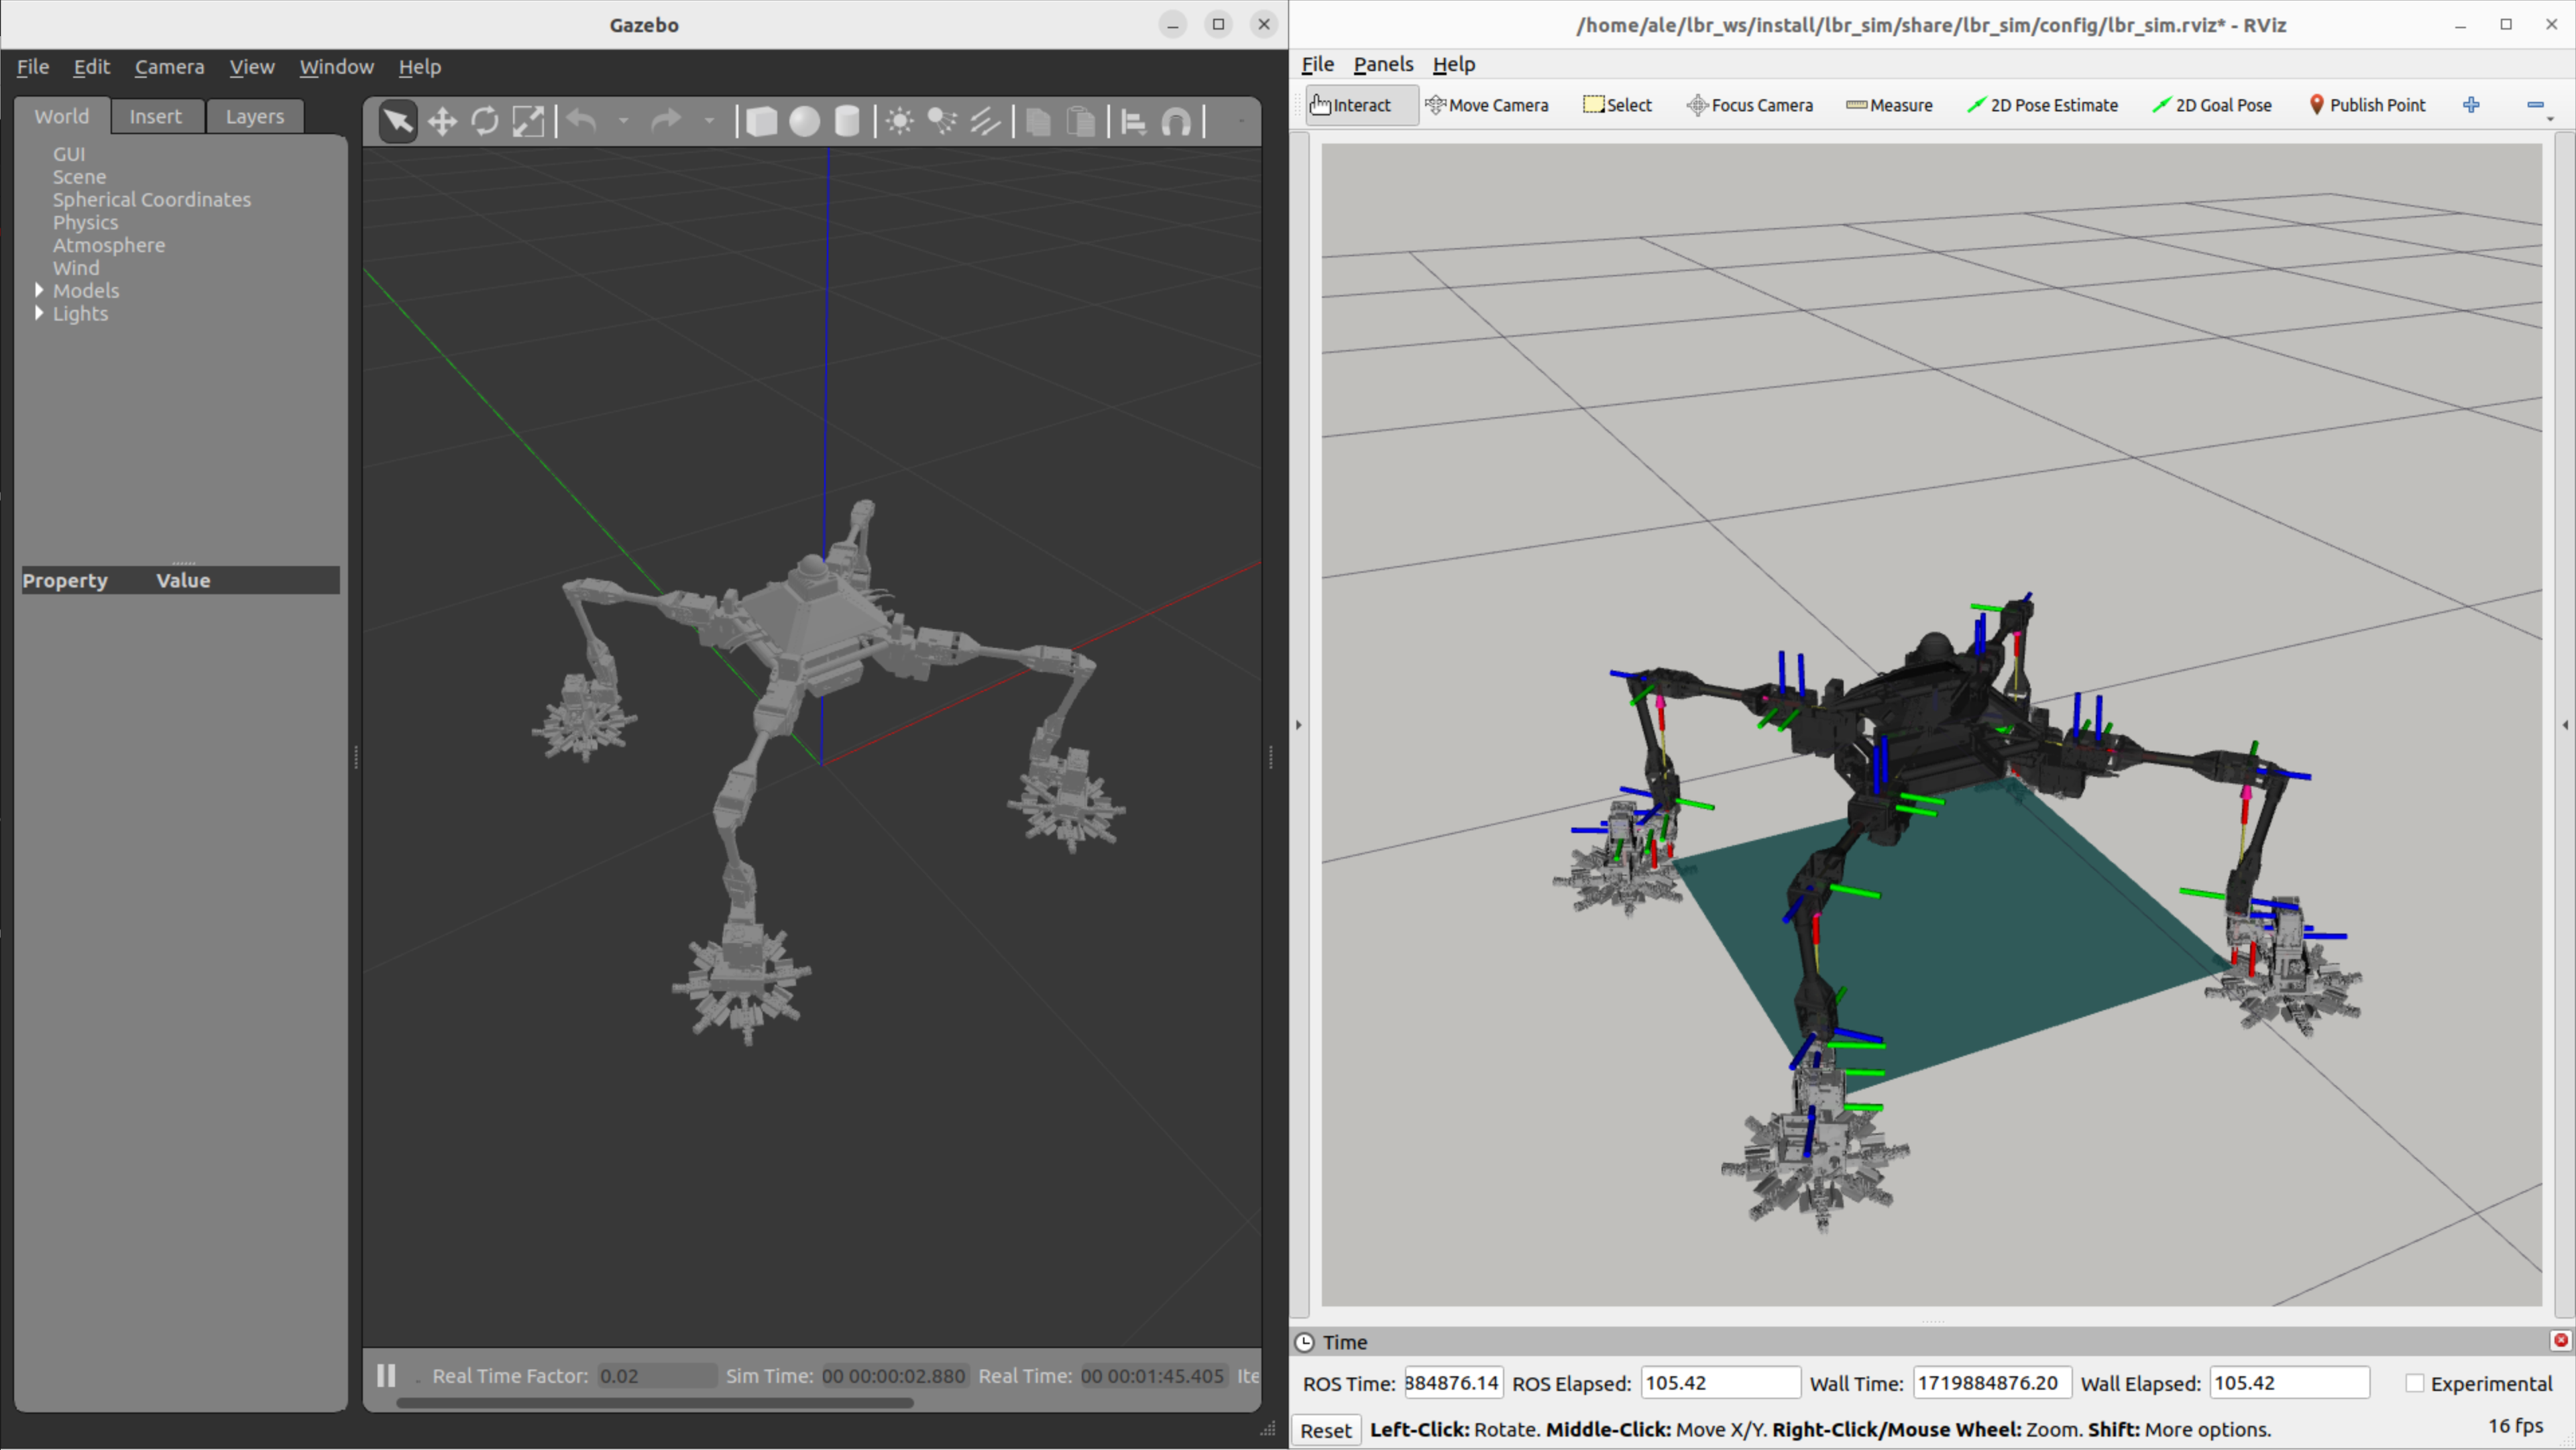
\includegraphics[width=0.4\textwidth]{Images/img_ch4/Classic_Gripper.png}}\quad
    \subfloat[Wheel mode\label{fig:sim_classic_b}]{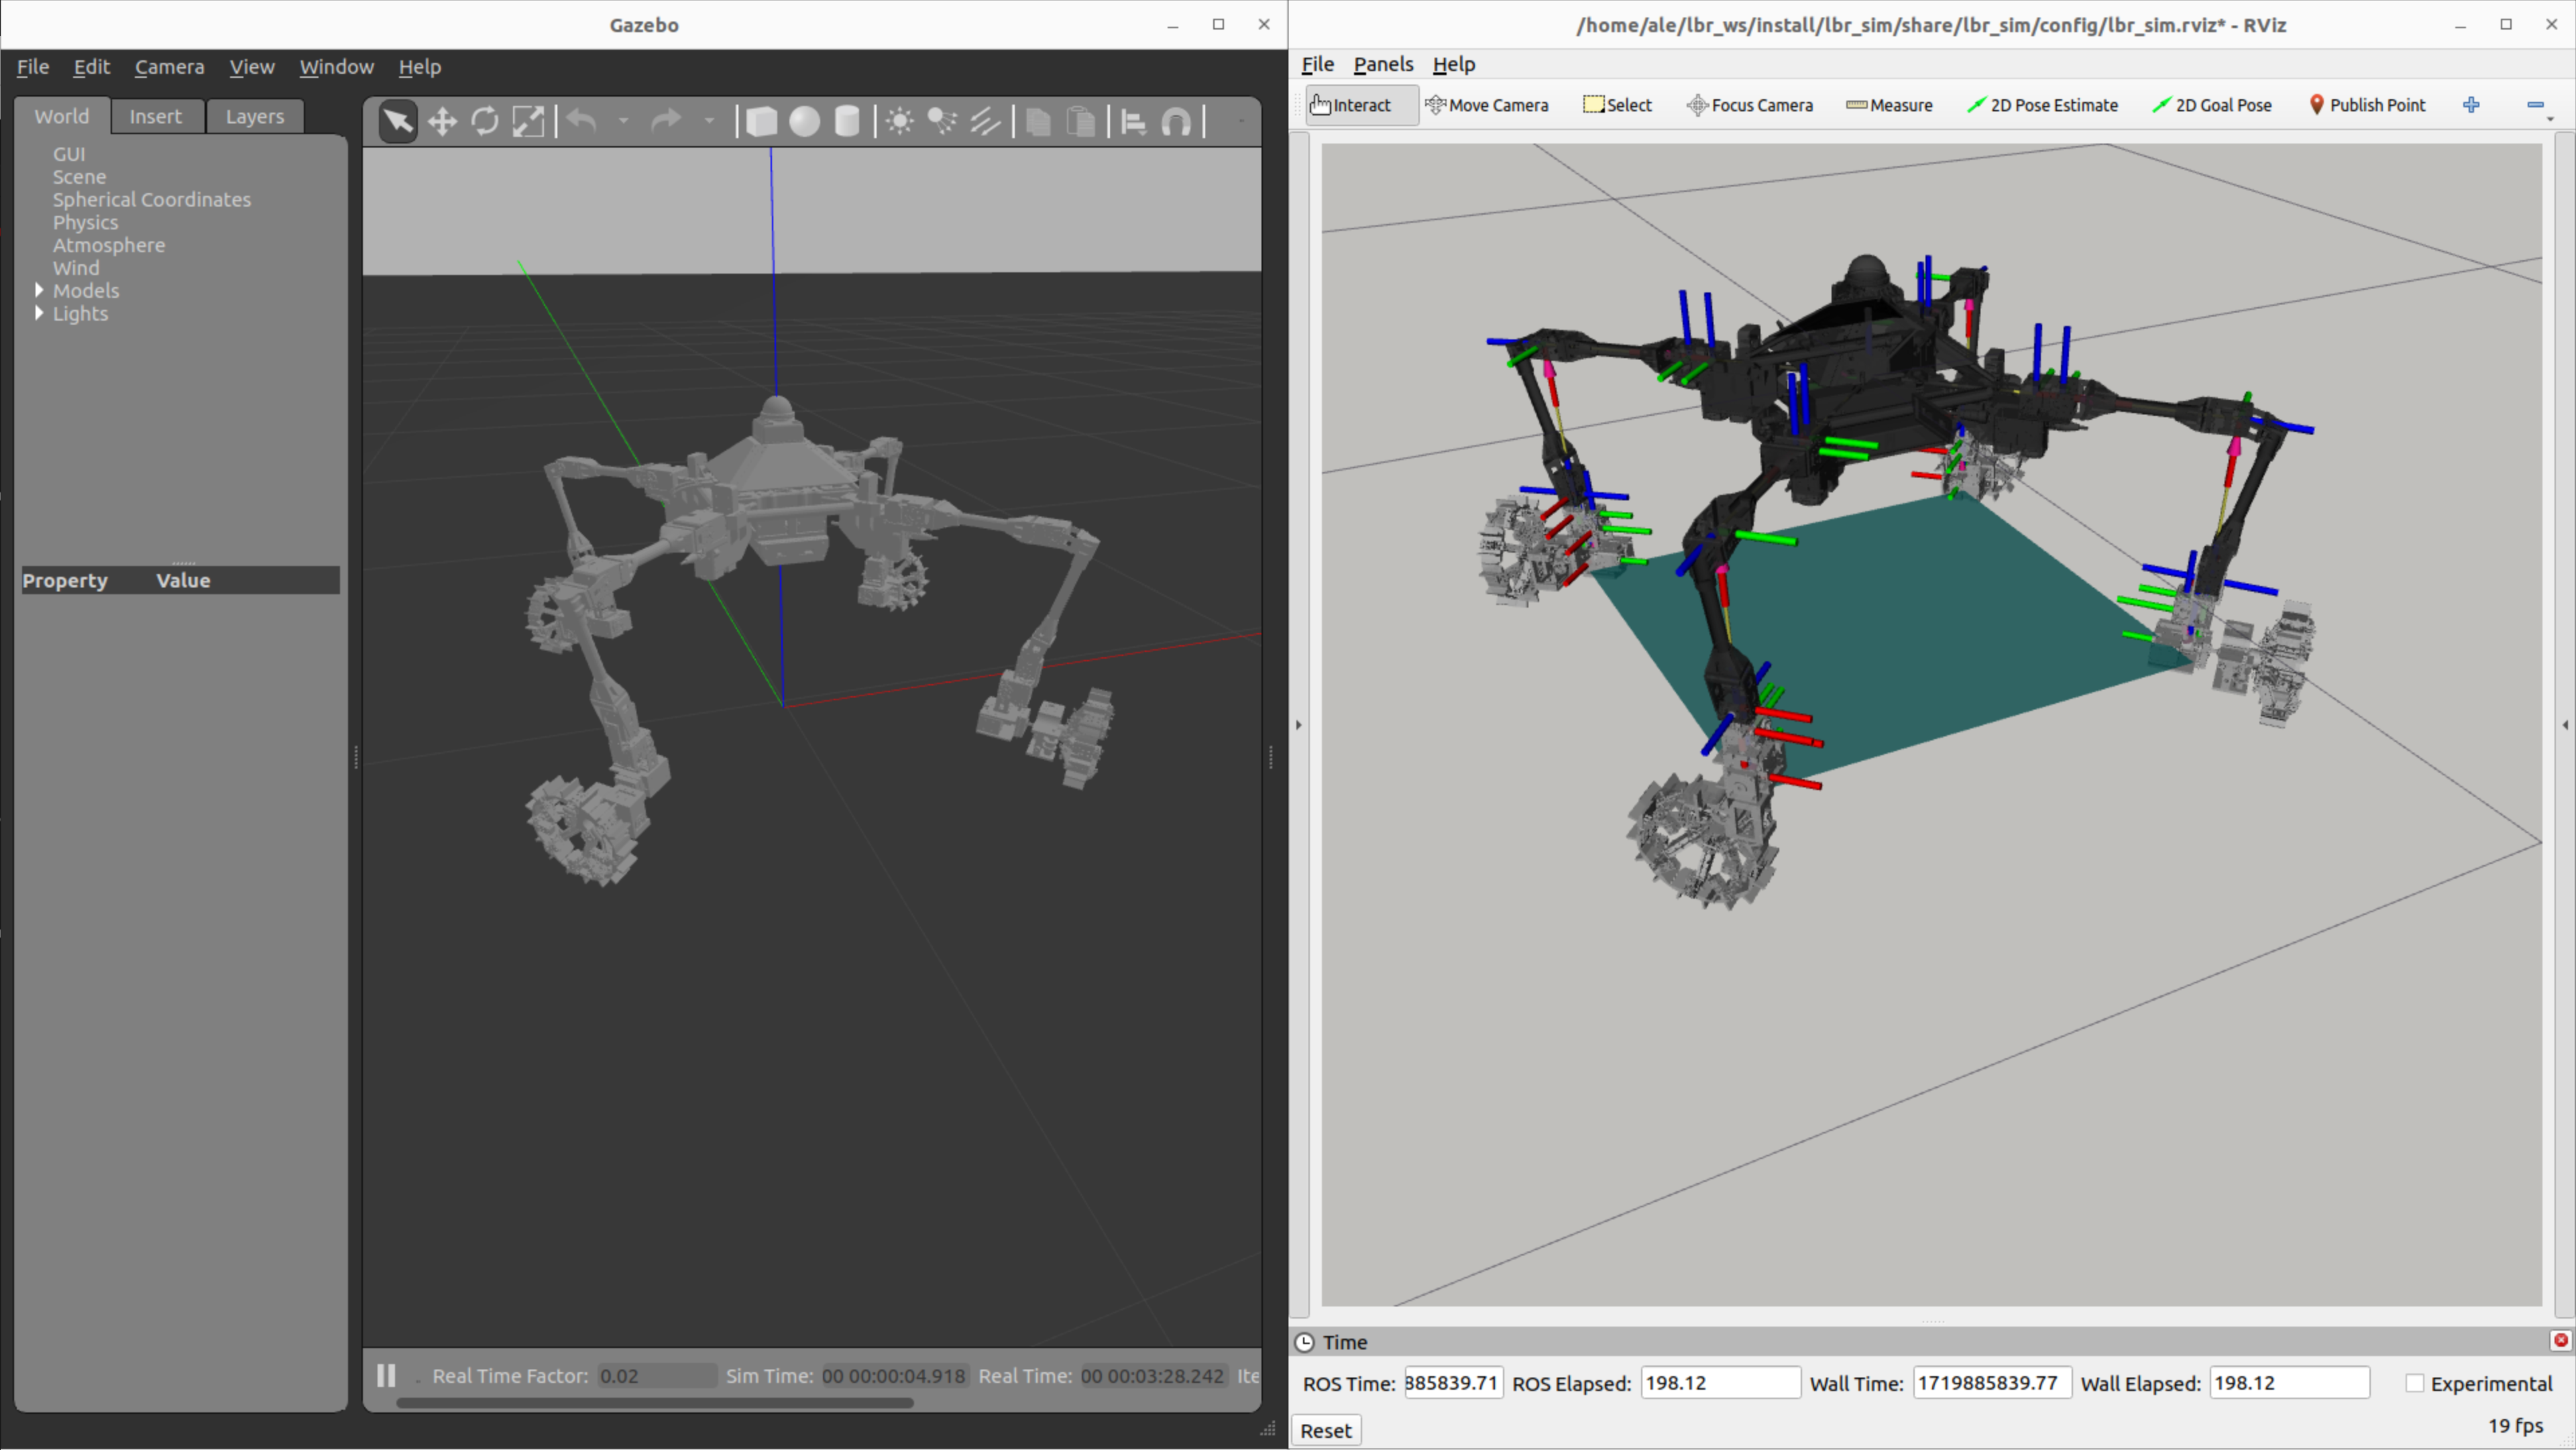
\includegraphics[width=0.4\textwidth]{Images/img_ch4/Classic_Wheel.png}}\\
    \subfloat[Mars environment\label{fig:sim_classic_c}]{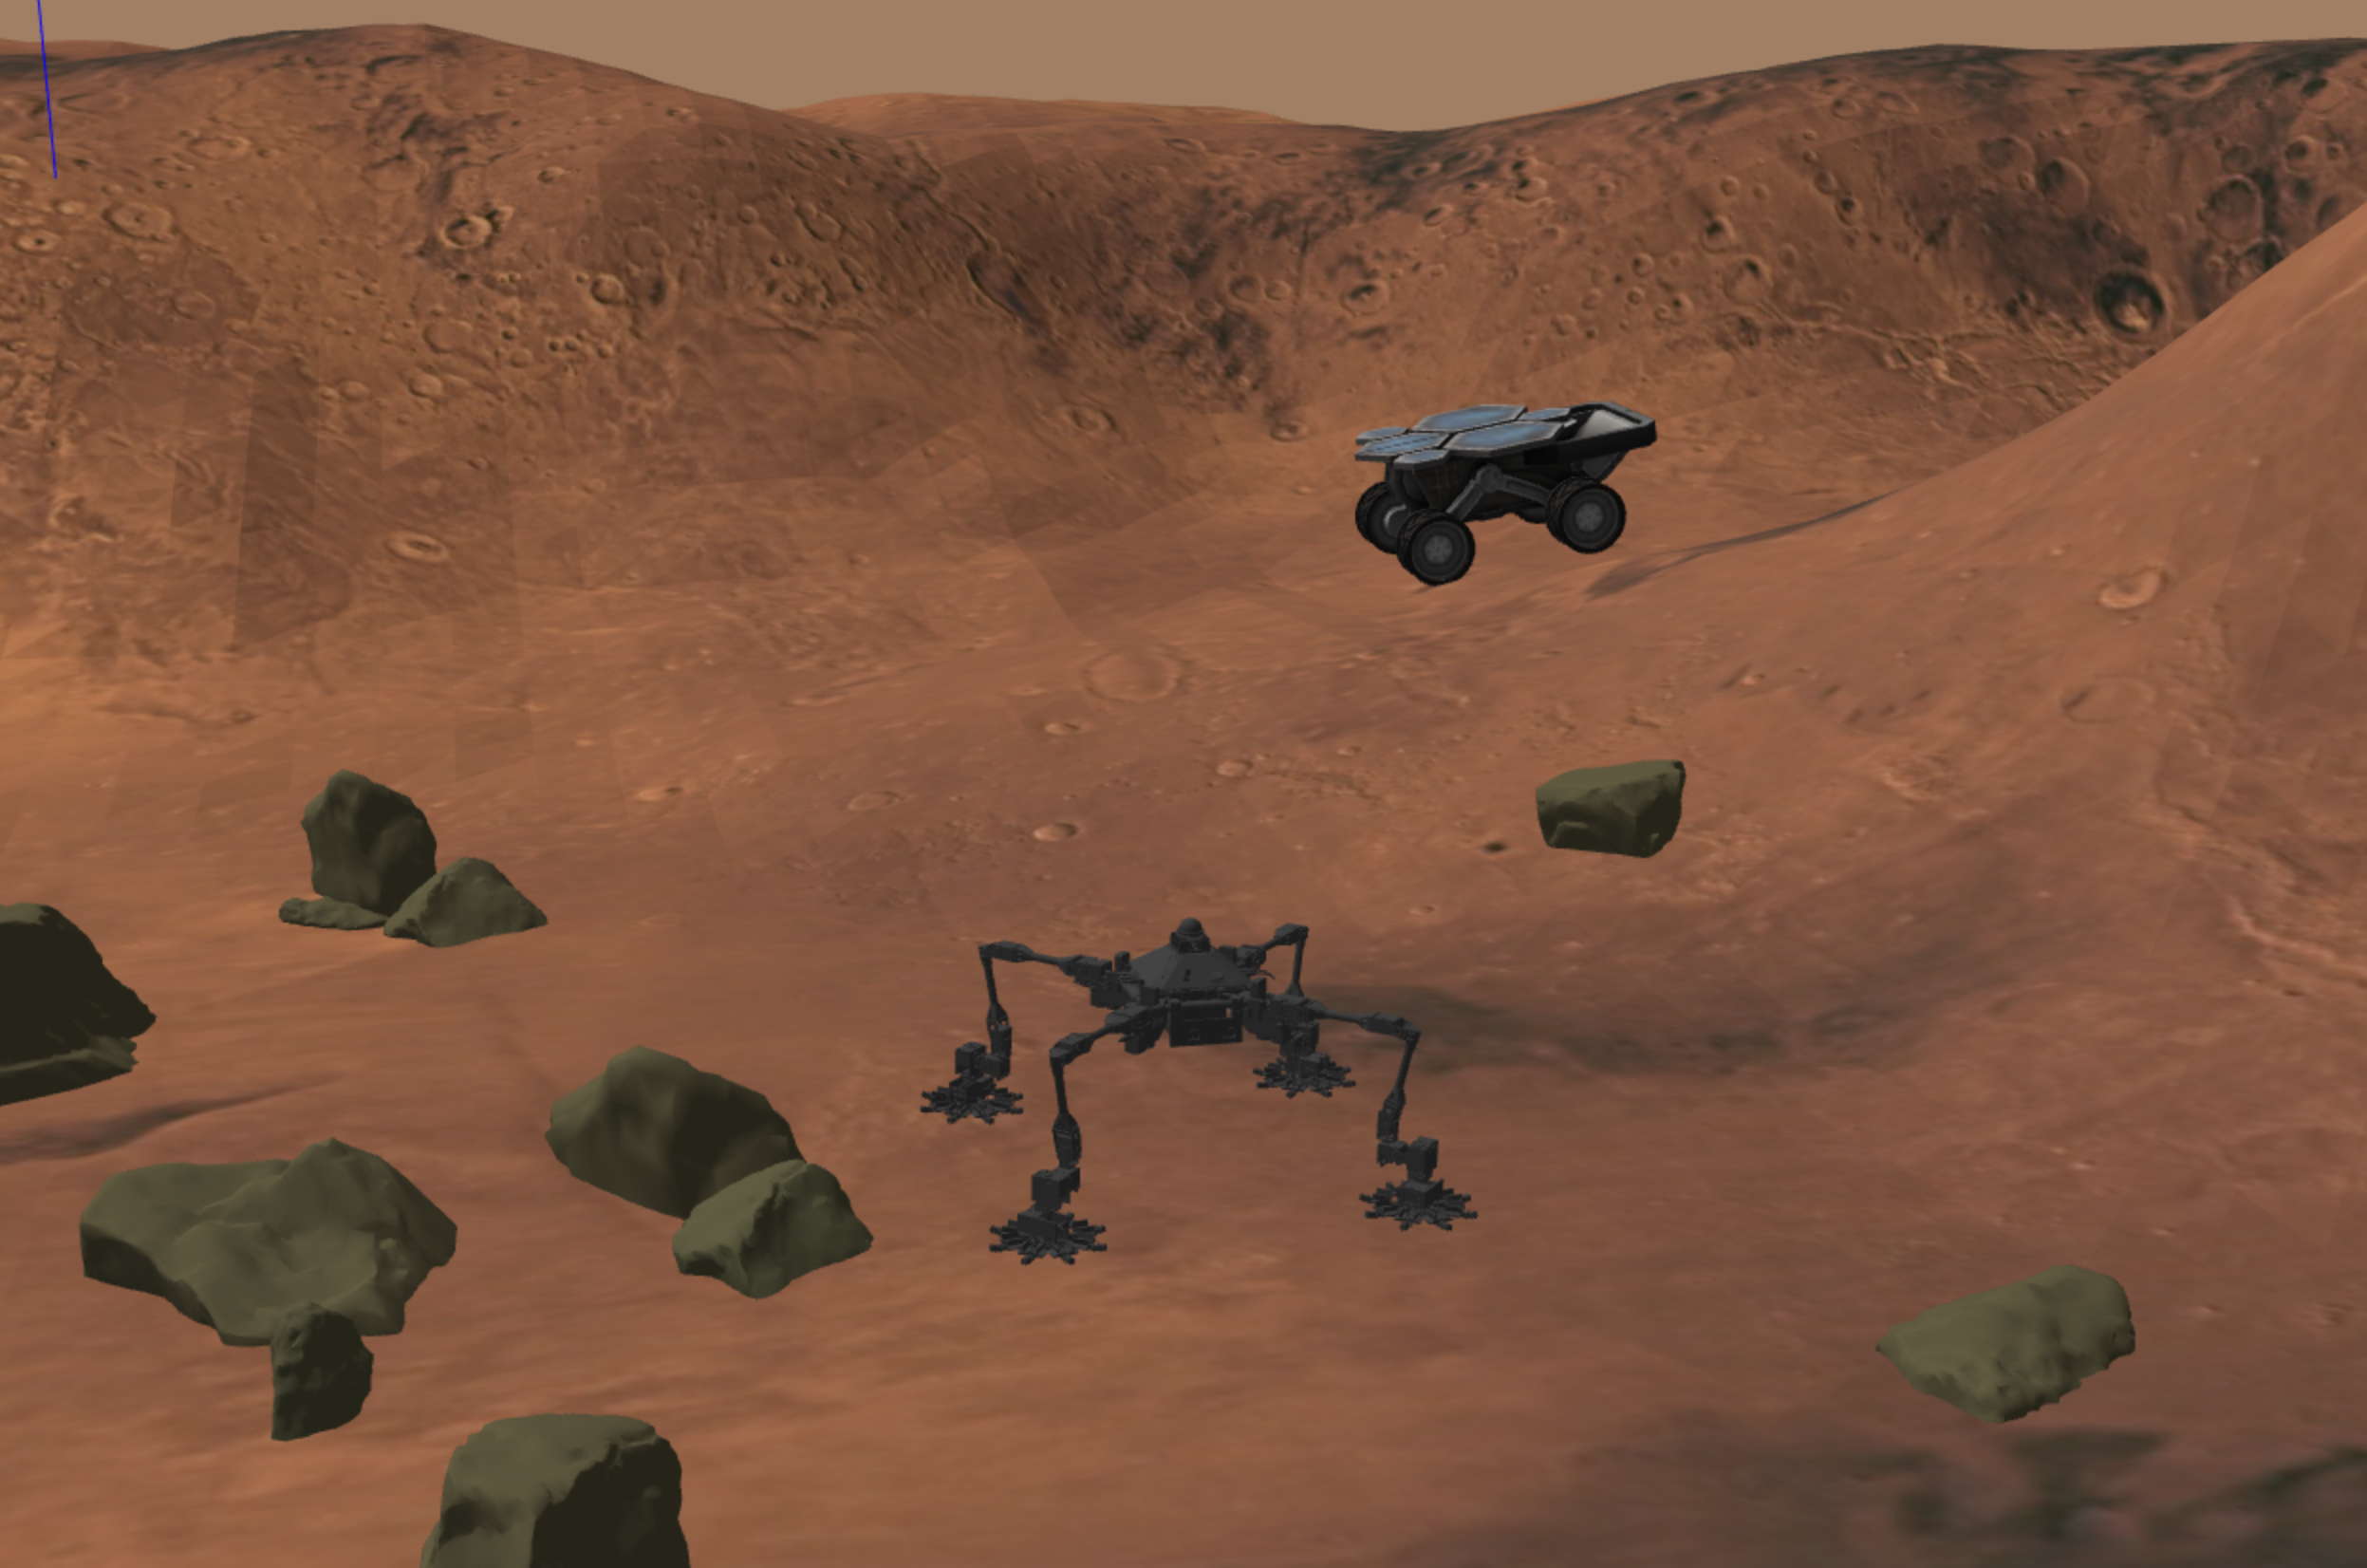
\includegraphics[width=0.8\textwidth]{Images/img_ch4/simulation_gz_classic_ex1.png}}
    
    \caption[Simulation in Gazebo Classic]{Simulation in Gazebo Classic}
    \label{fig:sim_classic}
\end{figure}

\begin{figure}[H]
    \centering
    \subfloat[Gripper mode\label{fig:sim_harmonic_a}]{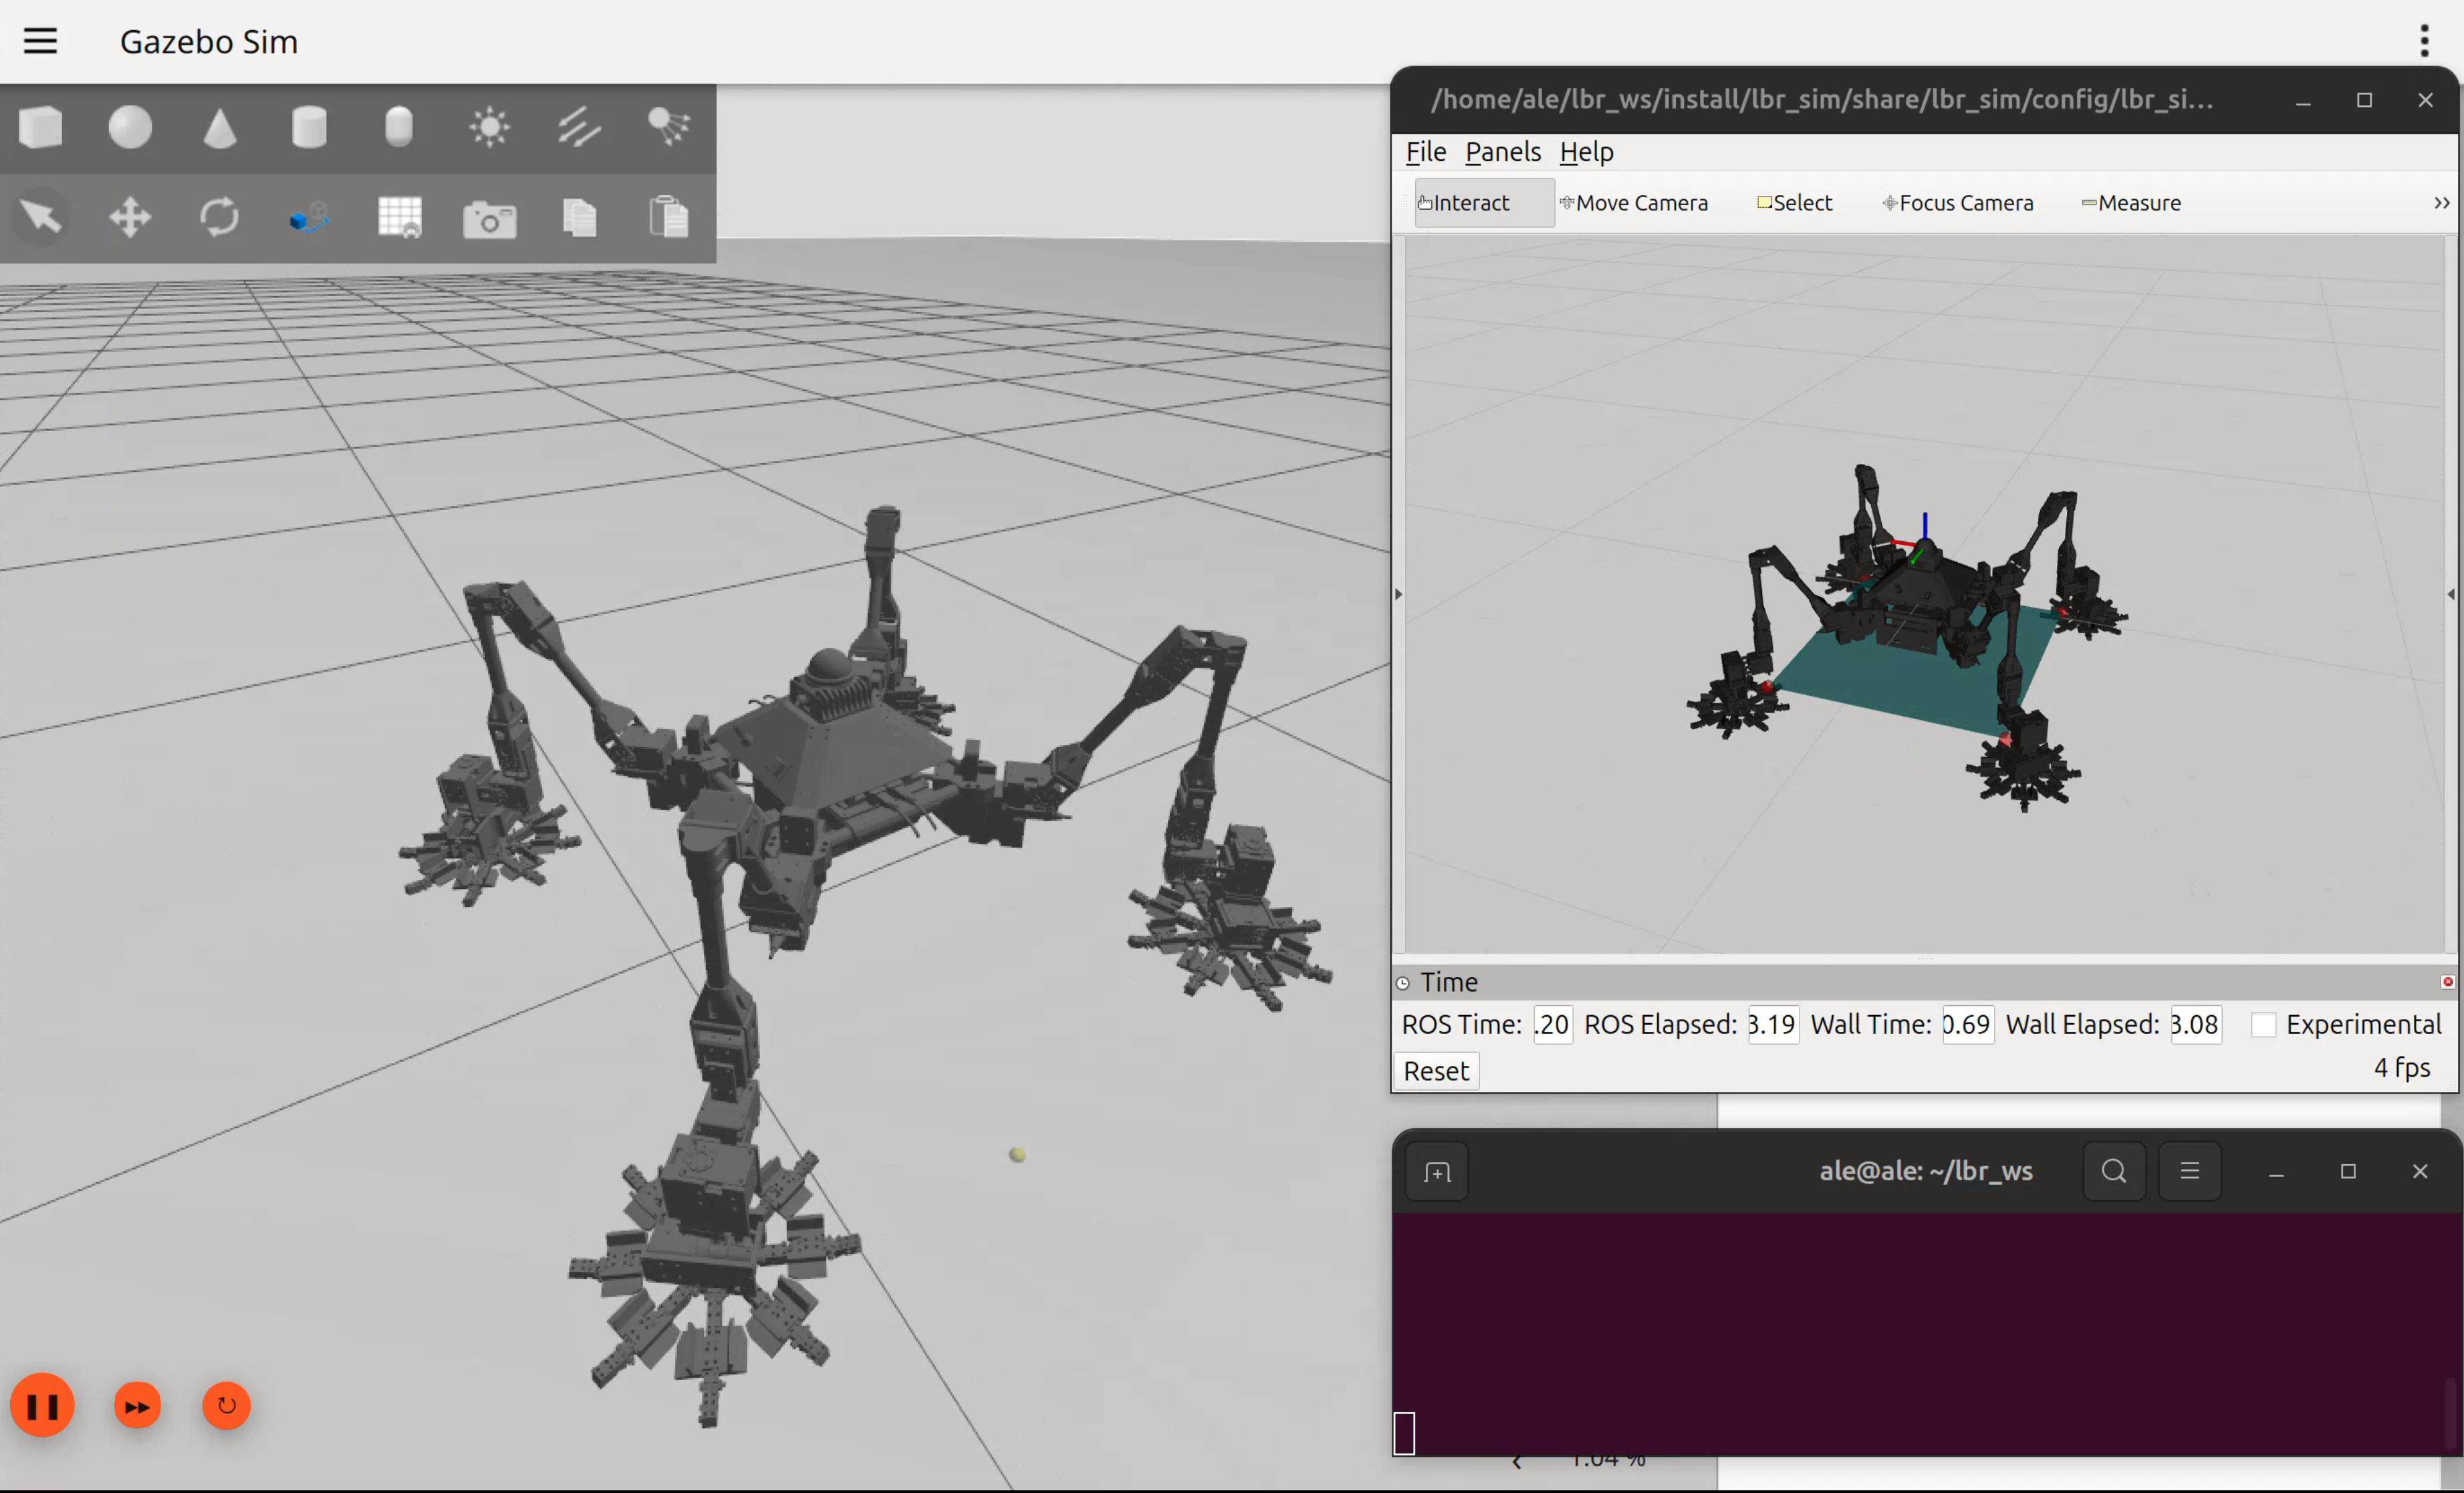
\includegraphics[width=0.40\textwidth]{Images/img_ch4/Harmonic_Gripper.png}}\quad
    \subfloat[Wheel mode\label{fig:sim_harmonic_b}]{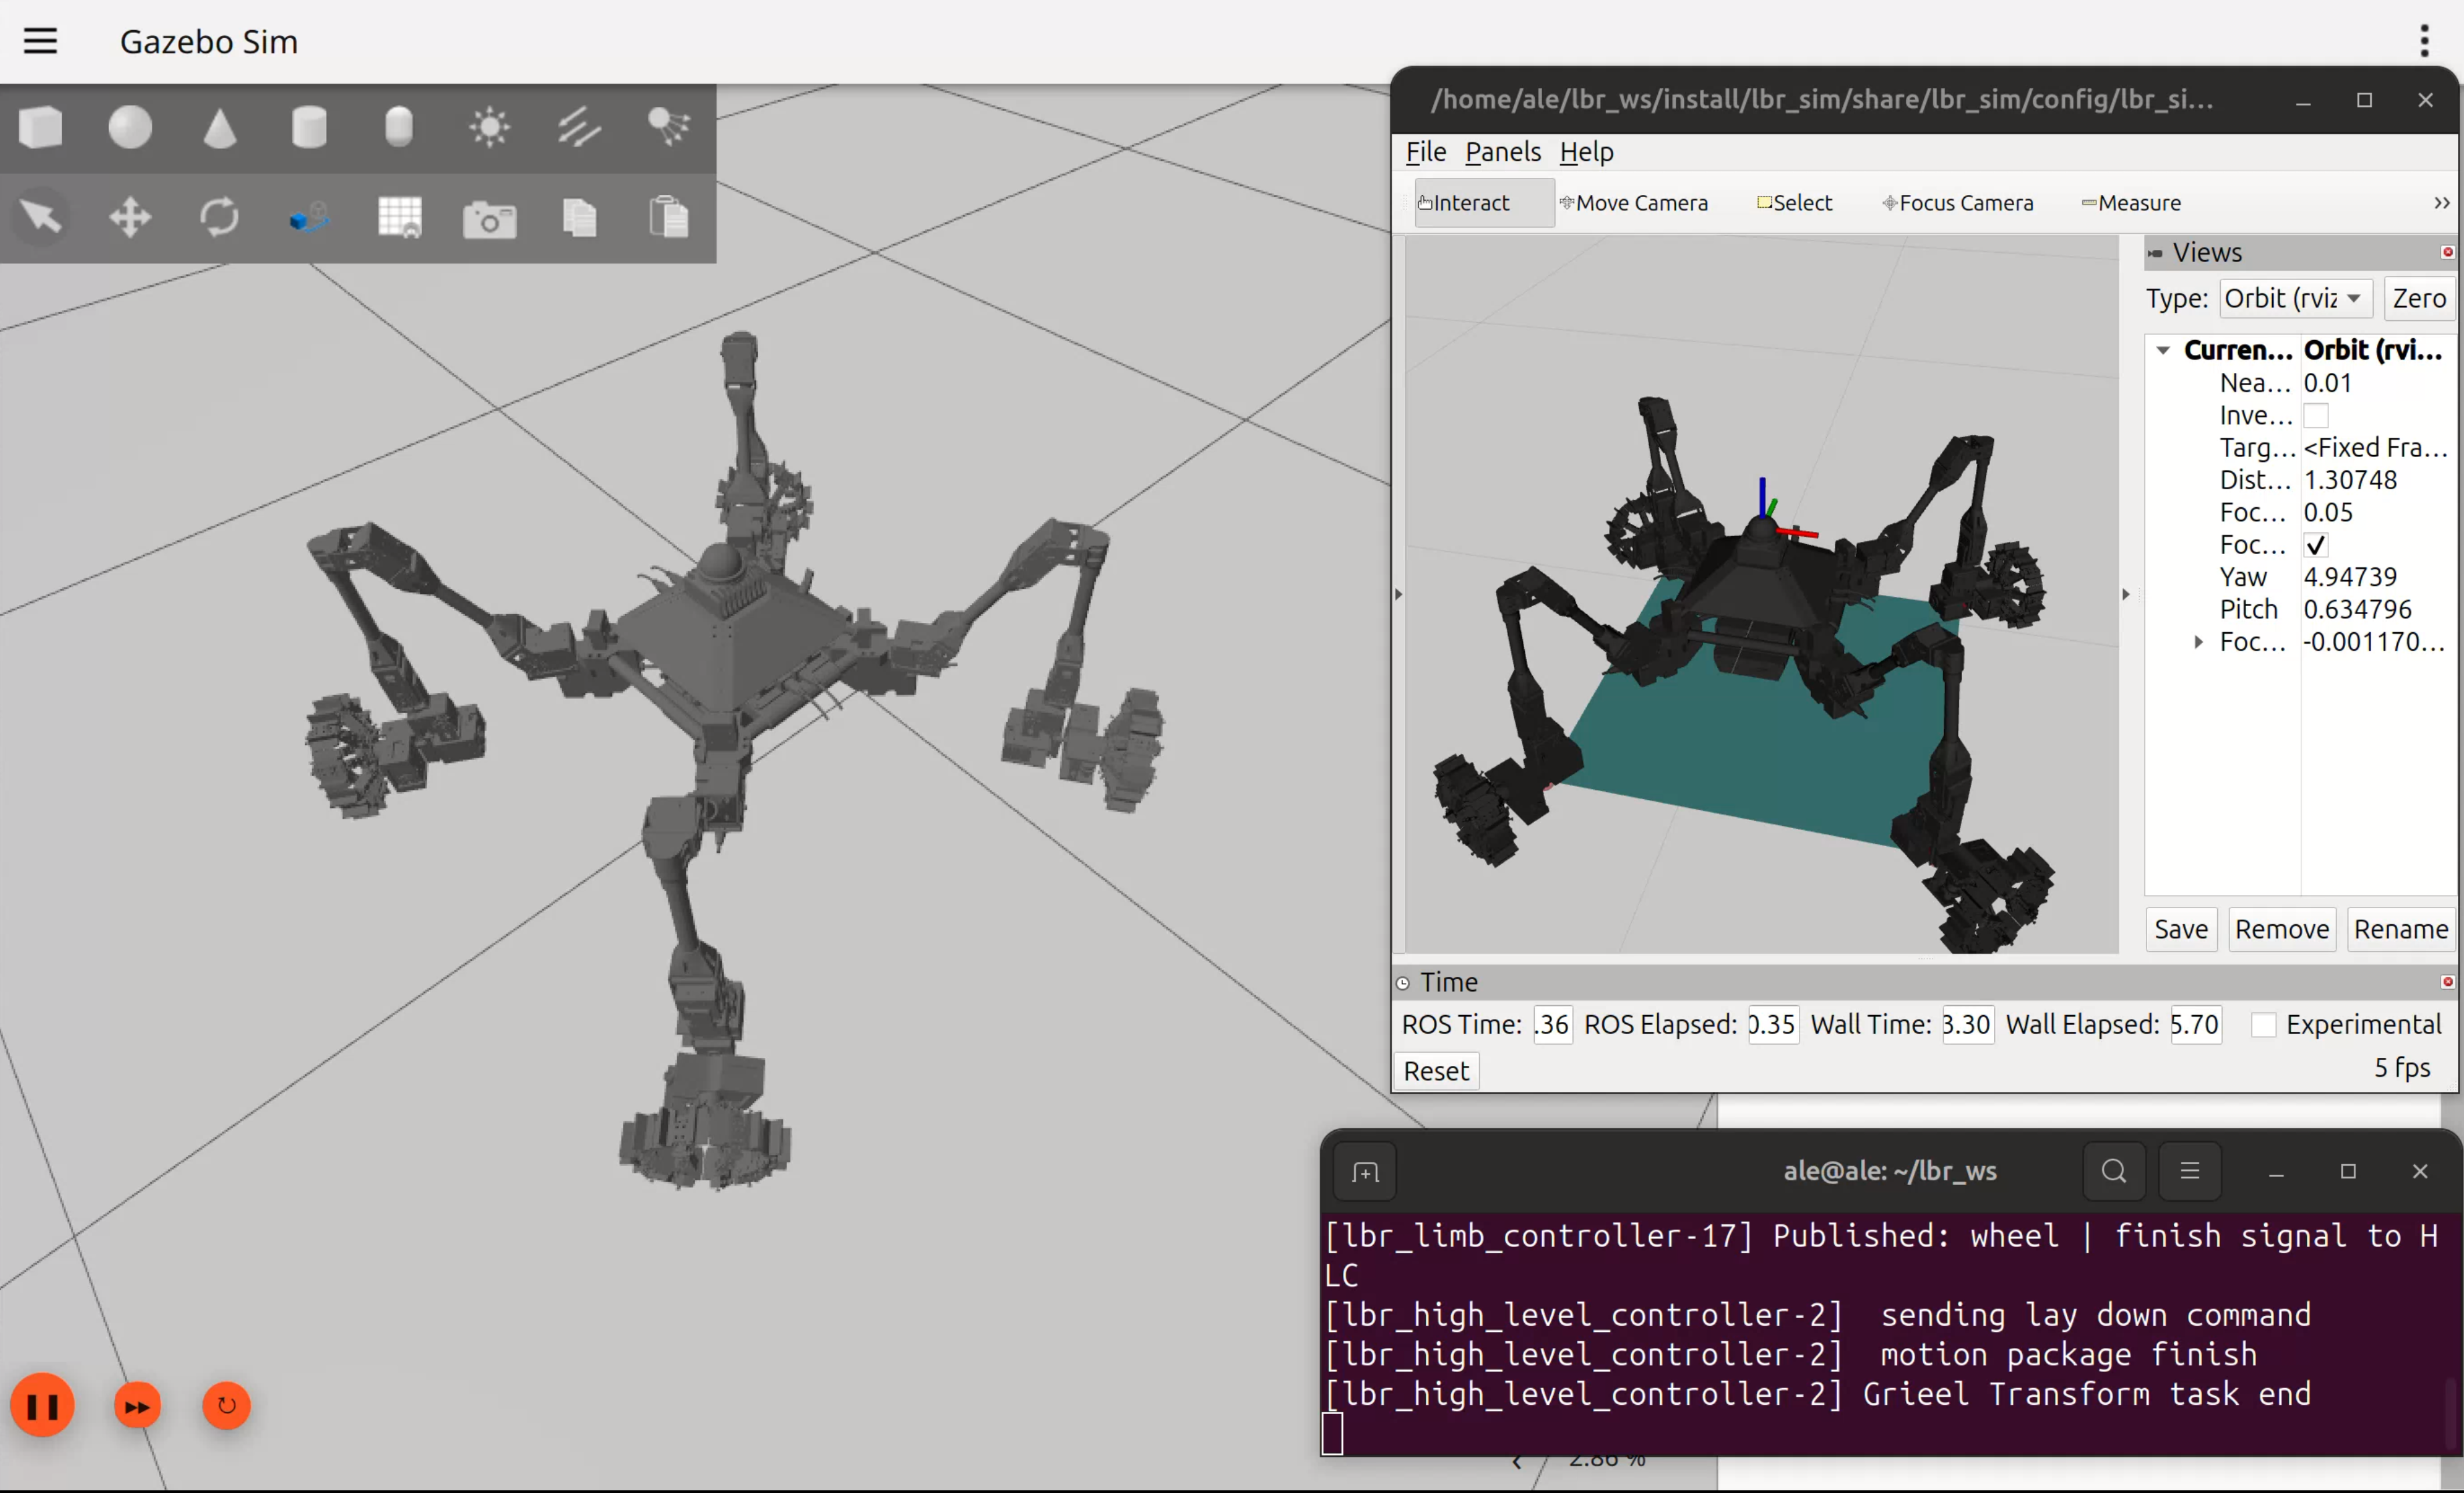
\includegraphics[width=0.40\textwidth]{Images/img_ch4/Harmonic_Wheel.png}}\\
    
    \subfloat[Mars environment\label{fig:sim_classic_c}]{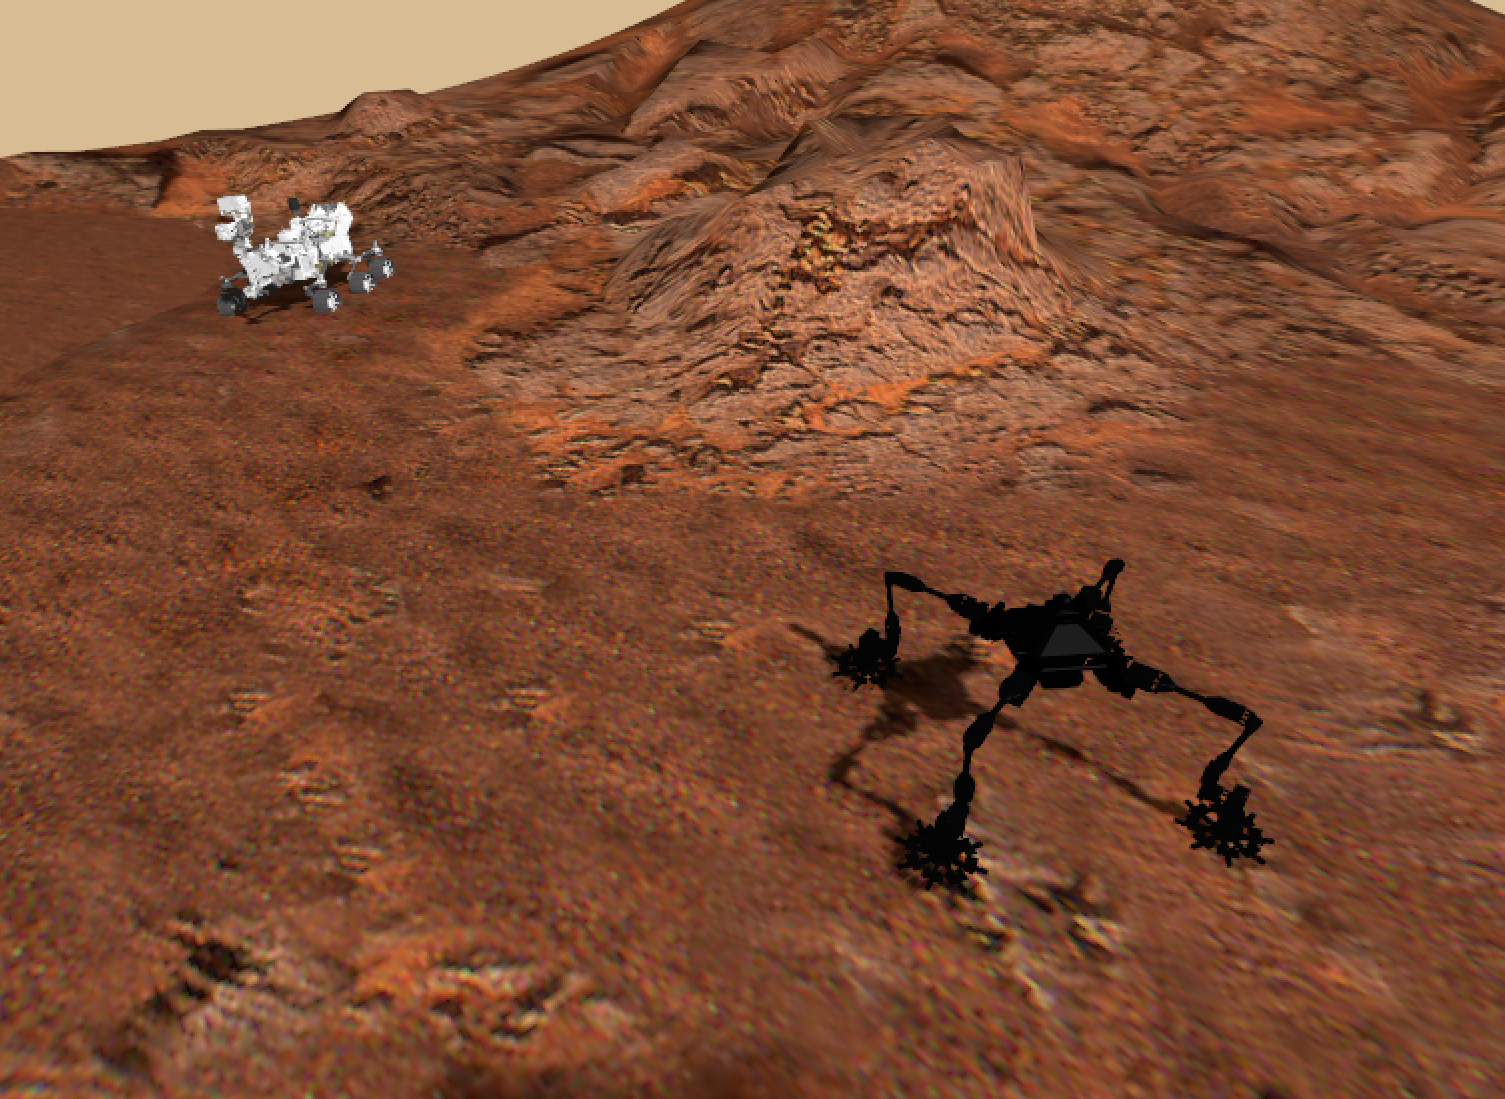
\includegraphics[width=0.8\textwidth]{Images/img_ch4/simulation_gz_sim_ex1.png}}
    
    \caption[Simulation in Gazebo Harmonic]{Simulation in Gazebo Harmonic}
    \label{fig:sim_harmonic}
\end{figure}

\subsection{MATLAB-Simulink Simulation}
\label{sec:matlab}

To improve the performance of joints' controllers, and test additional components on the controller, such as anti wind-up, filters, and feed-forward actions,  MATLAB provides the tools to perform analyses in the Laplace domain.
Simulink, a block diagram environment built on top of MATLAB, is a powerful tool for model-based control design and simulation. 

The first iterative tuning approach for the JTC, conducted in the Gazebo simulation environment (described in chapter \ref{sec:ros2_control}), was improved with a model-based approach in MATLAB-Simulink. Furthermore, the design of the IJC is based on the tests done in Simulink. 

To initialize the new simulator, the URDF model of the single LIMBERO-GRIEEL limb has been converted in DH format (reported in Fig\ref{fig:limbero_grieel_DH}), and represented as a robotic arm, with the convention used in the robotics toolbox by P.Corke\cite{CorkeMATLAB}.
% Some details on this convention transformation are described in Appendix\ref{ch:appendixA}, many tools to analyze serial links robotic structure exist, and this URDF to DH conversion has been an important aspect. 

After defining the limb model, it is possible to derive the dynamical matrices appearing in (\ref{eq:ManipulatorEoM}) and use it for model-based controller tuning.
Then, import the limb in Simulink and set up a block diagram for the motion control where testing its performance is simple. 

This approach considers only one limb and doesn't take into account the complex closed chain structure of LIMBERO-GRIEEL robot. 
Methods to implement a complex tree structure as a limbed robot and simulate it exist, with toolboxes such as the Robotic System Toolbox, based on Simscape Multibody.
Under the assumption of a high reduction ratio, the decoupled model described in section \ref{sec:DecoupledDyn} holds also for the multi-limbed structure. 
Nevertheless, because the limb behaves as a robotic arm that changes its fixed base:
\begin{itemize}
    \setlength\itemsep{-0.7em} 
    \item the limb root when not in contact
    \item the ground contact point if in contact
\end{itemize}
 a 2-state switching dynamic model has been considered for the limb. The dynamic properties change between the root-to-EE (raised) and the contact-to-root (in contact), and both models have been defined in MATLAB and tested. Further details on this aspect are given in the chapter \ref{sec:IJC} where the tuning approach is summarized.

The Simulink scheme used during control is reported in Fig.\ref{fig:Simulink} below, and the IJC is based on the scheme of Fig.\ref{fig:PPI_IJC}, with some additional components. 

\begin{figure}[H]
    \centering
    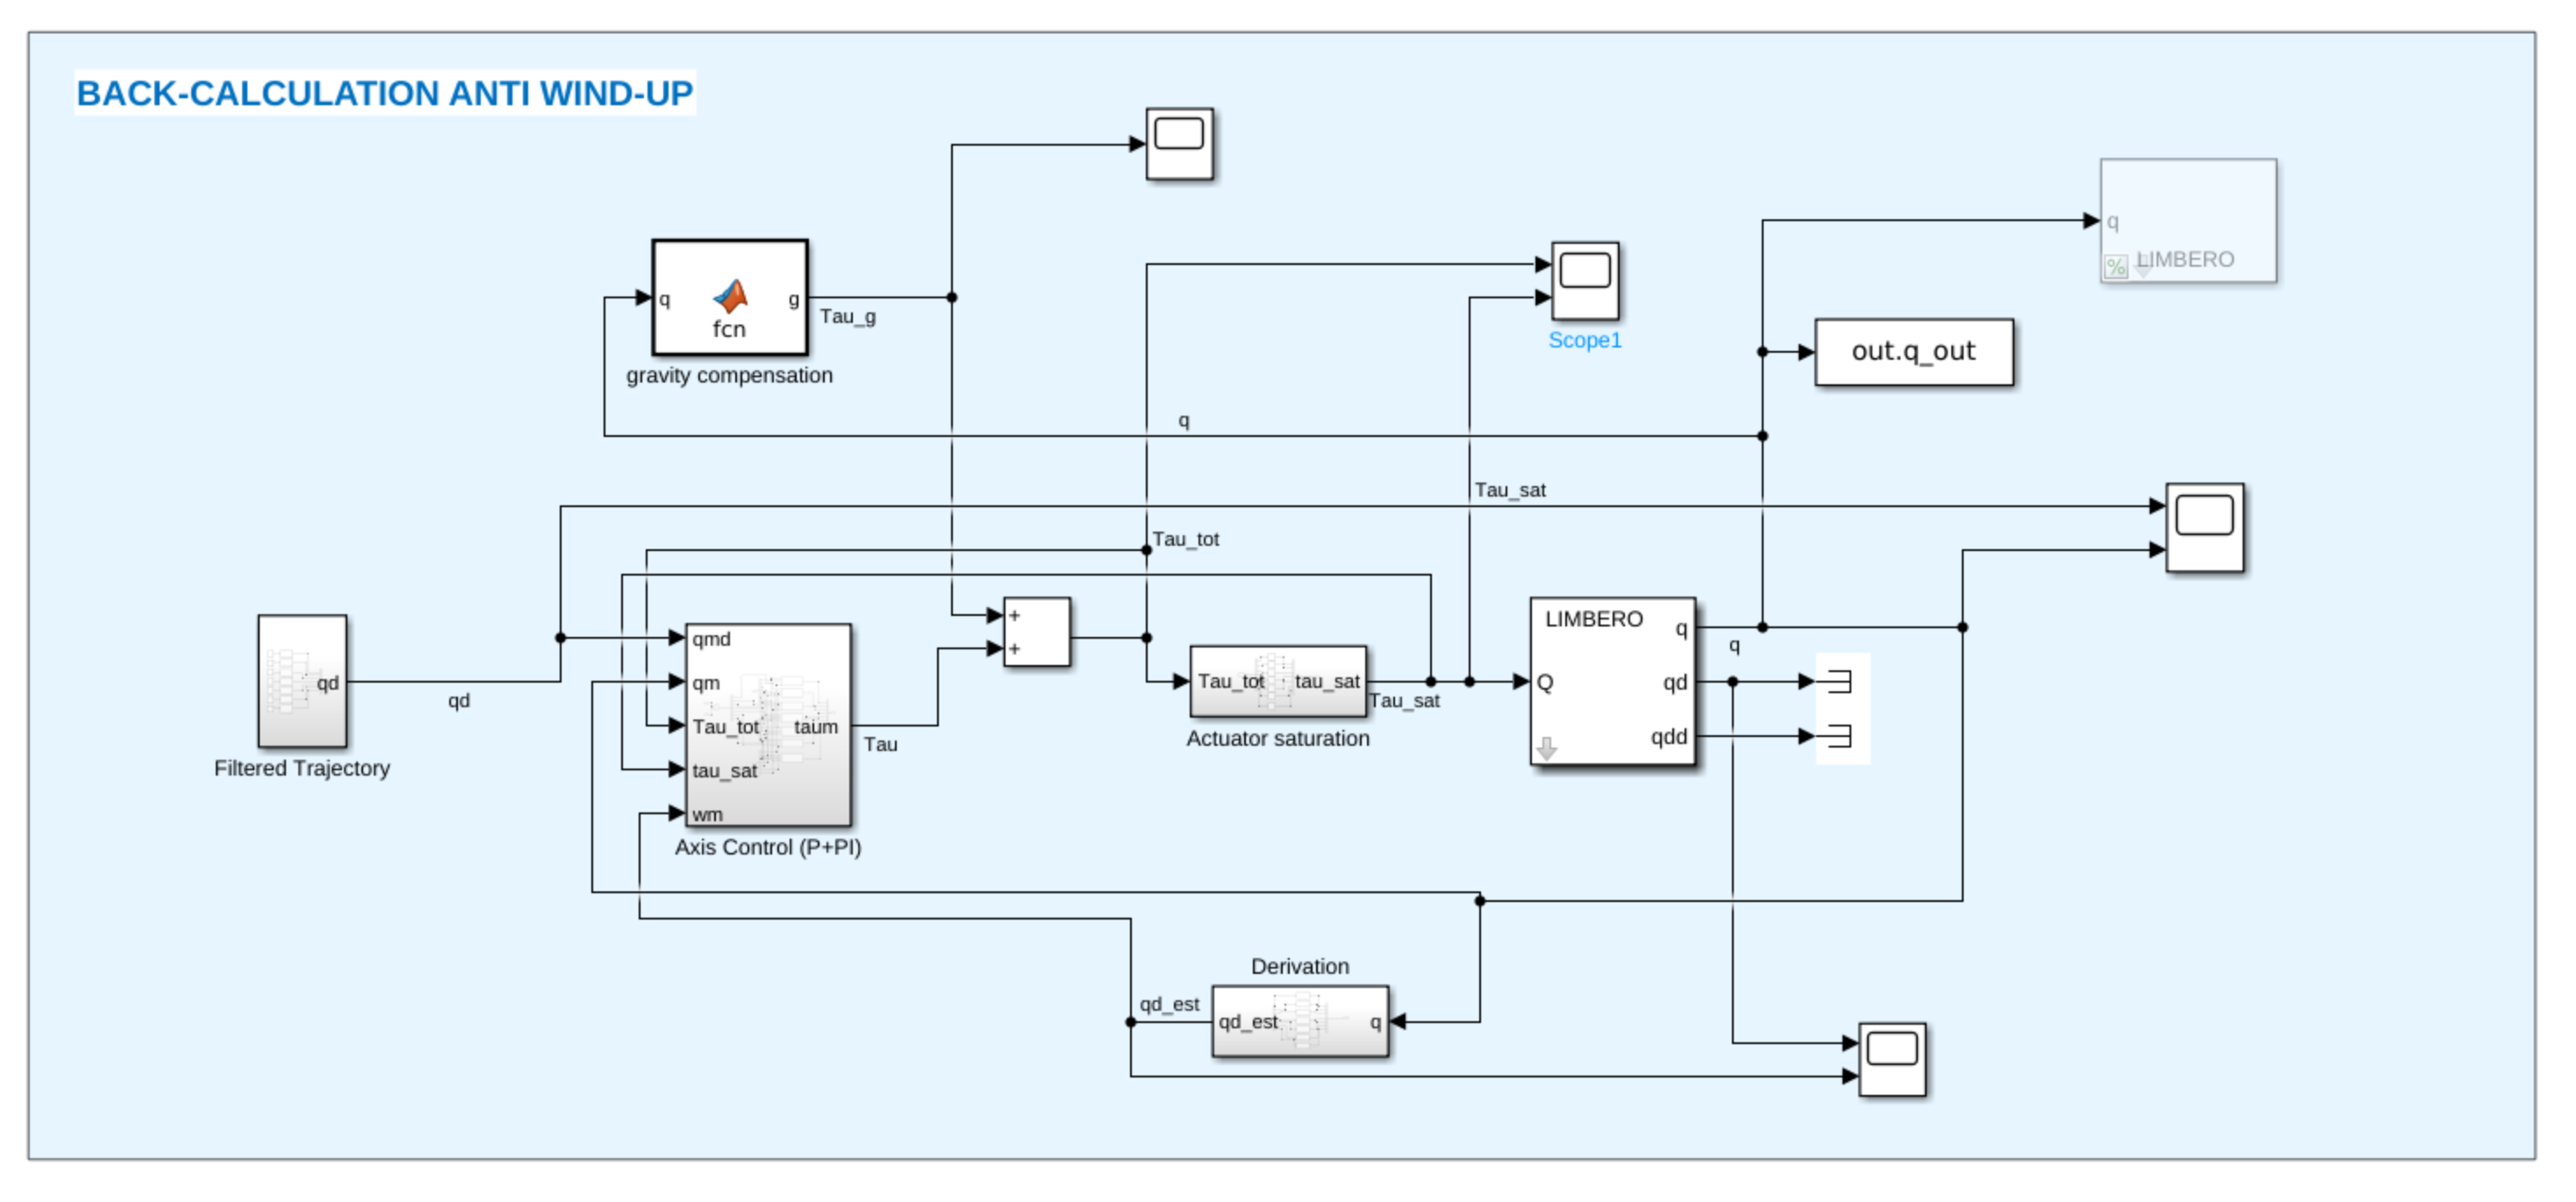
\includegraphics[width=1.1\textwidth]{Images/img_ch4/Simulink.png}
    \caption{Simulink scheme used to test single limb IJC performance}
    \label{fig:Simulink}
\end{figure}

Finally, MATLAB has been used to define a kinematic model of LIMBERO-GRIEEL and implement simple base task and limb tasks computation, used to test the BME theory derived in section \ref{sec:base_manipolability} and improve the transition algorithm described in the next section.


